\documentclass[a4paper,pra,aps,longbibliography,preprintnumbers,amsmath,amssymb,nofootinbib,floatfix,titlepage,openany,12pt]{book}

%  \usepackage[numbers, square]{natbib}
  \usepackage[style=numeric, backend=bibtex, sorting=none]{biblatex}
  \addbibresource{bib/refs.bib}
  \renewbibmacro{in:}{} % Remove the "In:" before the journal title

\defbibheading{myheading}[References]{%
    \chapter*{#1}%
    \addcontentsline{toc}{chapter}{#1}%
}


\ProvidesFile{biblatex.cfg}

% Customize the citation style
\DeclareNameAlias{sortname}{given-family}
\DeclareNameAlias{default}{given-family}
\renewcommand*{\labelnamepunct}{\addcomma\addspace}
\renewcommand*{\newunitpunct}{\addcomma\addspace}
\DeclareFieldFormat{title}{\mkbibquote{#1}}
\DeclareFieldFormat[article]{journaltitle}{#1}
\DeclareFieldFormat[article]{volume}{\textbf{#1}}
\DeclareFieldFormat[article]{pages}{}
\DeclareFieldFormat[article]{year}{#1}

% Custom format for DOI link with journal information
\renewbibmacro*{journal+issuetitle}{%
%  \usebibmacro{journal}%
%  \setunit*{\addspace}%
%  \printtext[bibhyperref]{%
%    \printfield{volume}%
%    \addcomma\space
%    \printfield{pages}%
%    \addspace
%    \printtext{(}%
%    \printfield{year}%
%    \printtext{)}%
%  }%
%  \setunit{\addcomma\addspace}%
%  \printfield{doi}%
%  \newunit
}
\DeclareFieldFormat[article]{doi}{%
  \ifhyperref
    {\href{https://doi.org/#1}{\thefield{journaltitle}\addspace\textbf{\thefield{volume}}, \thefield{pages} (\thefield{year})}}
}

% Use the "et al." abbreviation if more than two authors
%\DefineBibliographyStrings{english}{
%  andothers = {\textit{et al}\adddot}
%}


  \usepackage{graphicx}
%  \usepackage[italian]{babel}
%  \usepackage[numbers, sectionbib]{natlib}
  \usepackage{amsmath}
  \usepackage{listings}
  \usepackage{mathtools}
  \usepackage{amsfonts}
  \usepackage{amssymb}
  \usepackage{booktabs}
  \usepackage{braket}
  \usepackage{amsthm}
  \usepackage{siunitx}
  \usepackage{pdfpages}
  \usepackage{bm}
  \usepackage[suftesi]{frontespizio}
  \usepackage{xcolor}
  \usepackage{newfloat}
  \usepackage{wrapfig}
  \usepackage{tikz}
  \usetikzlibrary{patterns}
  \usepackage{comment}
  \usepackage{fancyhdr}
  \usepackage{geometry}
  \usepackage{chngcntr}
  \counterwithin*{footnote}{page}
  \usepackage{mathrsfs}
  \usepackage{epstopdf}
  \usepackage[breaklinks]{hyperref}
  %\usepackage[ocgcolorlinks, linkcolor={green!30!black},citecolor={red!40!black},urlcolor={blue}, breaklinks=true]{hyperref}
%   \renewcommand{\ref}[1]{\textcolor{red}{\fbox{\textcolor{green}{\ref{#1}}}}}
  \hypersetup{colorlinks, linkcolor={green!30!black},citecolor={red!40!black},urlcolor={blue}}

  \geometry{a4paper,top=2.0cm,bottom=3.0cm,left=3.8cm,right=2.0cm,%
heightrounded,bindingoffset=5mm}

  \pagestyle{fancy}
  \fancyhead{}
  \fancyfoot{}

  \newcommand{\pt}{\,\, .}
  \newcommand{\cm}{\,\, ,}
  \newcommand{\pc}{\,\, ;}
  \newcommand{\be}[1]{\begin{equation}
	  \label{#1}}
  %\newcommand{\lb}[1]{\label{#1}}
  \newcommand{\ee}{\end{equation}}

  \def\ba#1#2\ea{\begin{align}\label{#1}#2\end{align}}

  \renewcommand{\sectionmark}[1]{\markright{\thesection\ #1}}

  \renewcommand{\chaptermark}[1]{%
  \markboth{#1}{#1}}


  \fancyhead[LO]{ \rightmark}
  \fancyhead[RE]{ \leftmark}

  \fancyfoot[RO]{\thepage}
  \fancyfoot[LO]{\footnotesize{PhD PreThesis}}
  \fancyfoot[LE]{\thepage}
  \fancyfoot[RE]{\footnotesize{PhD PreThesis}}

  \renewcommand{\headrulewidth}{0.01pt}
  \renewcommand{\footrulewidth}{0.0pt}
  

  \theoremstyle{plain}
  \newtheorem{theorem}{Theorem}[section]

  \theoremstyle{plain}
  \newtheorem{corollario}{Corollario}[section]

  \theoremstyle{plain}
  \newtheorem{lemma}{Lemma}[section]

  \theoremstyle{definition}
  \newtheorem{definizione}{Definizione}[section]

  \theoremstyle{definition}
  \newtheorem{oss}{Osservazione}[section]

  \theoremstyle{plain}
  \newtheorem{prop}{Proposizione}[section]


  \newcommand{\numberset}{\mathbb}
  \newcommand{\C}{\numberset{C}}
  \newcommand{\R}{\numberset{R}}
  \newcommand{\N}{\numberset{N}}
  \newcommand{\Z}{\numberset{Z}}
  \newcommand{\D}{\numberset{D}}

  \renewcommand{\vec}{\bm}

  \DeclarePairedDelimiter{\norma}{\lVert}{\rVert}
  \DeclarePairedDelimiter{\abs}{\lvert}{\rvert}
  

  \DeclareFloatingEnvironment[
      fileext=lox,
      listname={Lista di Codici},
      name=Codice,
      placement=tbhp,
      within=section,
      chapterlistsgaps=off
  ]{codice}
  

  \definecolor{codegreen}{rgb}{0,0.6,0}
  \definecolor{codegray}{rgb}{0.5,0.5,0.5}
  \definecolor{codepurple}{rgb}{0.58,0,0.82}
  \definecolor{backcolour}{rgb}{1.,1.,1.}
 
  \lstdefinestyle{mystyle}{
    backgroundcolor=\color{backcolour},   
    commentstyle=\color{codegreen},
    keywordstyle=\color{magenta},
    numberstyle=\tiny\color{codegray},
    stringstyle=\color{codepurple},
    basicstyle=\footnotesize,
    breakatwhitespace=false,         
    breaklines=true,                 
    captionpos=b,                    
    keepspaces=true,                 
    numbers=left,                    
    numbersep=5pt,                  
    showspaces=false,                
    showstringspaces=false,
    showtabs=false,                  
    tabsize=2
   }
 
  \lstset{style=mystyle}

\begin{document}
   
\begin{frontespizio}

  \Logo{imm/logo.pdf}
  \Istituzione{Universit\`a di Pisa}
  \Divisione{Physics Department}
  \Scuola{PhD PreThesis}
  %\Titolo{Quantum phase transition behavior in\\unitary and dissipation time evolution}
  \Titolo{Out-of-equilibrium dynamics in \\round-trip and dissipation protocols}
  %\Sottotitolo{Analysis of out-of-equilibrium regimes: round trip and dissipation protocols}
  \Sottotitolo{Behavior of the quantum phase transitions}
  \NCandidato{Author}
  \Candidato{Francesco Tarantelli}
  \NRelatore{Supervisor}{Supervisor}
  \Relatore{Prof. Ettore Vicari}
  \Piede{Session 2023/2024}

\end{frontespizio}

%   \includepdf[pages=-,pagecommand={},width=\textwidth]{ .pdf}   

\frontmatter  
   
%   \include{cpt/ } 

\tableofcontents

   \chapter{Introduction}

The progress achieved in the control of nano-scales many-body systems has recently renewed the interest in understanding the out-of-equilibrium dynamic in quantum spin models~\cite{PSSV-2011-noneqcoll, GAN-2014-quantumsimulation}. Out-of-equilibrium, these efforts provided, for instance, a characterization of the unusual spreading of correlations and entanglement \cite{kormos2017real,lerose2020quasilocalized,tortora2020relaxation,lagnese2022quenches,scopa2022entanglement,castro2020entanglement,vovrosh2021confinement,rigobello2021entanglement}, as well as of the thermalization \cite{birnkammer2022prethermalization,james2019nonthermal,robinson2019signatures,chanda2020confinement}, in condensed-matter analogs of confined systems.


A deeper comprehension of the time evolution of the critical correlations and entanglement spreading is indeed sought by both the theoretical and experimental communities~\cite{ADM-2015-EntanglementReview}.

%%%%%%%%%%%%%%%%%%%%%%%%%%%%%%%%%%%%%%%%


In many-body systems, out-of-equilibrium dynamics show prominently as these systems approach critical points associated with phase transitions. Even when the timescale $\tau_s$ for varying system parameters is significantly extended, large-scale critical modes fail to reach equilibrium. This leads to a rich tapestry of dynamic phenomena at phase transitions, including hysteresis, coarsening, Kibble-Zurek (KZ) defect production
\cite{kibble1976topology,kibble1980some,zurek1985cosmological,zurek1996cosmological}, aging, and more. Such phenomena have been explored extensively in both theoretical and experimental settings, spanning classical and quantum phase transitions (see, for instance, Refs.                                                                                                                                                                             \cite{binder1987theory, cui2020experimentally, bray2002theory, weiler2008spontaneous,
dziarmaga2010dynamics, PSSV-2011-noneqcoll, ulm2013observation}  and related references).

Out-of-equilibrium scaling behaviors tend to emerge when slowly traversing a critical point, especially when doing so in the large-timescale $\tau_s$ limit. These scaling behaviors depend on several factors, including the nature of the transition (classical or quantum), its universality class, and the specific characteristics of critical dynamics in classical systems (as detailed in Refs. \cite{kibble1980some, zurek1996cosmological, dziarmaga2010dynamics, PSSV-2011-noneqcoll}.). Slow, or quasiadiabatic, passages through these critical points enable researchers to unveil universal features related to the emergence of long-range modes during thermal and quantum critical phenomena.

In both classical and quantum contexts, many-body systems are described by Hamiltonians that can be expressed as:

\ba{hlamt}
    H(t) \equiv H[w(t)] = H_c + w(t) H_p \,\,,
\ea

Here, $w(t)$ represents a time-dependent Hamiltonian parameter, while $H_c$ and $H_p$ are time-independent components. $H_c$ serves as the critical Hamiltonian at the transition point, which might denote a quantum continuous transition driven by quantum fluctuations or a classical continuous transition fueled by thermal fluctuations. $H_p$, on the other hand, embodies a nontrivial, relevant perturbation. Within quantum many-body models, it's generally assumed that $[H_c, H_p] \neq 0$. The tunable parameter $w$ controls the strength of the coupling with the perturbation $H_p$, and it's considered a relevant parameter guiding the continuous transition. Consequently, $w_c = 0$ marks the transition point. To explore the scaling properties of out-of-equilibrium dynamics during phase transitions, researchers employ time-dependent protocols where parameters like $w(t)$ are slowly varied, linearly in time, across the transition point at $w_c = 0$, employing a large timescale $t_s$.

The inevitable growth of out-of-equilibrium dynamics during phase transitions in the thermodynamic limit arises because large-scale modes cannot equilibrate the long-range critical correlations that emerge at the transition point. This holds true even when the parameter $w$ changes very slowly, and even in the limit of large timescales. Consequently, when starting from equilibrium states at the initial value $w_i$, the system cannot pass through equilibrium states corresponding to the values of $w(t)$ across the transition point. This departure from equilibrium results in distinctive out-of-equilibrium dynamic scaling phenomena, especially when observed in the limit of large timescale $\tau_s$. This scenario gives rise to the Kibble-Zurek (KZ) problem, which concerns the scaling behavior of the final number of defects after slow passages through continuous transitions from the disordered phase to the ordered phase.

Out-of-equilibrium scaling behaviors in many-body systems undergoing slow transitions across classical and quantum critical points exhibit intriguing similarities. These phenomena can be comprehensively analyzed within unified renormalization group (RG) frameworks, analogous to those employed to understand equilibrium scaling behaviors, which can be related through quantum-to-classical mappings. However, it's important to note that the out-of-equilibrium scaling behavior in classical systems depends on the chosen dynamics, whether it involves purely relaxation processes or conserved quantities, leading to different dynamic features.

The first part embarks on an investigation into the effects of slow round-trip variations in the Hamiltonian parameter $w(t)$, which entail multiple crossings of quantum and thermal transitions. These round-trip protocols are initiated from equilibrium conditions, traverse the transition point, and return to their initial state, with the timescale $\tau_s$ governing the slow-crossing regime in the large-$t_s$ limit.

The exploration encompasses both classical and quantum continuous transitions, characterized by emerging long-range correlations. Unified RG frameworks are utilized to derive general dynamic scaling behaviors applicable to both classical and quantum transitions, considering large timescale $\tau_s$ for round-trip KZ protocols and large system sizes $L$. This study builds upon existing dynamic RG frameworks used in standard one-way KZ protocols.

Notably, this study focuses on transitions between gapped phases characterized by short-range correlations, avoiding the complexities associated with gapless modes in ordered phases. This approach differs from standard KZ protocols, where systems transition from a disordered phase to ordered phases characterized by long-range correlations, leading to additional dynamic effects at large timescales, such as coarsening phenomena or the emergence of massless Goldstone excitations.


As the ensuing discussions reveal, while there are analogies in the scaling behaviors observed in standard one-way KZ protocols at classical and quantum transitions, these similarities only partially extend to round-trip KZ protocols. Significant differences emerge, especially when the extreme value $w_f > 0$ is held fixed and finite at the return point, a situation where classical systems exhibit well-defined scaling phenomena with hysteresis-like scenarios. In contrast, quantum systems encounter challenges in observing scaling behaviors along the return path due to rapidly oscillating relative phases between relevant quantum states, making the return trajectory highly sensitive to protocol parameters, such as $w_f$ and system size. This sensitivity is a consequence of the quantum unitary nature of dynamics, and it bears similarities to the behavior observed in quantum two-level models subject to round-trip protocols, akin to the Landau-Zener-Stückelberg problem.\\

%%%%%%%%%%%%%%%%%%%%%%%%%%%%%%%%%%%%%%%%%%%%%%



\begin{comment}

Out-of-equilibrium dynamic phenomena at
phase transitions, such as hysteresis and coarsening,
Kibble-Zurek (KZ) 
\cite{kibble1976topology,kibble1980some,zurek1985cosmological,zurek1996cosmological}
defect production, aging, etc., have
been addressed in a variety of contexts, both
experimentally and theoretically, at classical and quantum
phase transitions (see, e.g., Refs. 
\cite{binder1987theory, cui2020experimentally, bray2002theory, weiler2008spontaneous,
dziarmaga2010dynamics, PSSV-2011-noneqcoll, ulm2013observation} 
and references therein). Out-of-equilibrium scaling behaviors generally
emerge when slowly crossing a critical point, i.e. in
the large scale limit. They depend on the nature of the
classical or quantum transition, its universality class,
and the type of critical dynamics in classical systems, see e.g. Refs. 
\cite{kibble1980some, zurek1996cosmological, dziarmaga2010dynamics, PSSV-2011-noneqcoll}. 
Therefore, slow (quasi-adiabatic) passages through critical points allow us to
probe the universal features of the long-range modes
emerging at thermal and quantum critical phenomena \cite{tarantelli2022out}. 

In particular, the first part of this
work analyzes the application of a round-trip KZ protocol across a continuous quantum
phase transition. We take as paradigmatic model a Kitaev chain \cite{Kitaev-2001} in 
which the chemical potential changes linearity in time, following the function $t/t_s$ 
with the time $t$ and the time scale $t_s$.\\

\end{comment}



%%%%%%%%%%%%%%%%%%%%%%%%%%%%%%%%%%%%%%%%%%%%%%%%%%%%%%%%%

Since any experimental device is unintentionally coupled to the environment, a particular emphasis is put on the dynamics of \textit{open quantum systems}~\cite{BP-openquantumsystembook}.

When the interactions of a quantum system with its surroundings are sufficiently weak, the real-time evolution of such apparatuses emerges from the interplay between the unitary and dissipative dynamics of the whole setup~\cite{RV-2021-coherentanddissipativedynamicsreview}. These hypotheses are usually satisfied within \textit{Lindblad} frameworks, which underpin the modelization of most atomic, molecular, and optical devices (AMO)~\cite{BDS-2015-KeldyshOptical}. In such cases, the system is described in terms of a density matrix $\rho$, and the time evolution is controlled by \textit{Linblad Master equations}
\begin{equation}
    \frac{d\rho}{dt} = \mathcal{L}[\rho]\,.
    \label{eq_def_intro_lindblad}
\end{equation}
The system generally thermalizes to a Non-Equilibrium Steady-State (NESS) solution after a transitory time frame. However, determining whether the NESS is unique is a more subtle issue~\cite{N-2019-uniquenesslindblad, SW-2010-openuniquesolution}. A quantity of particular interest is the \textit{Liouvillian gap}, hereafter denoted as $\Delta_\lambda$. This energy scale sets the typical relaxation time required to make the NESS stand out, entailing a complete loss of information on the initial quantum state. Quantum memory devices, for example, would benefit from long relaxation times, therefore small $\Delta_\lambda$~\cite{CCP-2011-quantummemories}.

Several works have addressed the nature of the Liouvillian gap in one-dimensional open quantum systems, considering different lattice geometries and dissipation sources also in integrable models~\cite{Z-2015-relaxtimes}. Distinguished behaviors emerge when the dissipators are either isolated or in a relatively large number compared to the system size $L$.
On the one hand, with bulk dissipation acting on the whole network, the system is gapped in several paradigmatic spin chains, such as XX, XXZ, and Ising models~\cite{YWHWD-2021-artificialnetweork, Z-2015-relaxtimes, KS-2019-nonhermitiankitaevladder}. On the other hand, when the number of dissipative sources is constant, the Liouvillian gap generally vanishes with a distinctive power-law behavior in the thermodynamic limit, typically as $\sim L^{-3}$~\cite{KS-2020-boundarydephasing, TV-2021-dissipativeboundaries, Z-2011-XXXchaingap}. In particulare, we focus on homogeneous systems within hard walls and inhomogeneous systems where the particles are trapped
by space-dependent external potentials, such as harmonic traps. We model the dissipative particle-
decay mechanism by Lindblad master equations governing the time evolution of the density matrix.
The resulting quantum dynamics is analyzed in protocols starting from the ground state of the
Hamiltonian for $N_0$ particles, then evolving under the effect of one dissipative particle-loss defect,
for example at the center of the system. We study the interplay between time, size l and the number
$N_0$ of initial particles, considering two different situations: (i) fixed number $N_0$ of initial particles;
(ii) fixed ratio $N_0 /l$, corresponding to the thermodynamic limit of the initial equilibrium state.
The physical mechanisms tying together these two regimes are still unclear and are, also, one of the main focus in this thesis.% \cite{franchi2023Liouvillian}.

%\rev{INSERT HERE THE PART OF THE HOLE GEOMETRY}

Moreover, we investigate a $(1+1)$-dimensional Kitaev ring with local particle-decay dissipators arranged in a \textit{sunburst} geometry~\cite{FRV-staticsunburst, FRV-timesunburst, MS-2022-sunburstquench}.
Starting the protocol in the proximity of a Continuous Quantum Transition (CQT), we study the out-of-equilibrium dynamic using Renormalization Group (RG) arguments and Finite-Size Scaling (FSS) frameworks~\cite{C-1996-ScalingandRG, RV-2021-coherentanddissipativedynamicsreview}.

Finally, we address the out-of-equilibrium dynamics arising from quantum-quench (QQ) protocols 
(instantaneous changes of the Hamiltonian parameters) in many-body systems within their quantum
critical regime and in contact with (homogeneously coupled) thermal baths. We consider two classes
of QQ protocols. In one of them the thermal bath is used to prepare the initial finite-temperature
Gibbs state; then, after quenching, the thermal bath is removed and the dynamics of the system is
unitary. We also address a more complex QQ protocol where the thermal bath is not removed after
quenching, thus the quantum evolution is also driven by the interaction with the bath, which may
be described by appropriate master equations for the density matrix of the system, where a further
relevant time scale, or inverse decay rate, characterizes the system-bath coupling.


\subsubsection{Outline}
$ $

In the \textbf{Chapter} \ref{chp_out}, we introduce all the equations and the definitions
useful to present the original results in the last two chapters. Indeed, we give a brief
intro on the quantum phase transitions and, then, we explain two different mechanisms
which send the system out-of-equilibrium regime: the Kibble-Zurek mechanism and the
Lindblad mechanism.\\

In the \textbf{Chapter} \ref{chp_round}, we address the effect of a round-trip Kibble-Zurek
protocol near a continuous and a first order quantum phase transition, using the Finite Size Scaling 
framework. We will find results which diverge from the classic hysteresis cycle scenario.\\

In the \textbf{Chapter} \ref{chp_diss}, we analyze the effects of a local and a uniform
dissipation process on a second-order transition. We will focus on the interplay between
these two type of dissipation mechanism, trying to extract common properties and different
behaviors. Moreover, we focus also on the effects in the case in which we consider the
interaction of our quantum many-body system with a thermal bath characterized by an
uniform temperature $T$.

   
\mainmatter

  \renewcommand{\chaptermark}[1]{%
  \markboth{\chaptername
  \ \thechapter.\ #1}{}}

   \chapter{Out-of-equilibrium dynamics}

%\input{cpt/1secs_outeq/11intro}
\section{Introduction}

In the following work, we expose the analysis of the many-body systems in the presence of time-dependent perturbations. These interferences send 
\begin{align}
	\label{Hmany-body}
	H = H_c + w(t) H_p \,\,;
\end{align}

\be{evol_rho}
	\frac{d\rho}{dt} = - i\bigr[ H, \rho \bigr] + \mathbb{D}(\rho) \pt
\ee

\cite{TV-21}
\ref{evol_rho}




\section{Equilibrium Quantum Transitions}

\subsection{Continuous Quantum Transition (CQT)}
\label{CQTeq}

In the thermodynamic limit, i.e. infinite volume limit, same specific models could undergo a continuous phase transition. With the word phase, we intend the physical properties of the ground stare associated with the Hamiltonian and characterized by the values of the Hamiltonian parameters. If this phase changes driving one of this parameter, we are in the presence of a quantum transition and the point, in which that happens, is called transition point.

In the particular case of the CQT, the quantum ground-state properties are continuous close to the transition point, called also critical point. 
In this special point, the system develops a long-distance correlations and its microscopic behavior becomes negligible.

Independent from the local details, the global properties determine a notable universal critical behavior in which we collect different physical systems in universality class.
In terms of the Renormalization Group (RG) theory, the critical point and its universal behavior ase associated the fixed points of the RG flux. Hence, if we call $b$ the characteristic unit length of the system and if we define the RG transformation as the parameter rescaling respect $b$, the physical observables satisfy general scaling law unchanged along all the RG flux \cite{S99}.

From a physics point of view, we can interpret the factor $b$ like the spatial correlation length $\xi$ which diverges approching the critical point.
According to the renormalization group (RG)
theory of critical phenomena, these global properties may be the spatial dimension-
ality, the nature of the order parameter, the symmetry and the symmetry-breaking
pattern~\cite{PV2002}.

Moreover, at CQTs the systems develop an equilibrium and dynamic scaling be-
havior in the thermodynamic limit and their quantum functions satisfy scaling
power laws characterized by universal critical exponents~\cite{CV2014}.

\subsection{First Order Quantum Transition (FOQT)}
\label{FOQTeq}

Quasi-degenerate vacua naturally arise in the context of quantum phase transitions, after a spontaneous symmetry breaking. Their behavior and coexistence in the non-critical regime is governed by a first-order quantum transition.

It is characterized by the crossings of the lowest-energy states in the infinite-volume limit and in the absence of conservation laws \cite{plissetto2023scaling}.
Instead, in a finite system, the energy gap among these states remain different from zero, giving rise to the phenomenon of avoided level crossing.

FOQTs are associated with many important out-of-equilibrium effects s, including nucleations and metastability \cite{binder1987theory,bray2002theory}, coarsening \cite{chandran2012kibble}, and anomalous dependence on the boundary conditions \cite{pelissetto2020scaling,panagopoulos2018dynamic,campostrini2015quantum,pelissetto2018finite,rossini2018ground}.

\subsection{Models}
\label{Models}

\subsubsection{Quantum Ising}
\label{QIsing}

As a first toy model for the study of quantum phase transitions, we consider the quantum 1D Ising Model whose Hamiltonian is given by:

\be{HIsing}
	H(g, h) = - \sum_{x=1}^{L-1} \sigma^{(1)}_x \sigma^{(1)}_{x+1}
	- h \sum_{x=1}^L \sigma^{(1)}_x - g \sum_{x=1}^L \sigma^{(3)}_x \pc
\ee

where $L$ is the system size and $\sigma_x^{(k)}$ are the Pauli matrices on the 
$x^{\rm th}$ site.\\

This system develops a quantum critical behavior at $g = g_c = 1$
and $h=0$, belonging to the 2D Classical Ising universality class \cite{S99}. Instead, 
when $h$ is different from zero, the lowest states energy gap is not vanish.

Along the RG flux, the relevant parameters associated with the RG perturbations at the 
fixed point are $r = g-g_c$ and $h$. Their RG dimensions are respectively $y_r=1/\nu=1$
and $y_h = 15/8$, so that the length scale $\xi$ of the critical modes behaves as
$\xi \sim \abs{g-g_c}^{-1/y_r}$ for $h=0$, and $\xi \sim \abs{h}^{-1/y_h}$ for $g=g_c$.
The dynamic exponent $z$ associated with the vanish critical gap $\Delta \sim \xi^{-z}$
at the transition point, is given by $z=1$. The order parameter field, which distinguishes 
the two phases and is associated with the longitudinal operators $\sigma_x^{(1)}$, has a
RG dimension equal to $y_l = d+z-y_h=1/8$, while that associated with the transverse
operator $\sigma_x^{(3)}$ is equal to $y_t = d+z-y_r = 1$.\\

In the ferromagnetic phase $g<1$, the model undergoes a FOQT at $h=0$. Across this point,
the system remains non-critical and displays exponential decay of the correlation 
functions.

For $h=0$, the model presents a level-crossing of the two lowest-energy state in the
infinite volume limit, where the energy gap closes exponentially for $L\to \infty$, e.g.
for open boundary condition \cite{cabrera1987role}:
\be{isingfoqtgap}
	\Delta(g,L) = 2 g^L(1-g^2) \Bigr[ 1+ {\cal O}(g^{2L}) \Bigr] \pt
\ee
In the limit of small longitudinal magnetic field, i.e. $\abs{h \ll 1}$, the system
presents a Zeeman-like gap in energy between the 2 lowest states which introduces another
symmetry-breaking of the degeneracy. We can express an approximation of this gap using
standard perturbation theory in $h$ \cite{campostrini2014finite}:
\be{isingperthgap}
	{\cal E}(g,h\to 0,L) \simeq 2 h \sum_{j=1}^{L}
	\abs{\braket{\sigma_j^{(3)}}} \simeq 2hLM_0(g) \cm
\ee
with $M_0 = (1-g^2)^{1/8}$ the approximated longitudinal magnetization in the constrains
$h = 0$ and $L\to \infty$.



\subsubsection{Kitaev chain}
\label{kitaev}

Now, we introduce the following lattice model, called Kitaev model \cite{Kitaev_2001},
whose Hamiltonian describes the fermions interaction with the lattice and is given by:
\ba{Hkitaev}
    \hat{H}&=-\sum_{x=1}^{L-1} (\hat{c}^{\dagger}_{x}\hat{c}_{x+1} 
    + \hat{c}^\dagger_{x}\hat{c}^\dagger_{x+1}+{\rm h.c}.)
    - \mu\sum_{x=1}^{L} \hat{n}_x\,,
    %\label{Hkitaev}
\ea
where $\hat{n}_x\equiv\hat{c}^\dagger_x\hat{c}_x$ is the number operator on the site $x$, and the operators $\hat{c}_x, \hat{c}^\dagger_x$ satisfy the canonical anticommutation relations, thus $\{\hat{c}_x, \hat{c}_y\}=\{\hat{c}^\dagger_x, \hat{c}^\dagger_y\}=0$ and $\{\hat{c}_x, \hat{c}^\dagger_y\}=\delta_{xy}$. Applying the Jordan-Wigner transformation~\cite{S-1999-QuantumBook}, the Kitaev ring can be exactly mapped into a quantum Ising chain with a transverse field~\cite{P-1970-Isingmodel}. We point out that the transformation does not preserve also the same boundary conditions, so attention should be paid when recasting Eq.~\eqref{Hkitaev} in its bosonic counterpart~\cite{RV-2021-coherentanddissipativedynamicsreview}. Nonetheless, many bulk properties of the Ising model, such as the critical exponents at the CQT point, are preserved by the mapping; in fact, these phase transition belongs
to the same universality class of the 1D quantum Ising model.\\


The quantum Ising model with a transverse field is one of the most common theoretical laboratories where fundamental issues on quantum phase transition can be addressed, given our deep knowledge of the quantum correlations~\cite{S-1999-QuantumBook}. The model is characterized by a $\mathbb{Z}_2$ global symmetry under spin reflection along the longitudinal axis. In Eq.~\eqref{Hkitaev}, this symmetry is implemented by the transformation that maps $\hat{c}^{(\dagger)}_x\to -\hat{c}^{(\dagger)}_x$. At zero temperature, the ground state experiences a CQT at $\mu_c=-2$ and the $\mathbb{Z}_2$ symmetry is then spontaneously broken. The critical point separates a paramagnetic phase ($\abs{\mu}<\abs{\mu_c}$), where correlation functions are exponentially dumped, from an ordered phase ($\abs{\mu}<\abs{\mu_c}$), where correlation functions are instead long-range ordered. Close to the critical point, the correlation length diverges as $\xi\sim\abs{\mu-\mu_c}^{-\nu}$, where $\nu=1/y_g=1$ for Ising transitions. The gap $\Delta$, which describes the energy difference between the first excited state and the ground state, vanishes instead as $\Delta\sim\xi^{-z}$ with $z=1$. 





\section{Unitary time-evolution}



%\subsection{Quench}
\subsection{Dynamic Scaling Theory}

In the quench protocol, we define a family of Hamiltonians of type:
\ba{Hquench}
H(\bar \mu) = H_o + \bar\mu P \cm
\ea
where in this case the scaling variable $\bar \mu$ tunes the strength of the perturbation
$P$ such that $\Bigr[ H_o , P] \neq 0$ and $H_o$ is the unperturbed Hamiltonian 
whose parameters assume their critical values.

In this quench protocol, at $t = t_0$ the system starts in the ground state
of the Hamiltonian associated with an initial value $\bar \mu_i$ . Then, at time $t>0$, we
suddenly change the coupling from $\bar \mu$ to $\bar \mu _i$ and we follow the 
corresponding evolution of the system, described by the Schro\"odinger equation
in the form of the Von-Neumann equation:
\ba{eqschrodinger}
\partial_t \rho(t) = -i \Bigr[ \hat H(\bar \mu), \rho(t) \Bigr] \qquad \rho(t=0) = \rho_0 \,\,,
\ea
where $\rho(t)$ is the system density matrix at time $t\,$.

To express a possible scaling law, we define a further scaling variable associated
with the time:
\be{theta_din}
\theta = t \Delta \cm
\ee
which is obtained by recalling that the inverse energy difference of the lowest states
is proportional to the relevant time scale of the critical modes.

$ $\\

In the finite size system $\Delta _L \sim L^{-z}\,$, therefore in the infinite volume limit $L\to +\infty$, the out of equilibrium dynamics show a FSS behavior in which the scaling variable $\theta$ enters in the scaling functions. Hence, for this asymptotic dynamic scaling, we can write the following FSS law related to the correlation functions $F\,$: 
\begin{equation}  
\label{dfss-C}
F(\bm x, \bm y, \bar r, t;L) \approx u_l^{d+z-2+\eta} \,\mathscr{F}\Bigl(u_l\bm x ,u_l\bm y, \bar r\,u_l^{-1/\nu}, \bigl\{v_i\,u_l^{-y_i}\bigl\},  \bigl\{\widetilde{v}_i\,u_l^{-\widetilde{y}_i}\bigl\}, \theta  \Bigl) \,\,.
\end{equation}

\subsection{Kibble-Zurek mechanism}

The Kibble-Zurek(KZ) mechanism is related to the amount of final defects after slow
passages through continuous transition, from disordered to the ordered phase 
\cite{kibble1976topology, kibble1980some, zurek1985cosmological, zurek1996cosmological, 
zurek2005dynamics}. This type of out-of-equilibrium process is several studied both
analytically-numericallly \cite{dziarmaga2010dynamics, PSSV-2011-noneqcoll,
chandran2012kibble, rossini2021coherent} both experimentally \cite{weiler2008spontaneous,
ulm2013observation}.

The large-scale modes, associated with the changes of the transition tuning parameter, are
insufficient to equilibrate the long-distance critical correlations. Even in the large
time variation regime, the out-of-equilibrium dynamics grows in the thermodynamic limit.
In other words, when the system evolves, starting from an equilibrium state, the
time-evolution is different from an adiabatic dynamics and the system does not pass 
through equilibrium states.

In this scenario, the out-of-equilibrium regime is always describable in terms of the RG
framework and the equilibrium scaling behaviors can be related by the quantum to classical
mapping \cite{rossini2021coherent, S99}.




\section{Time-evolution in Open Quantum Systems}


\subsection{Lindblad framework}

To model the weak interaction between the previous quantum model and the surrounding
environment, we consider local external baths each in contact with only site of the system
chain. We work under the Born-Markov and secular approximations, so dissipators 
can be effectively modeled employing Lindblad quantum jump operators $\hat L_x\,$. 
In this limit, the time evolution of the density matrix can be described by Markovian
master equations in the Lindblad form as \cite{BP-openquantumsystembook, TV-21}:
\ba{eqlindblad}
	\frac{d\rho}{dt} = {\cal L}[\rho] = 
		-i \Bigr[ H, \rho \Bigr] + \mathbb{D}[\rho] \pc
\ea

where ${\cal L}$ is the Liouville superoperator, and $\mathbb{D}$ is the corresponding 
dissipation term, whose strength is regulated by the coupling $w$:
\ba{dissipator}
	\mathbb{D}[\rho] = & w \sum_{x \in {\cal I}} 
		\mathbb{D}_x[\rho] \cm \\
	\mathbb{D}_x[\rho] = &
		\hat L_x \rho \hat L_x^\dagger - 
		\frac{1}{2} \Bigl\{ \rho, \hat L^\dagger_x \hat L_x \Bigl\} \pc
\ea
where we indicate with ${\cal I}$ the set of the external baths in contact with the
quantum system.

\begin{comment}

\subsection{Thermal bath}

If we are interested to achieve an equilibrium Gibbs state at some temperature $T$, we
can consider the following modelization of interaction with a thermal bath within 
the Lindblad master equation \eqref{eqlindblad}.
Let us take a  quantum models described by quadratic Hamiltonians \cite{dr2021self}, 
such as that of the fermionic Kitaev model \eqref{Hkitaev}. This provides a relatively 
simple modelization of a thermal bath leading to thermalization in the large-
time limit of the corresponding Lindblad master equation
for the density matrix of the system.

The Kitaev Hamiltonian with open boundary conditions can be diagonalized 
in the Nambu field space by a Bogoliubov transformation \cite{dr2021self, PF70, bla86},
so that we can rewrite it as:
\ba{diagHKitaev}
	\hat H_K(\omega)  = \sum_{k=1} ^L \omega_k \hat b_k^\dagger \hat b_k  \cm
\ea
where $\omega_k$ are values of the spectrum of the Bogoliubov eigenoperators $\hat b_k$
(we are neglecting an irrelevant constant term). Note that both $\omega_k$ and 
$\hat b_k$ depend on the Hamiltonian parameter $\mu\,$. The relation between the
fermionic operators $\hat c_x$ and the Bogoliubov eigenoperators 
$\hat b_k$ can be generally written as \cite{dr2021self, PF70, bla86}:
\ba{basisfrombtoc}
	\hat c_x = \sum_{k=1}^L A_{xk} \hat b_k + B_{xk} \hat b^\dagger _k \cm
\ea
where $A$ and $B$ are appropriate $L{\rm x}L$ matrices depending on $\mu\,$.
Following Refs. \cite{dr2021self, CPR-2022-otto_engine}, we write the dissipator
$\mathbb{D}_T[\rho]$ in the Lindblad master equation \eqref{eqlindblad} in terms of
the Bogoliubov eigenoperators as:
\ba{thermaldissipator}
	\mathbb{D}_T[\rho] = & \gamma \sum_k \bigr[ 1 - f(\omega_k, T) \bigr] 
		\bigl( 2 \hat b_k \rho \hat b_k^\dagger -
			\{ \hat b_k^\dagger \hat b_k, \rho \} \bigl) + \\
		& + \gamma \sum _k f(\omega_k, T) \bigl( 2 \hat b_k^\dagger \rho \hat b_k -
                        \{ \hat b_k \hat b_k^\dagger, \rho \} \bigl) \cm
\ea
where:
\be{thermaldensityfunction}
	f(\omega_k , T ) = \bigl( 1 + e^{\omega_k/T} \bigl)^{-1} \pt
\ee
When using this dissipator term, the Lindblad master equation 
\eqref{eqlindblad} ensures the asymptotic large-time thermalization \cite{dr2021self}.
Therefore,
\ba{thermalstationarystate}
	\lim_{t \to \infty} \rho(t) & = \rho_t(\omega, T ) \cm \\
	\rho_t (w, T ) &  = \sum_n e^{-E_n(\omega)/T} \ket{\phi_n, \omega} 
					\bra{\phi_n, \omega} \cm
\ea
where $\rho_t(\omega,T)$ is the density matrix representing the
thermal state, $E_n (\omega)$ and $\ket{\phi_n, \omega}$ are the eigenvalues
and eigenstates of $\hat H(\omega)\,$. The asymptotic approach to
the thermal distribution is controlled by the decay-rate parameter $\gamma$.

\end{comment}

\subsection{Liouvillian gap}
\label{subsec_liouvilliangap}

Let us consider the following equation:
\ba{eigencalL}
	\widetilde{\cal L}[\widetilde \rho_i] = \lambda_i \widetilde \rho_i \cm
	\qquad \lambda_i \in \numberset{C} \pc
\ea
where $\widetilde {\cal L}$ is the (non-hermitian) Lindblad superoperator after the 
Choi-Jamiolkowski isomorphism 
\cite{BP-openquantumsystembook, VZ-2004-superoperatorvidal}, and $\widetilde \rho_i$ is the
density matrix eigen-operator associated with the complex eigenvalue $\lambda_i$.
In a few words, the transformation we have mentioned sends the density matrix $\rho$ to 
$\widetilde \rho$ through the mapping:
\be{vecrho}
	\rho_{ij} \ket i \bra j  \longrightarrow  \widetilde \rho_{ij} \ket i \ket j \pt
\ee
Therefore, the vectorized $\widetilde \rho$ lives in a $4^L$-dimensional Hilbert space.
In this basis, the action of $\widetilde{\cal L}$ on 
$\widetilde \rho$ can be written as follows:
\ba{vecteqlindblad}
	\widetilde{\mathcal{L}} =& -i \big(\hat{H} \otimes \hat{\mathbb{I}} 
		- \hat{\mathbb{I}}\otimes \hat{H}^t \big) + 
		w\sum_{x \in {\cal I}}\hat{L}_{x}\otimes \hat{L}^*_{x}\\
	&-\frac{w}{2}\sum_{x \in {\cal I}}\big(\hat{L}^{\dagger}_{x}\hat{L}_{x}
		\otimes\hat{\mathbb{I}}+\hat{\mathbb{I}}
			\otimes\hat{L}^t_{x}\hat{L}^*_{x}\big) \pt
\ea
It can be shown that all eigenvalues of $\widetilde{\cal L}$ satisfy 
$ {\rm Re}{\lambda_i } \le 0$ \cite{BP-openquantumsystembook}. The zero mode of the above 
operator represents the steady-state solution, namely, the NESS of the system. 
If $\hat L_x$ is not hermitian, the density matrix corresponding to the steady-state 
solution is not proportional to the identity matrix \cite{KS-2020-boundarydephasing}. 
We focus on the Liouvillian gap $\Delta_{\lambda}$, which is the non-vanishing eigenvalue
of ${\cal L}$ with the smallest real part:
\ba{Lioulliangap}
\Delta_{\lambda} = - \max_{i} {\rm Re}{\lambda_i } \pt
\ea
This quantity controls the typical relaxation time of the longest-living 
eigenmode differing from the NESS.


   \chapter{Round Trip variation of Hamiltonian parameter}

\section{The models}
\label{models}



\subsection{Quantum many-body systems}
\label{quamod}

As a paradigmatic quantum many-body system we consider the 1D quantum
Ising models, described by the Hamiltonian
\begin{eqnarray}
  H_{qI}(g,h) = - J \sum_{x=1}^{L} \sigma^{(1)}_{x\phantom{1}}
  \sigma^{(1)}_{x+1} - g \sum_{x=1}^L \sigma^{(3)}_x
  - h \sum_{x=1}^L \sigma^{(1)}_x\,,\quad
  \label{qisingmodel}
\end{eqnarray}
where $L$ is the system size, $\sigma^{(k)}_x$ are the Pauli matrices
on the $x^{\rm th}$ site ($k = 1,2,3$ labels the three spatial
directions). Periodic and antiperiodic boundary conditions
(respectively PBC and ABC) are set by requiring respectively
$\sigma^{(k)}_{L+1} = \sigma^{(k)}_1$ and $\sigma^{(k)}_{L+1} =
-\sigma^{(k)}_1$.

We recall that the quantum Ising model (\ref{qisingmodel}) develops a
quantum critical behavior at $g=g_c=J$ and $h=0$, belonging to the 2D
Ising universality class, see e.g. Ref.~\cite{S99}. The model
is always gapped for $h\neq 0$.  The relevant parameters $r\equiv
g-g_c$ and $h$ are respectively associated with even and odd RG
perturbations at the Ising fixed point.  Their RG dimensions are
respectively $y_r=1/\nu=1$ and $y_h=15/8$. The dynamic exponent $z$,
controlling the vanishing of the gap at the transition point, is given
by $z=1$. Moreover, we recall that the RG dimension of the
order-parameter field, associated with the longitudinal operators
$\sigma_x^{(1)}$, is given by $y_l=d + z - y_h=1/8$, while that
associated with the transverse operator $\sigma_x^{(3)}$ is given by
$y_t = d + z - y_r = 1$.  In the following we assume ferromagnetic
nearest-neighbour interactions with $J=1$, thus $g_c=J=1$.


To achieve round-trip protocols between gapped phases, without
degeneration of the lowest quantum states, we consider Ising chains
with PBC at $g=g_c$ driven by a time-dependent longitudinal field
$h(t)$, that is,  comparing with Eq.~(\ref{hlamt}), we identify
\begin{eqnarray}
  H_c = H_{qI}(g_c,0)\,,\quad w(t) = h(t)\,, \quad H_p = - \sum_{x}
  \sigma^{(1)}_x\,.
\label{isichoice}
\end{eqnarray}

The quantum Ising Hamiltonian $H_{qI}(g,0)$ for vanishing longitudinal
field $h$ can be mapped into a quadratic model of spinless fermions
through a Jordan-Wigner transformation~\cite{LSM-61, Katsura-62},
obtaining the so-called quantum Kitaev wire:~\cite{Kitaev-2001}
\begin{equation}
  H_{K}(\mu) = - \sum_{x} \big( c_x^\dagger c_{x+1} + c_x^\dagger
  c_{x+1}^\dagger + {\rm h.c.}  \big) - \mu \sum_{x} n_x \,,
  \label{kitaev2}
\end{equation}
where $c_x^{(\dagger)}$ is the fermionic annihilation (creation)
operator on site $x$ of the chain, $n_x\equiv c_x^\dagger c_x$ is the
corresponding number operator, and $\mu=-2g$.  Analogously to the
Ising spin representation, PBC and ABC are set by requiring
respectively $c_{L+1} = c_1$ and $c_{L+1} = -c_1$.  The Kitaev model
undergoes a continuous quantum transition at $\mu_c = -2g_c = -2$.  Of
course, it belongs to the 2D Ising universality class as well, so that
$y_\mu= y_r = 1/\nu=1$ (there is no an analogue of the longitudinal
field $h$ of the spin formulation (\ref{qisingmodel}) within the above
fermionic representation).  At the Ising transition the fermionic
operators $c_x$ and the particle density operator $n_x$ acquire the RG
dimensions $y_c=1/2$ and $y_n=1$, respectively.


Although the bulk behaviors of the Ising and Kitaev models in the
infinite-volume limit (and thus their phase diagram) are analogous,
some features of finite-size systems may significantly differ.  As a
matter of fact, the nonlocal Jordan-Wigner transformation of the Ising
chain with PBC or ABC does not simply map into the fermionic
model~\eqref{kitaev2} with PBC or ABC.  Indeed further considerations
apply~\cite{Katsura-62, PF70}, leading to a less straightforward
correspondence, which also depends on the parity of the
particle-number eigenvalue. In particular, we note that the Kitaev
quantum wire with ABC turns out to be gapped in both phases separated
by the quantum transition at $\mu_c=-2$. Indeed, it does not exhibit
the lowest-state degeneracy of the ordered phase of the quantum Ising
chain (namely, the exponential suppression of the gap with increasing
$L$).  The reason for such substantial difference resides in the fact
that the Hilbert space of the former is restricted with respect to
that of the latter, so that it is not possible to restore the
competition between the two vacua belonging to the
symmetric/antisymmetric sectors of the Ising model~\cite{Katsura-62,
  Kitaev-2001, CV2014, rossini2021coherent}.  Therefore, a continuous quantum
transition between gapped phases is also realized within the Kitaev
wire with ABC, by choosing
\begin{eqnarray}
  H_c = H_K(\mu_c)\,,\quad w(t) = \mu(t)-\mu_c\,,
  \quad H_p = - \sum_{x} n_x\,.\;\;
\label{kitchoice}
\end{eqnarray}


\subsection{Classical Ising model}
\label{classmod}

As a classical paradigmatic model undergoing a finite-temperature
continuous transition, we consider the 2D Ising model,
defined on a square lattice by the partition function
\begin{eqnarray}
  &&Z = \sum_{\{s_{\bm x}\}} e^{-\beta H_{cI}}\,,\qquad
  \beta=1/T\,, \label{partfunc}\\
  &&H_{cI}(J,h) = - J \sum_{\langle
    {\bm x} {\bm y} \rangle} s_{\bm x} s_{\bm y} - h
  \sum_{\bm x}
  s_{\bm x}\,,
\label{classisi}  
\end{eqnarray}
where ${\bm x}$ are the sites of the lattice, ${\langle {\bm x} {\bm
    y} \rangle}$ indicates the nearest-neighbour sites of the lattice,
$s_{\bm x}=\pm 1$ are classical spin variables, and $h$ is an external
homogenous magnetic field (we use the same symbol of the external
longitudinal field of the quantum ising model (\ref{qisingmodel}), but
this should not lead to confusion). We consider systems with PBC.  We
again set $J=1$.  The square-lattice Ising model (\ref{classisi})
undergoes a thermal continuous transition at $h=0$ and
$T_c=2/\ln(\sqrt{2}+1)$~\cite{Onsager-44}.  The critical behavior
belongs to the same universality class of the 1D quantum Ising
model. Therefore, it is characterized by the critical exponents
$\nu=1$ and $\eta=1/4$, and correspondingly the RG dimension
associated with the temperature relevant parameter is given by
$y_t=1/\nu=1$, and that associated with the odd external field $h$ is
$y_h = 2-\eta/2=15/8$, see e.g. Ref.~\cite{PV2002}.

Since we are going to discuss dynamic behaviors, we must also define
the type of dynamics driving the time evolution of the system.  We
consider a purely relaxational dynamics (also known as model A of
critical dynamics~\cite{HH-77,Ma-book}), which can be realized by stocastic
Langevin equations, or just Metropolis updatings in Monte Carlo
simulations~\cite{Metropolis:1953am}.  The corresponding dynamic
exponent $z$ has been accurately estimated by numerical studies,
obtaining $z\approx 2.167$ with an apparent relative precision that is
better than one per mille. Indeed, some of the most recent estimates
of the dynamic exponent $z$ for purely relaxational dynamics are
$z=2.1667(5)$ from \cite{NB-00}, $z=2.168(5)$ from \cite{WH-97},
$z=2.1665(12)$ from \cite{NB-96}, $z=2.172(6)$ from \cite{G-95},
$z=2.170(6)$ from Ref.~\cite{CV-11}, which have been obtained by
numerical analyses based on Monte Carlo simulations in equilibrium
conditions. In the following we use the estimate $z=2.167(1)$.

One may consider time-dependent KZ protocols also in this classical
context, supplementing the partition function (\ref{partfunc})
defining the classical Ising model with the purely relaxational
dynamics.  Analogously to the quantum case, cf. Eq.~(\ref{isichoice}),
we consider 2D Ising models with PBC at $T_c$ driven by a
time-dependent magnetic field $h(t)$. Therefore, we identify
\begin{eqnarray}
  & H_c = H_{cI}(1,0)\,,\qquad &\beta=\beta_c = {\ln(\sqrt{2}+1)\over
    2} \,, \label{clisichoice}\\ & w(t) = h(t)\,, \qquad &H_p
  = - \sum_{\bm x} s_{\bm x}\,.\nonumber
\end{eqnarray}



\section{One-way and round-trip KZ protocols across transition points}
\label{protocols}


In the following we assume the general Hamiltonian (\ref{hlamt}),
which represents the three models presented in Sec.~\ref{models} with
the identifications in Eqs.~(\ref{isichoice}), (\ref{kitchoice}), and
(\ref{clisichoice}).


\subsection{One-way KZ protocols}
\label{oneway}


KZ-like protocols have been largely employed to investigate the
dynamics of critical systems, at quantum transitions when the
many-body system is subject to unitary time evolutions, and at
classical thermal transitions considering, for example, a purely
relaxational dynamics which can be implemented by standard Langevin
equations~\cite{HH-77}.

\subsubsection{Quantum KZ protocols}
\label{quoneway}

In the case of quantum many-body systems, quasi-adiabatic passages
through the continuous quantum transition are obtained by slowly
varying $w$ across $w_c = 0$, following, e.g., the standard KZ
procedure:

(i) One starts from the ground state of the many-body system at
  $w_i < 0$, that is $|\Psi(t=0)\rangle \equiv |\Psi_0(w_i)\rangle$.
  
(ii) Then the out-of-equilibrium unitary dynamics, ruled by the
Schr\"odinger equation
  \begin{equation}
    {{\rm d} \, |\Psi(t)\rangle \over {\rm d} t} =
    - i \, \hat H[w(t)] \, |\Psi(t)\rangle \,,
    \label{unitdyn}
  \end{equation}
  arises from a linear time dependence of the Hamiltonian parameter
  $w(t)$, such as
  \begin{equation}
    w(t) = t/t_s \,,
    \label{wtkz}
  \end{equation}
  up to a final value $w_f>0$. Therefore the KZ protocol starts at
  time $t_i = t_s \, w_i<0$ and stops at $t_f= t_s \, w_f>0$.  The
  parameter $t_s$ denotes the time scale of the slow variations of the
  Hamiltonian parameter $w$.

Across a continuous transition, the growth of an out-of-equilibrium
dynamics is inevitable in the thermodynamic limit, even for very slow
changes of the parameter $w$, because large-scale modes are unable to
equilibrate as the system changes phase. Indeed, when starting from
the ground state associated with the initial value $w_i$, the system
cannot pass adiabatically through the ground states associated with
$w(t)$ across the transition point (in the infinite volume limit),
thus departing from an adiabatic dynamics.  Note that, in the quantum
cases that we consider, cf. Eqs.~(\ref{isichoice}) and
(\ref{kitchoice}), the slow variation of the longitudinal field $w$
brings the system from a gapped condition at $w_i<0$ to another gapped
condition for $w_f>0$. This somehow differs from the standard
situation of the KZ problem related to the defect production going
from disorder to order phases.~\cite{kibble1976topology, kibble1980some, zurek1985cosmological,
  zurek1996cosmological, zurek2005dynamics, polkovnikov2005universal, dziarmaga2005dynamics, PG-08, dziarmaga2010dynamics,
  Dutta-etal-book, chandran2012kibble}.







\subsubsection{Classical KZ protocols}
\label{cloneway}

In the case of many-body systems at classical thermal transitions, one
can again assume that slow passages through the continuous transition
are obtained by slowly varying $w$ across $w_c = 0$, following the 
classical KZ procedure:

(i) One starts from an equilibrium thermalized configuration at $w_i <
0$.
  
(ii) Then the out-equilibrium classical dynamics, ruled by the
relaxational Langevin equation~\cite{HH-77}, or a standard Metropolis
upgrading~\cite{Metropolis:1953am} of lattice configurations, arises
from linear changing of the parameter $w(t)$, as $w(t) = t/t_s$, up to
a final value $w_f>0$.  In the case of Metropolis-like dynamics, this
can be achieved by incrementing the time by one unity after one global
sweep of the lattice variables (Metropolis upgrading of all lattice
spin variables).  Again the KZ protocol starts at time $t_i = t_s \,
w_i<0$ and stops at $t_f= t_s \, w_f>0$.

Since the above protocol involves a stocastic relaxational
process, results are obtained by averaging over an ensemble of
trajectories (starting from an ensenble of thermalized configurations
at $w_i$), obtained following the above protocol.

We remark again that the classical out-of-equilibrium phenomena
associated with the above protocol occurs between two phases, for
$w<0$ and $w>0$, with short-ranged correlations.  This is again
different from standard classical protocols associated with the KZ
problem, in which one passes from a disordered to an ordered phase
characterized by long-range correlations, where further important dynamic
effects may set in, such as coarsening phenomena~\cite{chandran2012kibble},
in particular when the global symmetry is preserved by the KZ protocol
and its initial state, such as coarsening phenomena or massless
Goldstone excitations.



\subsection{Round-trip KZ protocols}
\label{rtpro}


We now consider round-trip protocols in which the Hamiltonian
parameter $w(t)$ varies linearly from $w_i<0$ to $w_f>0$, which is
analogous to the one-way KZ protocol, and then linearly decreasing it
back to the original value, crossing twice the transition point. For
quantum systems:

(i) One starts at $t=t_i$ from the ground state of the many-body
system at $w_i < 0$, given by $|\Psi(t_i)\rangle \equiv
|\Psi_0(w_i)\rangle$.
  
(ii) The out-equilibrium unitary dynamics, ruled by the Schr\"odinger
equation (\ref{unitdyn}), is driven by linearly increasing $w(t)$: as
$w(t) = t/t_s$ from $w_i<0$ (at time $t_i=w_i t_s<0$) to $w_f>0$ (at
time $t_f = w_f t_s>0$).

(iii) Then, for $t>t_f$ the dynamics is ruled by the Schr\"odinger
equation (\ref{unitdyn}) with an external field $w(t)$ that decreases
linearly with the same time scale $t_s$, from $w_f>0$ to the original
value $w_i<0$, closing the cycle.

To simplify the protocol, reducing its number of parameters, we
consider a {\em symmetric} round-trip protocol (an extension of the
later results to the most general case is straightforward) in which we
fix
\begin{equation}
  w_\star = w_f = - w_i \,,
  \label{wstardef}
  \end{equation}
and write the time dependence of $w(t)$ as
  \begin{eqnarray}
  w(t) = {{\cal T}(t)\over t_s}\quad {\rm for}\;\; t_i=-t_\star \le t
  \le 3t_\star\,,
\label{wtrtripdef}
\end{eqnarray}
where
\begin{equation}
  {\cal T}(t) = t_\star - |t-t_\star|
\label{triafunc}
\end{equation}
is the {\em triangular} function going linearly from ${\cal
  T}(-t_\star)=-t_\star$ to ${\cal T}(t_\star)=t_\star$, and then back
to ${\cal T}(3t_\star)=-t_\star$. The parameter $t_s$ represents the
time scale of the variation. The parameter $t_\star>0$ controls the
extension, i.e.  the starting and final times, of the protocols, from
$t_i=-t_\star$ to $t_f = 3 t_\star$, and also the interval of
variation of $w(t)$, from $w(t_i)=-t_\star/t_s$ to $w(t_\star) =
t_\star/t_s$.

Analogously to the quantum case, we extend the one-way KZ protocol for
classical systems to round-trip protocols, by taking the
time-dependent parameter $w(t)$ as in Eq.~(\ref{wtrtripdef}), with the
same definitions.



\section{Observables to monitor the out-of-equilibrium dynamics}
\label{obsdyn}

\subsection{Quantum case}
\label{quobs}

The resulting out-of-equilibrium evolution of quantum many-body
systems can be investigated by monitoring observables and correlations
at fixed time.  To characterize the departure from adiabaticity along
the slow dynamic across the continuous transition, we monitor the
adiabaticity function
\begin{eqnarray}
  A(t) = |\langle \, \Psi_0[w(t)] \, | \, \Psi(t) \, \rangle|\,,
  \label{adtfunc}
\end{eqnarray}
where $|\,\Psi_0[w(t)]\,\rangle$ is the ground state of the
Hamiltonian $H[w(t)]$, i.e. at instantaneous values of $w(t)$,
while $|\,\Psi(t)\,\rangle$ is the actual time-dependent state
evolving according to the Schr\"odinger equation (\ref{unitdyn}).

The adiabaticity function measures the overlap of the time-dependent
state with the corresponding ground state of the Hamiltonian at the
same $w(t)$. Since the protocol starts from the ground state
associated with $w_i=w(t_i)$, we trivially have $A(t_i) = 1$.  If the
quantum evolution is adiabatic, then $A(t)=1$ at any time.  In the
general case arising from the protocols crossing transition points,
$A(t)$ is expected to depart from the initial trivial value, due to
the impossibility of the system to adiabatically follow the changes of
the function $w(t)$ across its critical value $w=0$.  Note however
that this is strictly true in the infinite-volume limit.  In systems
of finite size $L$, there is always a sufficiently large time scale
$t_s$, so that the system can evolve adiabatically, essentially
because finite-size systems are strictly gapped, although the gap
$\Delta$ at the continuous quantum transition gets suppressed as
$\Delta \sim L^{-z}$. The interplay between the size $L$ and the time
scale $t_s$ gives rise to nontrivial out-of-equilibrium scaling
behaviors, which can be studied within finite-size scaling (FSS)
frameworks~\cite{rossini2021coherent,rossini2020dynamic}.

Another general observable is related to the surplus energy of the
system with respect to its instantaneous ground state at the given
$w(t)$, i.e.
\begin{equation}
  E_s(t) = \langle \Psi(t) | \, H \, | \Psi(t) \rangle - \langle
  \Psi_0[w(t)] | \, H \,| \Psi_0[w(t)] \rangle \ge 0 \,.
  \label{etdiff}
  \end{equation}
Since the protocols considered start from a ground state at $t_i$, the
surplus energy $E_s(t)$ vanishes along adiabatic evolutions, while
nonzero values $E_s(t)>0$ are related to the degree of
out-of-equilibrium of the dynamics across the transition.

To monitor the out-of-equilibrium dynamics in the case of Ising models
in the presence of a time-dependent longitudinal field $w(t)$, one may
consider the evolution of the local and global average magnetization
\begin{equation}
  m_x(t) \equiv \langle \Psi(t) | \, \sigma_x^{(1)} \, | \Psi(t)\rangle\,,
  \;\;\; M(t) \equiv {1\over L} \sum_x m_x(t)\,,
  \label{magnt}
\end{equation}
as well as the fixed-time correlation function of the order-parameter
operator and its space integral,
\begin{equation}
  G(t,x,y) \equiv \langle \Psi(t) | \,  \sigma_{x}^{(1)} \, 
  \sigma_{y}^{(1)}\,| \Psi(t)\rangle\,.
  \label{twopointt}
\end{equation}
Taking into account the translation invariance due to the absence of
boundaries (such as the cases with PBC or ABC), we trivially have
$m_x(t) = M(t)$ and $G(t,x,y) \equiv G(t,x-y)$.
We also consider the transverse magnetization 
\begin{equation}
N(t) \equiv {1\over L} \sum_x \langle \Psi(t) | \, \sigma_x^{(3)} \,
| \Psi(t)\rangle\,.
  \label{magntt}
\end{equation}
More precisely, we consider the subtracted quantity
\begin{eqnarray}
  N_s(t) = N(t) - N_c\,,\label{subdef}
\end{eqnarray}
where $N_c$ is the ground-state transverse magnetization at the
critical point, i.e.~\cite{PF70}
\begin{eqnarray}  
  N_c = \lim_{L\to\infty}
  \langle \Psi_0, w=0 | \sigma_x^{(3)} | \Psi_0, w=0\rangle =
  {2\over \pi}\,.\label{mzc}
 \end{eqnarray}

In the case of the Kitaev model with ABC subject to a time-dependent
chemical potential, one may also consider the particle density, and in
particular the subtracted definition
\begin{equation}
  \rho_s(t) \equiv \langle \Psi(t) | \,  n_x \, |
  \Psi(t)\rangle - \rho_c\,,
  \label{rhot}
\end{equation}
which is independent of $x$ due to translation invariance, and, for
convenience, we have subtracted its known critical ground-state value
in the infinite volume limit, which is given by~\cite{PF70}
$\rho_c = (\pi-2)/(2\pi)=0.18169011...$. One may also consider the
fermionic correlation functions, such as
\begin{eqnarray}
  P(x,t) &\equiv& \langle \Psi(t) | \, c_j^\dagger 
  c_{j+x}^\dagger + c_{j+x} c_{j} \, | \Psi(t)\rangle\, ,
  \label{eq:corr} \\
  C(x,t) & \equiv  &\langle \Psi(t) |
  \, c_j^\dagger c_{j+x} 
  + c_{j+x}^\dagger c_{j} \, | \Psi(t) \rangle \, ,
  \nonumber \\
  D(x,t)& \equiv &
  \langle \Psi(t) | \, n_j n_{j+x} \, |\Psi(t) \rangle_c \,, 
  \nonumber
\end{eqnarray}
where $j,x \in [1,L/2]$, we have taken into account the translation
invariance of systems with ABC, and the subscript $c$ in the definition
of $D(x,t)$ indicates that the connected part must be taken.


\subsection{Classical case}
\label{clobs}

In the case of the classical 2D Ising systems we consider
the magnetization
  \begin{equation}
    m_{\bm x}(t) \equiv \langle s_{\bm x} \rangle_t\,,
      \;\;\; M(t) \equiv {1\over L^2} \sum_{\bm x} m_{\bm x}(t)\,,
  \label{magnt2d}
\end{equation}
as well as the fixed-time correlation function of the order-parameter
operator and its space integral,
\begin{equation}
  G(t,{\bm x},{\bm y}) \equiv \langle s_{\bm x}\, s_{\bm y}\,
  \rangle_t \,.
  \label{twopointtcl}
\end{equation}
The symbol $\langle \; \rangle_t$ indicates the average over
trajectories at time $t$.  Taking into account the translation
invariance due to the absence of boundaries (such as the cases with
PBC), we trivially have $m_{\bm x}(t) = M(t)$ and $G(t,{\bm x},{\bm
  y}) = G(t,{\bm x}-{\bm y})$.




\section{Dynamic scaling along the one-way KZ protocol}
\label{fssKZoneway}

\subsection{Dynamic FSS for quantum KZ protocols}
\label{qfssoneway}

Dynamic FSS frameworks at quantum transitions has been reviewed in
Ref.~\cite{rossini2021coherent}.  In this section we outline the dynamic scaling
behavior that is expected to emerge at the one-way KZ protocol of the
models introduced in the previous sections, driven by the time
dependent $w(t)=t/t_s$, starting from the ground state at
$w_i=w(t_i)<0$. For a RG derivation of the main features of the
dynamic scaling at KZ protocols see Ref.~\cite{rossini2021coherent} (in particular
its chapter 9).

The dynamic scaling along one-way KZ protocols, such as those outlined
in Sec.~\ref{oneway}, entails the introduction of a number of
appropriate scaling variables~\cite{rossini2021coherent}, such as
\begin{eqnarray}
  &K = w(t) L^{y_w}\,, \qquad &\Upsilon = t_s/L^{\zeta}\,,  
  \label{KZscavar}\\
  &\Theta_i
  = w_i\, t_s^{1-\kappa} \,,\qquad &\Theta = w(t) \,
  t_s^{1-\kappa} = t / t_s^{\kappa} \,,\nonumber
\end{eqnarray}
where
\begin{eqnarray}
\zeta = y_w + z\,,\qquad 
\kappa = {z/\zeta} \,,\qquad
1-\kappa = {y_w/\zeta}\,.\label{KZexps}
\end{eqnarray}
Note that $\Theta\ge \Theta_i$, $K= \Upsilon^{\kappa-1}\Theta$, and
that $\kappa$ and $1-\kappa$ are both positive and smaller than one.
The asymptotic dynamic FSS behavior is obtained by taking
$t_s\to\infty$ and $L\to\infty$, while keeping the scaling variables
$K$, $\Upsilon$, $\Theta$ and $\Theta_i$ fixed.

The dynamic FSS of a generic observable $O_s$, that is the expectation
value of a local operator $O(x)$ with RG dimension $y_o$, and the
corresponding two-point correlation function $G_O(x-y)$, behave
as~\cite{rossini2021coherent}
\begin{eqnarray}
  && O_s(t,t_s,w_i,L) \approx L^{-y_o} {\cal
    O}(\Upsilon,\Theta,\Theta_i)\,,
  \label{magscao}\\
&&    G_O(x,t,t_s,w_i,L) \approx L^{-2y_o}\,
  {\cal G}_O(X,\Upsilon,\Theta,\Theta_i)\,,\qquad
  \label{G2scao}
\end{eqnarray}
where $X\equiv x/L$, and we assumed translation invariance, i.e.,
systems without boundaries such as PBC. The above scaling behaviors
are expected to describe the dynamics within the interval $t_i\le t
\le t_f$, corresponding to the interval $w_i\le w(t) \le w_f$,
therefore the scaling variable $\Theta$ takes values within the
interval
\begin{equation}
  \Theta_i \le \Theta \le \Theta_f = w_f t_s^{1-\kappa}>0\,.
  \label{intomega}
  \end{equation}
Since the dynamic FSS limit at fixed $\Theta<\Theta_f$ does not depend
on $\Theta_f$, but only on $\Upsilon$ and $\Theta_i$, in the following
of this section dedicated to one-way KZ protocols, we omit the
dependence on $\Theta_f$. Of course, if we keep $w_f$ fixed in the
large-$t_s$ limit, i.e. if we do not scale $w_f$ to zero to keep
$\Theta_f$ fixed, then $\Theta_f\to\infty$.

We also mention that the scaling functions may have a nontrivial
large-$\Theta$ behavior.  But we postpone this discussion when we will
consider round-trip protocols, where the impact of the extremal value
$w_f$, and therefore $\Theta_f$, will be important for the return
trajectories in quantum models.


Using the above general dynamic scaling ansatz, we can derive the
dynamic FSS of the longitudinal magnetization $M$, the correlation
function $G$, and the transverse magnetization $N_s$ of the quantum
Ising systems, cf. Eq.~(\ref{magnt}), (\ref{twopointt}),
(\ref{magntt}), and (\ref{subdef}),
\begin{eqnarray}
&&  M(t,t_s,w_i,L) \approx L^{-y_l} {\cal
    M}(\Upsilon,\Theta,\Theta_i)\,,
  \label{magsca}\\
&&    G(x,t,t_s,w_i,L) \approx L^{-2y_l}\,
  {\cal G}(X,\Upsilon,\Theta,\Theta_i)\,,
  \label{G2sca}\\
    &&  N_s(t,t_s,w_i,L) \approx L^{-y_t} {\cal
    N}(\Upsilon,\Theta,\Theta_i)\,,
  \label{magscaz}
\end{eqnarray}
where ${\cal M}$, ${\cal G}$ and ${\cal N}$ are appropriate scale
  functions, and we recall that $y_w=y_h=15/8$, $y_l=1/8$, and
  $y_t=1$, for the 2D Ising universality class.

An analogous scaling behavior is put forward for the adiabaticity
function in quantum systems, cf. Eq.~(\ref{adtfunc}),
\begin{eqnarray}
  A(t,t_s,w_i,L) \approx {\cal A}(\Upsilon,\Theta,\Theta_i)
  = \widetilde{\cal A}(\Upsilon,K,\Theta_i)\,.
\label{wsca2}
\end{eqnarray}
Due to the initial condition of the KZ protocol, we must have ${\cal
  A}=1$ for $\Theta=\Theta_i$. Moreover, since $\Upsilon\to\infty$
keeping $K$ fixed corresponds to the adiabiatic limit within the FSS
framework, we must also have that
\begin{equation}
\widetilde{\cal A}(\Upsilon\to\infty,K,\Theta_i)=1\,.
\label{adlim}
\end{equation}
Using standard RG arguments, we may also derive an ansatz for the
dynamic scaling behavior of the surplus energy defined in
Eq.~(\ref{etdiff}), which turns out to be analogous
to that of $N_s$, cf. Eq.~(\ref{magscaz}), i.e.
\begin{eqnarray}
E_s(t,t_s,w_i,L) \approx L^{y_t} {\cal E}_s(\Upsilon,\Theta,\Theta_i)\,,
\label{essca}
\end{eqnarray}
where $y_t=d+z-y_r=1$ is the RG exponent associated with the even
energy operator. Note that the leading analytic background
contributions~\cite{CV2014,rossini2021coherent}, generally arising at the critical
point, get cancelled by the difference of the two terms in the
definition of $E_s$, cf. Eq.~(\ref{etdiff}).

Assuming that the KZ protocol starts from a gapped phase, such as
the case of Ising rings with any $|w|>0$, and that the initial $w_i<0$
is kept fixed in the dynamic scaling limit, the same dynamic FSS is
expected to hold, irrespective of the value of $w_i$.  Thus, the
dynamic FSS behavior at fixed $w_i<0$ in Eqs.~\eqref{magsca} and
(\ref{G2sca}) simplify to
\begin{eqnarray}
  &&M(t,t_s,w_i,L) \approx L^{-y_l} {\cal M}_f(\Upsilon,\Theta)\,,
  \label{magsca2}\\
    &&G(x,t,t_s,w_i,L) \approx L^{-2y_l}\, {\cal
      G}_f(X,\Upsilon,\Theta)\,,
  \label{G2sca2}
\end{eqnarray}
matching the $\Theta_i\to -\infty$ limit, i.e.
\begin{equation}
{\cal
  M}_f(\Upsilon,\Theta) = {\cal M}(\Upsilon,\Theta,\Theta_i\to
-\infty)\,,
\label{thetaiinf}
\end{equation}
and analogously for ${\cal G}_f$.  Indeed, with increasing $L$, the
dynamic FSS occurs within a smaller and smaller interval $\delta_w$ of
values of $|w|$ around $w=0$: since the time interval of the
out-of-equilibrium process described by the scaling laws scales as
$t_{\rm KZ}\sim t_s^{\kappa}$, the relevant interval $\delta_w$ of
values of $|w|$ shrinks as $ \delta_w \sim {t_{\rm KZ}/t_s}\sim
L^{-y_w}$, when keeping $\Upsilon$ fixed.

Note that, in the limit $\Upsilon\to\infty$, the evolution as a
function of $w(t)=t/t_s$ corresponds to an adiabatic dynamics.
Indeed, since the finite size $L$ guarantees the presence of a gap
between the lowest states, one may adiabatically cross the critical
point if $\Upsilon\to\infty$, passing through the ground states of the
finite-size system for $w(t)$. The adiabatic evolution across the
transition point is prevented only when $L\to\infty$ (before the limit
$t_s\to\infty$), i.e., when the time scale $t_{r}$ of the critical
correlations diverges, as $t_r\sim \Delta^{-1}\sim L^z$.  Within the
FSS framework, the adiabatic limit is achieved by taking the
$\Upsilon\to\infty$ limit keeping $K$ fixed, cf. Eq.~(\ref{KZscavar}).
      

The scaling behavior in the infinite size {\em thermodynamic} limit
can be straightforwardly obtained by taking the $L\to\infty$ limit of
the FSS equations, therefore in the limit $\Upsilon\to 0$.  Thus,
taking the large-$t_s$ limit keeping the initial value $w_i$ fixed, we
expect the asymptotic scaling behavior
\begin{eqnarray}
  M(t,t_s,w_i,L\to\infty) &\approx&
  \lambda^{-y_l} {\cal M}_\infty(\Theta)\,,
  \label{magsca3}\\
    G(x,t,t_s,w_i,L\to\infty) &\approx& \xi_t^{-2y_l}\, {\cal
      G}_\infty(x/\xi_t,\Theta)\,,
  \label{G2sca3}
\end{eqnarray}
where
\begin{equation}
  \lambda = t_s^{1/\zeta} \,
  \label{xit}
\end{equation}
is the KZ length scale arising from the linear time-dependence of the
Hmailtonian parameter across the transition.  Note that
\begin{eqnarray}
  {\cal M}_\infty(\Theta) = \lim_{\Upsilon\to 0}
  \Upsilon^{y_l/\zeta} {\cal M}(\Upsilon,\Theta)\,,
  \label{minftyrel}
\end{eqnarray}
and an analogous relation can be derived for the two-point function.
Moreover for the adiabaticity function we obtain
\begin{eqnarray}
  A(t,t_s,w_i,L\to\infty) \approx {\cal A}_\infty(\Theta) =
  {\cal A}(\Upsilon\to 0,\Theta)\,.
\label{wsca3}
\end{eqnarray}


Scaling corrections to the asymptotic dynamic scaling limit arises for
finite time scales $t_s$, in particular for moderately large $t_s$.
They are expected to be generally controlled by the leading irrelevant
perturbations at the 2D Ising fixed point, which get suppressed as
$\xi^{-\omega}$ (where $\xi$ is diverging correlation length, or the
KZ length scale $\lambda$) with the universal exponent
$\omega=2$~\cite{CHPV-02,CCCPV-00,CV2014}, and also from
analytical contribution which dominates the corrections arising from
the leading irrelevant perturbation~\cite{PV2002,rossini2021coherent}. However,
typically the leading corrections in out-of-equilibrium dynamic
phenomena arising from KZ protocols are suppressed as $\lambda^{-1}$,
cf. Eq.~(\ref{xit}), or equivalently as $1/L$ in the dynamic
FSS~\cite{rossini2021coherent}.


Analogous dynamic scaling behaviors are expected for the protocol
within the Kitaev model, essentially replacing $w(t) = \mu(t)-\mu_c$,
and $y_w = y_r = 1$, and using $y_c=1/2$ and $y_n=1$ (instead of
$y_l$) for the scaling prefactor of the two-point functions defined in
Eqs.~(\ref{eq:corr}).


\subsection{Dynamic FSS for classical KZ protocols}
\label{cfssoneway}

The dynamic FSS framework at classical thermal continuous transitions
is essentially analogous, that is we introduce the scaling variables
(\ref{KZscavar}) with the corresponding critical exponents, see
Sec.~\ref{classmod}. In particular, we recall that the dynamic
exponent associated with the purely relaxational dynamics is given by
$z=2.167(1)$. Then the dynamic FSS of the observables introduced
in Sec.~\ref{clobs} is the same as that reported in
Eqs.~(\ref{magsca}) and (\ref{G2sca}). Analogous considerations
concern protocols at finite fixed $w_i$, whose scaling behavior must
match that obtained in the limit $\Theta_i\to -\infty$, thus leading
to the scaling ansatzes reported in Eqs.~(\ref{magsca2}) and
(\ref{G2sca2}), and also Eqs.~(\ref{magsca3}), (\ref{G2sca3}), and
(\ref{xit}) in the infinite-volume limit, formally obtained in the
$\Upsilon\to 0$ limit. The adiabatic limit is analogously obtained by
taking the limit $\Upsilon\to\infty$.

However, further considerations apply to the classical system under
purely relaxational dynamics, related to the fact that, within KZ
protocols between phases with short-ranged correlations, such a
dynamics leads to thermalization for sufficiently long
times~\cite{Parisi-book}, after the out-of-equilibrium regime across the
transition.  The limit $\Theta\to\infty$ of ${\cal
  M}(\Upsilon,\Theta)$ at fixed $\Upsilon$ is expected to lead to
their infinite-volume equilibrium values.  To infer it, note first
that, in a finite volume, the slowest time scale scales as $\tau_r
\sim L^{z}$ where $z$ is the dynamic exponent. A necessary condition
to obtain equilibrium results is therefore that $t_s \gg \tau_r$,
i.e., $t_s L^{-z} \to \infty$. At fixed $\Upsilon$ we have $t_s L^{-z}
= \Upsilon L^{y_w}$ and hence the condition is satisfied for $L\to
\infty$. Since we take the limit $\Theta\to\infty$, we are considering
the system at times $t$ much larger than the time scale at which the
off-equilibrium behavior occurs, so that the system is in
equilibrium. Therefore, the scaling function ${\cal M}$ should match
its equilibrium counterpart ${\cal M}_e(K)$. Finally, since $K = w
L^{y_w} = \Upsilon^{1-\kappa}\Theta$, in the limit $\Theta\to\infty$
at fixed $\Upsilon$ we have $K \to \infty$, i.e., we are considering
the behavior in the infinite-volume limit.

The above considerations arising from thermalization under
relaxational dynamics turn out to be the key point distinguishing
round-trip protocols within classical and quantum contexts, see below.

\section{Dynamic scaling for the round-trip KZ protocol}
\label{roundtrip}

\subsection{Quantum dynamic FSS}
\label{qfssKZroundtrip}

We now address the out-of-equilibrium dynamics at the round-trip
protocols outlined in Sec.~\ref{rtpro}.  The scaling arguments of the
one-way protocol can be straightforwardly extended to the case of
round trip. For round-trip protocols we also expect a further
nontrivial dependence on the upper extremal value of $w$, i.e. $w_f$,
through the scaling variable $\Theta_f=w_f t_s^{1-\kappa}$, to be
added to the dependence on the initial values $w_i$ and $\Theta_i$. In
the following we consider the {\em symmetric} round-trip protocol with
$w_f = - w_i = w_\star$, thus $\Theta_i = - \Theta_f$.

Analogously to the one-way KZ protocol, we define the scaling
variables
\begin{eqnarray}
  \Upsilon = t_s/L^{\zeta}\,, \quad
  \Theta = w(t) \, t_s^{1-\kappa}\,,\quad
  \Theta_\star =  w_\star\, t_s^{1-\kappa} \,,
 \label{scalvar2}
  \end{eqnarray}
where $|\Theta|\le\Theta_\star$, and the exponents $\zeta$ and
$\kappa$ are reported in Eq.~(\ref{KZexps}).  We also define $K=w(t)
L^{y_w}$ and $X = x/L$. Note that now $\Theta$ is nonmonotonic as
$w(t)$, cf. Eq.~(\ref{wtrtripdef}), i.e. it takes twice the same
value. For this reason, we divide the time evolution into two parts:
the first {\em outward} time evolution ($a$), from
$\Theta=-\Theta_\star<0$ to $\Theta=\Theta_\star>0$ (corresponding to
$-t_\star\le t \le t_\star$), and then the second {\em return}
evolution ($b$), from $\Theta=\Theta_\star$ to $\Theta=-\Theta_\star$
(corresponding to $t_\star\le t \le 3t_\star$).

Again, the dynamic FSS behavior is expected to be obtained by taking
$L\to\infty$, or equivalently $t_s\to\infty$, while keeping the
scaling variables $\Upsilon$, $\Theta$, $\Theta_\star$, $K$ and $X$
fixed.  Then, the expectation value $O_s$ and correlation function
$G_O(x-y)$ of a generic local observable $O(x)$ is given by
\begin{eqnarray}
  &&  O_s^{(a/b)}(t,t_s,w_\star,L) \approx 
  L^{-y_o} {\cal O}^{(a/b)}(\Upsilon,\Theta,\Theta_\star)\,,
  \label{genOscart}\\
&&    G_O^{(a/b)}(x,t,t_s,w_\star,L) \approx L^{-2y_o}\,
  {\cal G}_O^{(a/b)}(X,\Upsilon,\Theta,\Theta_\star)\,.\qquad
  \nonumber
\end{eqnarray}
Note that the values of the observables after the full cycle do not
generally equal those at its beginning, i.e. for finite $\Upsilon$
\begin{equation}
  {\cal O}_s^{(b)}(\Upsilon,-\Theta_{\star},\Theta_\star)
  \neq {\cal O}_s^{(a)}(\Upsilon,-\Theta_{\star},\Theta_\star)\,,
  \label{disacy}
  \end{equation}
unless we consider the adiabatic limit $\Upsilon\to\infty$.  The above
scaling ansatz apply to any observable introduced in Sec.~\ref{obsdyn}
for the quantum models considered. Finally, concerning the approach to
the above asymptotic scaling behaviors, we expect scaling corrections
analogous to those mentioned in the case of the one-way KZ protocol,
at least when $\Theta_\star$ is kept finite.

For example for the adiabaticity function and the surplus energy,
we expect
\begin{eqnarray}
  &&  A^{(a/b)}(t,t_s,w_\star,L) \approx
  {\cal A}^{(a/b)}(\Upsilon,\Theta,\Theta_\star)\,,
  \label{asca3}\\
  &&  E_s^{(a/b)}(t,t_s,w_\star,L) \approx L^{y_t}
        {\cal E}_s^{(a/b)}(\Upsilon,\Theta,\Theta_\star)\,.
  \label{esca3}  
\end{eqnarray}




The above scaling behaviors appear quite similar to those already
emerging at the one-way KZ protocols. However, a nontrivial issue
concerns the existence of the large-$\Theta_\star$ limit, or
alternatively the existence of a scaling limit of the return
trajectories when $w_\star>0$ is kept fixed in the round-trip
protocol. As we shall see, classical and quantum systems turn out to
behave differently. On the one hand, the relaxational dynamics of
classical system lead to a well defined scaling when keeping
$w_\star>0$ fixed, developing a hysteresis-like scenario. On the other
hand, for quantum systems, thus unitary dynamics, such a limit turns
out to be problematic, due to rapid oscillations which make the return
somehow caotic, and extremely sensitive to the protocol parameters,
such as $w_\star$, $L$, etc...

\subsection{Classical dynamic FSS}
\label{cfssKZroundtrip}


Again, the RG framework allows us to describe the dynamic FSS arising
from round-trip protocols in classical systems. Analogous scaling
relations apply. Indeed, we introduce the same scaling variables as in
Eq.~(\ref{scalvar2}), and the scaling equations (\ref{genOscart}) for
generic observables, such as those defined in Eqs.~(\ref{magnt2d}) and
(\ref{twopointtcl}).  A key difference between quantum and classical
systems is related to the large-$\Theta_\star$ limit of these scaling
equations.


The large-$\Theta_\star$ limit is expected to be well defined for
classical systems driven across transitions between phases with
short-ranged correlations. This is essentially related to the fact
that the purely relaxational dynamics is able to thermalize the system
at finite $w=O(1)$, i.e. outside the critical region, for sufficiently
large $t_s$. When $w(t)>0$ the systems thermalize for a sufficiently
large time $t_{\rm th}$, reproducing an equilibrium behavior for any
$t>t_{\rm th}$, thus depending only on the actual value $w(t)$, and
therefore independently of the versus of the time changes of $w(t)$.
At the turning point the system is thermalized and ready to follow an
equivalent trajectory toward $w=-w_\star$.  Of course, due to the
inevitable out-of-equilibrium when crossing the transition, the return
trajectory with decreasing $w(t)$ differs from the one with increasing
$w(t)$, and the size of the area within the two curves somehow
quantifies the degree of out-of-equilibrium.  Therefore, for classical
systems we expect that the following limits exists
\begin{eqnarray}
  \lim_{\Theta_\star\to\infty}
      {\cal M}^{(a/b)}(\Upsilon,\Theta,\Theta_\star) \equiv
      {\cal M}_f^{(a/b)}(\Upsilon,\Theta)\,,
      \label{limthetastar}
\end{eqnarray}
and analogously for the correlation functions, corresponding to
round-trip protocols with finite $w_\star>0$.  Moreover, the symmetry
under ${\mathbb Z}_2$ reflection implies that 
\begin{eqnarray}
  {\cal M}_f^{(b)}(\Upsilon,\Theta) = - {\cal
    M}^{(a)}_f(\Upsilon,-\Theta)
  \label{partityimp}
  \end{eqnarray}
Since the two trajectories ($a$) and ($b$) gives rise to a close area,
to achieve a quantitative indication of how far the system is out of
equilibrium in the large-$t_s$ limit, we may define~\cite{pelissetto2016off}
\begin{equation}
  I_A(t_s,w_\star,L) = - t_s^{-\kappa} \oint dt\, M(t,t_s,w_\star,L)
\label{aharea}
\end{equation}
where the integration is over the time from the beginning to the end
of the round-trip protocol.  Assuming that the $\Theta_\star\to\infty$
is well defined, and the system develops a critical hysteresis, i.e. a
closed area, during the whole round-trip protocol, the scaling
behavior of $I_A$ must be independent of the actual finite value of
$w_\star>0$. Using the dynamic FSS framework outlined above, we obtain
the scaling prediction
\begin{eqnarray}
&&  I_A(t_s,w_\star,L) \approx L^{-y_l} {\cal I}_A(\Upsilon)   
\label{IAsca}\\
&& = - L^{-y_l} 
  \int_{-\infty}^\infty 
  d\theta \left[ {\cal M}_f^{(a)}(\Upsilon,\theta) -
  {\cal M}_f^{(b)}(\Upsilon,\theta)\right]
  \nonumber\\
  && = - L^{-y_l} 
  \int_{-\infty}^\infty 
  d\theta \left[{\cal M}_f^{(a)}(\Upsilon,\theta) +
  {\cal M}_f^{(a)}(\Upsilon,-\theta)\right]\,.
  \nonumber
\end{eqnarray}
As we shall see, the scaling function ${\cal I}_A(\Upsilon\to\infty)=
0$ turns out to be well defined and finite.
In particular, such area
is expected to shrink in the adiabatic limit, i.e. for
$\Upsilon\to\infty$.

  
\section{Numerical results}
\label{numresrotrip}

In this section we report numerical analyses for the various quantum
and classical models introduced in Sec.~\ref{models}, subject to the
one-way and round-trip KZ protocols outlined in Sec.~\ref{protocols}.



\subsection{Along the quantum one-way KZ protocol}
\label{qoneway}



\begin{figure}[!htb]
\centering
    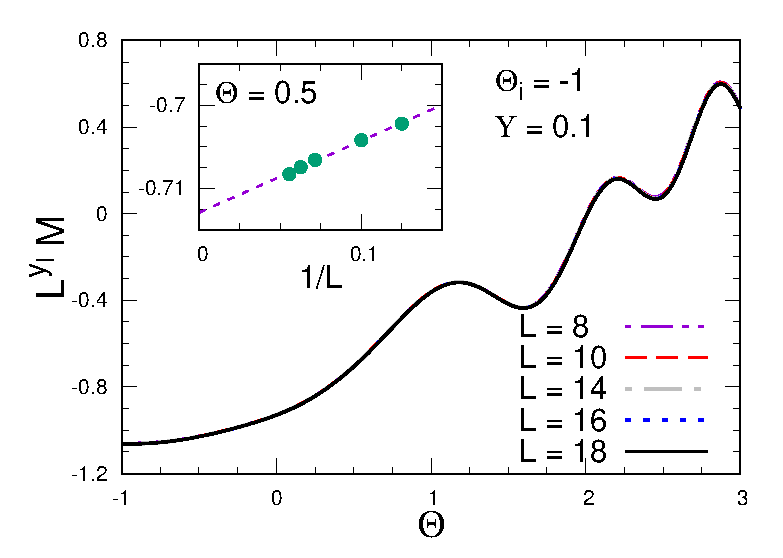
\includegraphics[width=0.65\columnwidth]{imm/IQY01ThX.eps}
  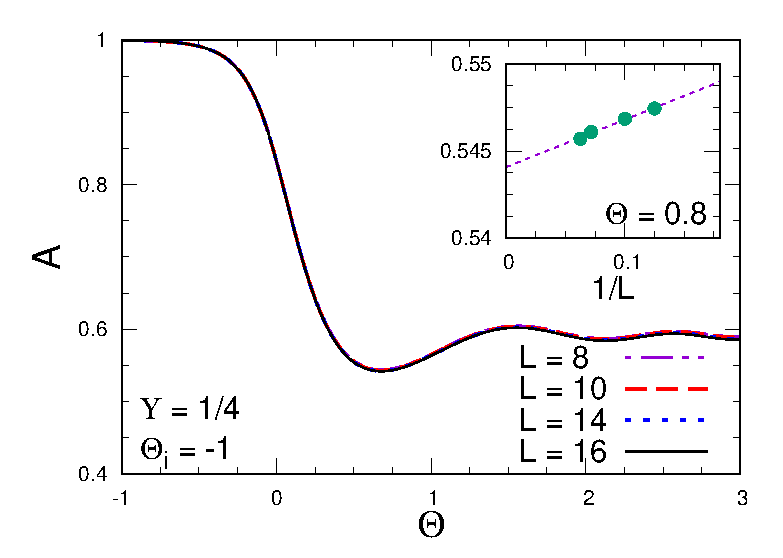
\includegraphics[width=0.65\columnwidth]{imm/IQY14ThA.eps}
  \caption{Dynamic FSS of the quantum Ising chain along the one-way KZ
    protocol at fixed $\Theta_i\equiv w_i L^{y_w}$.  We show results
    for the adiabaticity function $A(t,t_s,w_i,L)$ at fixed
    $\Upsilon=t_s/L^\zeta=1/4$ and $\Theta_i=-1$ up to $L=16$ (bottom)
    and the longitudinal magnetization $M(t,t_s,w_i,L)$ at fixed
    $\Upsilon=1/10$ and $\Theta_i=-1$ up to $L=18$ (top), versus
    $\Theta = t/t_s^\kappa$. The exponents $y_w$, $\zeta$, and
    $\kappa$ are reported in Eq.~(\ref{qisiexps}).  The approach to
    the large-$t_s$ asymptotic behavior is globally characterized by
    $O(1/L)$ corrections (apart from small superimposed wiggles), see
    for example the inset of the figures (where the line is drawn to
    guide the eyes).  }
  \label{dfssthetai}
\end{figure}


\begin{figure}[!htb]
\centering
  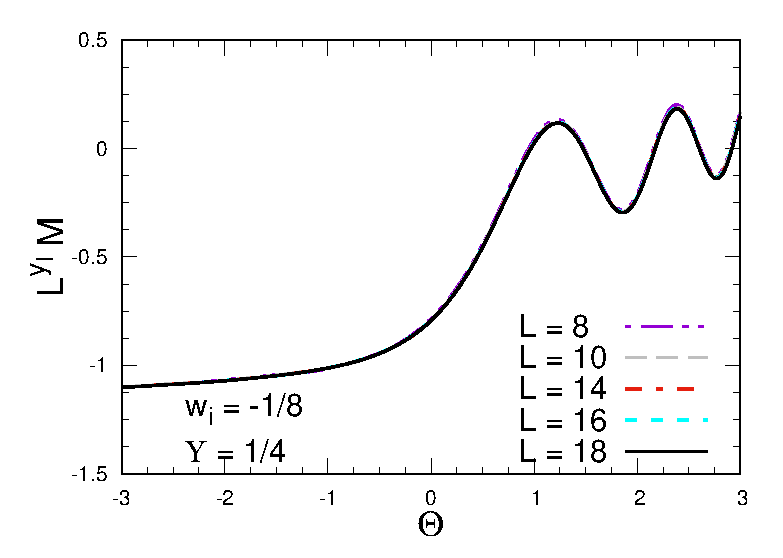
\includegraphics[width=0.65\columnwidth]{imm/IQY14W18X.eps}
  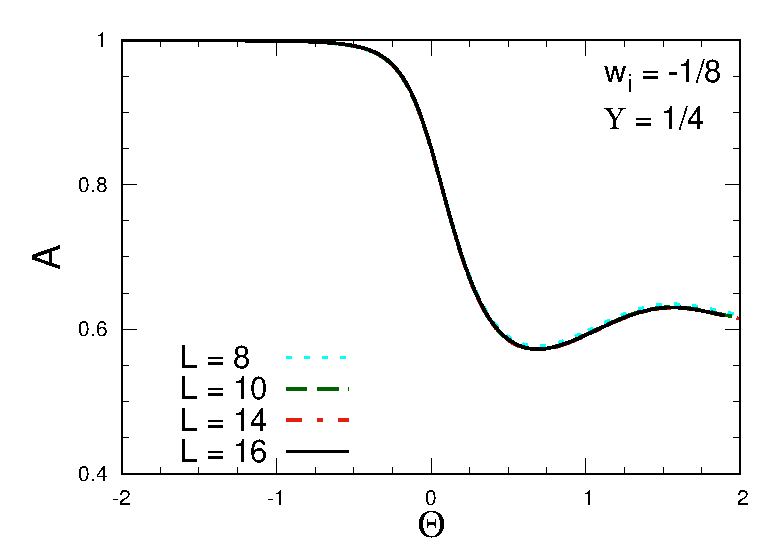
\includegraphics[width=0.65\columnwidth]{imm/IQY14W18A.eps}
  \caption{ Dynamic FSS of the quantum Ising chain along the one-way
    KZ protocol at fixed $w_i<0$.  We show the adiabaticity function
    $A(t,t_s,w_i,L)$ up to $L=16$ (bottom) and the longitudinal
    magnetization $M(t,t_s,w_i,L)$ up to $L=18$ (top), at fixed
    $\Upsilon=1/4$ and $w_i=-1/8$, versus $\Theta$. As explained in
    the text, the scaling behavior emerging at fixed $w_i<0$ matches
    that obtained in the $\Theta_i\to -\infty$ limit.}
  \label{dfsswi}
\end{figure}

The numerical analyses of quantum Ising chains (\ref{qisingmodel})
with a time-dependent longitudinal field is based on exact
diagonalization. The corresponding Schr\"odinger equation is solved
using a $4^{\rm th}$ order Runge-Kutta method. This approach allows us
to compute the out-of-equilibrium dynamics up to lattice size
$L\approx 16$, which, as we shall see, turns out to be sufficient to
achieve substantial evidence of the dynamic FSS outlined in the
previous sections.



We want to check the dynamic FSS put forward in Sec.~\ref{qfssoneway}.
In the case of the quantum 1D Ising model (\ref{isichoice}), the
exponents entering the definitions of the scaling variables
(\ref{KZscavar}) are 
\begin{equation}
y_w = 15/8\,,\qquad \zeta = 23/8\,,
\qquad \kappa = 8/23\,.
\label{qisiexps}
\end{equation}
Some results for the one-way protocol are reported in
Figs.~\ref{dfssthetai} and \ref{dfsswi}, respectively for the
adiabaticity function, defined in Eq.~(\ref{adtfunc}), and the
longitudinal magnetization, defined in Eq.~(\ref{magnt}), at fixed
$\Theta_i$ and $w_i$, for lattice sizes up to $L=16$ and $L=18$
respectively (this difference is due to the fact that the computation
of the adiabaticity function is heavier).  Although the system sizes
of the available results are only moderately large, we clearly observe
a collapse toward asymptotic scaling curves, thus a robust evidence of
the dynamic FSS outlined in Sec.~\ref{qfssoneway}.  In particular, the
dynamic FSS emerging from the data at fixed $w_i<0$ turns out to be
independent of the actual fixed value $w_i<0$, as predicted by the
scaling arguments reported in Sec.~\ref{qfssoneway} (in
Fig.~\ref{dfsswi} we only show results for $w_i=-1/8$, but we have
explicitly checked the independence of $w_i<0$ of the scaling
curves). We note that, as expected, the adiabaticity function
significantly drops crossing the quantum transition at finite values
of $\Upsilon$, while it remains close to one, i.e. the value
corresponding to adiabatic evolutions, for large values of $\Upsilon$.
We also  note that the data show that the convergence to the
asymptotic dynamic FSS is globally consistent with $O(1/L)$
corrections (apart from superimposed wiggles).


Analogous results are obtained for the quantum Kitaev wire, with
driving chemical potential.  The corresponding exponents,
cf. Eq.~(\ref{KZexps}), entering the definitions of the scaling
variables (\ref{KZscavar}), are
\begin{equation}
y_w = 1, \qquad \zeta = 2\,,\qquad \kappa =
1/2\,.
\label{kexps}
\end{equation}
The simpler {\em integrable} nature of the quantum Kitaev wire
(\ref{kitaev2}) allows us to easily consider much larger systems, up
to $L\approx 10^3$, using standard procedures after Fourier
transforming to the momentum space. Again the resulting data (not
shown) for the adiabaticity function, energy surplus, particle
density, and the two-point functions, cf. Eq.~(\ref{eq:corr}), nicely
support the dynamic FSS outlined in Sec.~\ref{qfssoneway}, see also
Ref.~\cite{rossini2021coherent}.



\subsection{Along the classical round-trip KZ protocol}
\label{clroundtrip}


\begin{figure}[!htb]
\centering
  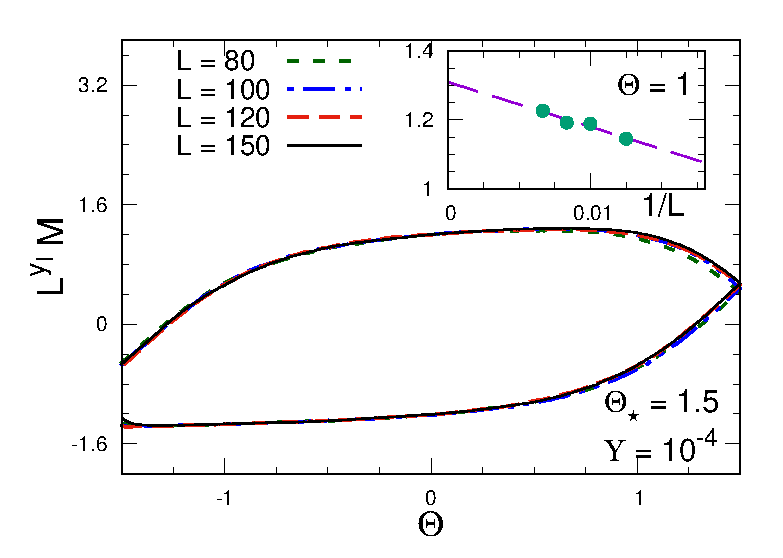
\includegraphics[width=0.65\columnwidth]{imm/isC2DT15Y104.eps}
  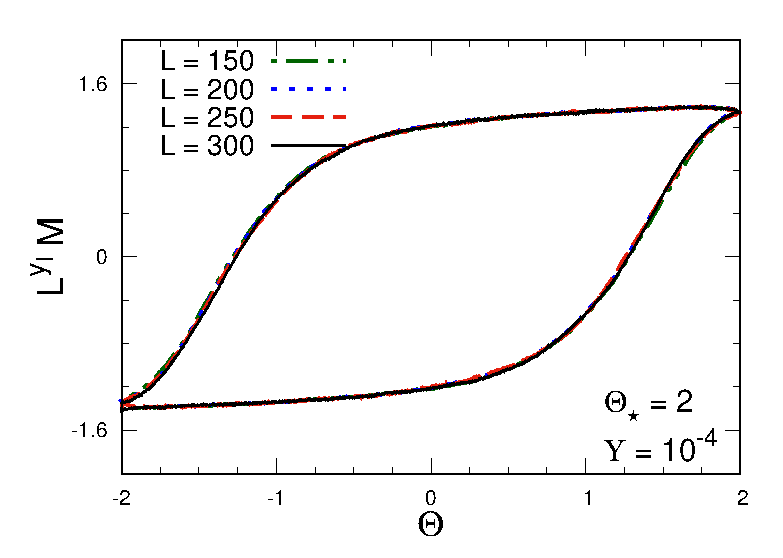
\includegraphics[width=0.65\columnwidth]{imm/isC2DT2Y104.eps}
  \caption{ Dynamic FSS behavior of $M(t,t_s,w_\star,L)$ for classical
    Ising model along the round-trip KZ protocol. Data are obtained at
    fixed $\Upsilon=10^{-4}$, and fixed $\Theta_\star = 1.5$ (top) and
    $\Theta_\star = 2$ (bottom), and are plotted versus $\Theta=w(t)
    t_s^{1-\kappa}$. The convergence is globally consistent with a
    $1/L$ behavior, see for example the inset of the top figure.  The
    values of the exponents $y_w$, $\zeta$, and $\kappa$ are reported
    in Eq.~(\ref{clisiexps}). Statistical errors are typically smaller
    than the thickness of the lines.}
  \label{roundtripM}
\end{figure}


\begin{figure}[!htb]
\centering
    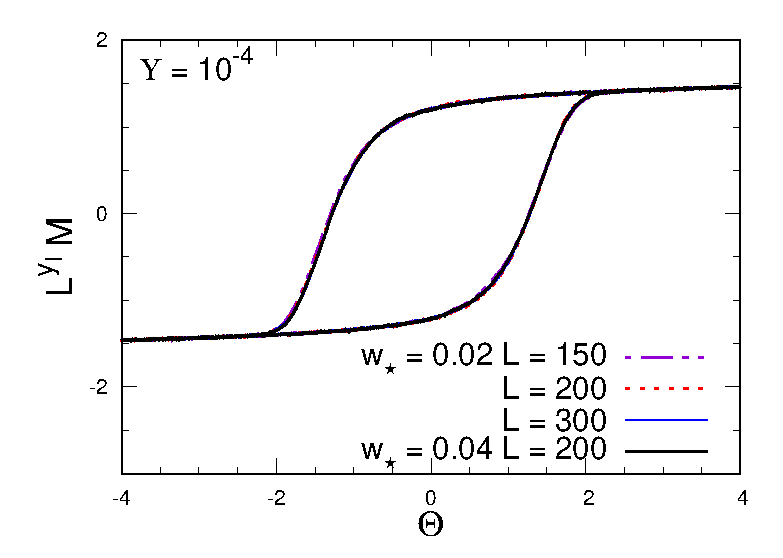
\includegraphics[width=0.65\columnwidth]{imm/isC2Dw002Y104.eps}
  \caption{ Dynamic FSS behavior of $M(t,t_s,w_\star,L)$ for the
    classical 2D Ising model along the round-trip KZ protocol for
    fixed $\Upsilon=10^{-4}$, and fixed $w_\star = 0.02$ and $w_\star
    = 0.04$. Statistical errors are typically smaller than the
    thickness of the lines. These results clearly support the
    predicted scaling behaviors, see Sec.~\ref{cfssKZroundtrip}, and
    their independence of the finite value of $w_\star>0$.  }
  \label{roundtripMW}
\end{figure}


\begin{figure}[!htb]
\centering
    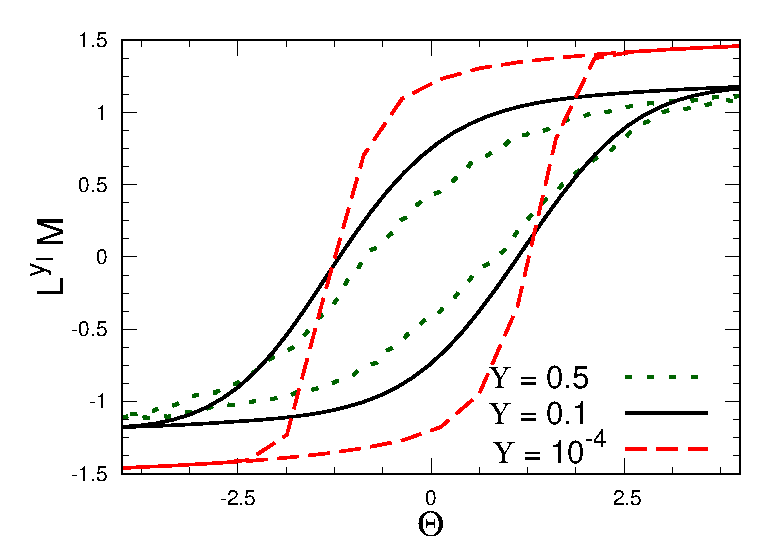
\includegraphics[width=0.65\columnwidth]{imm/isC2DL50.eps}
    \caption{Histeresis curves of the magnetization
      $M(t,t_s,w_\star,L)$ for the classical 2D Ising model along the
      round-trip KZ protocol for various values of fixed $\Upsilon$.
      They confirm that the hysteresis area decreases as $\Upsilon$
      increases. The curve for $\Upsilon=10^{-4}$ is taken from the
      data shown in Fig.~\ref{roundtripMW}, those for $\Upsilon=0.1$
      and $\Upsilon=0.5$ are obtained from simulations for $L=50$,
      whose size is already sufficient to provide a good approximation
      of the asymptotic large-$L$ scaling curves (note that Monte
      Carlo simulations becomes more demanding with increasing
      $\Upsilon$).}
  \label{roundtripMW2}
\end{figure}



The numerical analysis of the classical Ising model is based on
standard Monte Carlo simulations based on local Metropolis upgrading
procedures~\cite{Metropolis:1953am}, which provide a purely
relaxational dynamics without conserved quantities, that is model A
according to the standard classification reported in
Ref.~\cite{HH-77}.  The time unit of this dynamics is represented by a
global sweep of upgradings of all $L\times L$ spin variables. We
perform the single-site update sequentially, moving from one site to
one of its neighbours in a typewriter fashion.  The results along the
time-dependent protocols are obtained by averaging over a sample of
trajectories (tipically of order $10^3$), starting from an ensemble of
thermalized configurations at the initial parameter values. Also in
this case relatively large systems can be simulated, typically for
$L\gtrsim 10^2$.



The dynamic scaling arising from the one-way protocol is quite
analogous to that observed at quantum transitions, with corresponding
scaling behaviors, characterized by the static Ising critical exponents
supplemented by the purely relaxational dynamic exponent $z = 2.167(1)$.
The corresponding relevant exponents, cf. Eq.~(\ref{KZexps}), entering
the definitions of the scaling variables (\ref{KZscavar}), are
\begin{equation}
  y_w = 15/8\,,\quad \zeta = 4.0420(1)\,,\quad
  \kappa = 0.5361(1)\,.
  \label{clisiexps}
  \end{equation}
In the following we only report results for the round-trip KZ protocols,
taking also into account that its first part is equivalent to the
one-way KZ protocol.

The dynamic scaling behavior of the magnetization,
cf. Eq.~(\ref{genOscart}), is fully supported by the data reported in
Fig.~\ref{roundtripM}, for a fixed $\Upsilon=10^{-4}$ and two
different values of $\Theta_\star$.  Analogous results are obtained
for other values of $\Upsilon$.  As expected the round-trip cycle does
not close the curves for finite values of $\Upsilon$ and
$\Theta_\star$, see Eq.~(\ref{disacy}), leaving a finite gap between
the initial and final values of the cycle, i.e.
\begin{equation}
  {\cal M}^{(b)}(\Upsilon,-\Theta_{\star},\Theta_\star) -
  {\cal M}^{(a)}(\Upsilon,-\Theta_{\star},\Theta_\star)>0\,,
  \label{disacy2}
\end{equation}
which becomes smaller and smaller with increasing $\Theta_\star$.

As argued in Sec.~\ref{cfssKZroundtrip}, the outward and return
trajectories close in the large-$\Theta_\star$ limit, and therefore
for finite $w_\star>0$, giving rise to critical hysteresis phenomena.
This is clearly demonstrated by the results shown in
Fig.~\ref{roundtripMW} for two different finite values of $w_\star>0$,
whose scaling curves coincide. The outward and return curves for large
$|\Theta|$ tend to coincide, differing only within a finite interval
around $\Theta=0$, which becomes smaller and smaller with increasing
$\Upsilon$, and vanishes in the adiabatic limit
$\Upsilon\to\infty$. Such a dependence on $\Upsilon$ is demonstrated
by the curves reported in Fig.~\ref{roundtripMW2} showing the
magnetization hysteresis for various values of $\Upsilon$. They
confirm the scaling law (\ref{IAsca}) of the hysteresis area. Morever,
the data at small values of $\Upsilon$ hint at a convergence to a
constant for $\Upsilon\to 0$, which corresponds to the infinite-volume
limit.

As we shall see, these peculiar behaviors of round-trip protocols
developing scaling hysteresis do not have a quantum counterpart, being
strictly connected with the thermalizing relaxational dynamics of
classical models.


We also stress that the above hysteresis scenario arises from the
round-trip protocols between phases with short-ranged
correlations. More complicated situations are expected to occur when
round-trip protocols involve ordered phases, where coarsening
phenomena may drastically change the picture, in particular
along the return trip, in the large-$\Theta_\star$ limit.

\subsection{Along the quantum round-trip KZ protocol}
\label{qroundtrip}

\subsubsection{Scaling for finite $\Theta_\star$}
  \label{scafinthetastar}

\begin{figure}[!htb]
\centering
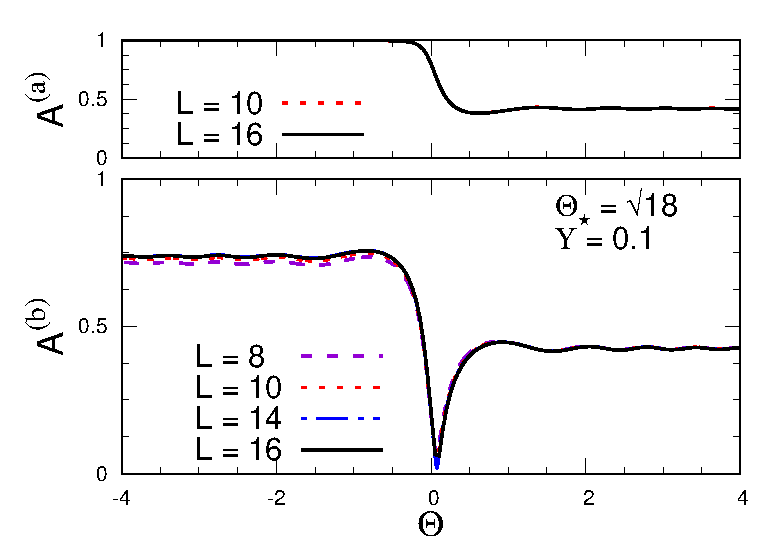
\includegraphics[width=0.65\columnwidth]{imm/headIQMY01ThA.eps}
\caption{ Round-trip dynamic FSS of the quantum Ising chain,
  cf. Eq.~(\ref{isichoice}, for a finite $\Theta_\star$.  We show
  results for the adiabaticity function $A(t,t_s,w_\star,L)$ at fixed
  $\Upsilon = t_s/L^\zeta= 0.1$ and $\Theta_\star = w_\star
  L^{1-\kappa}=3\sqrt{2}$, for the outward (top) and return (bottom)
  branches of the round-trip KZ protocol, versus
  $\Theta=w(t)L^{1-\kappa}$, for various size $L$ up to $L=16$.  The
  values of the exponents $y_w$, $\zeta$, and $\kappa$ are reported in
  Eq.~(\ref{qisiexps}).  The shown results clearly support the dynamic
  scaling behavior given in Eq.~(\ref{asca3}).  }
    \label{roundtripA}
\end{figure}


\begin{figure}[!htb]
\centering
  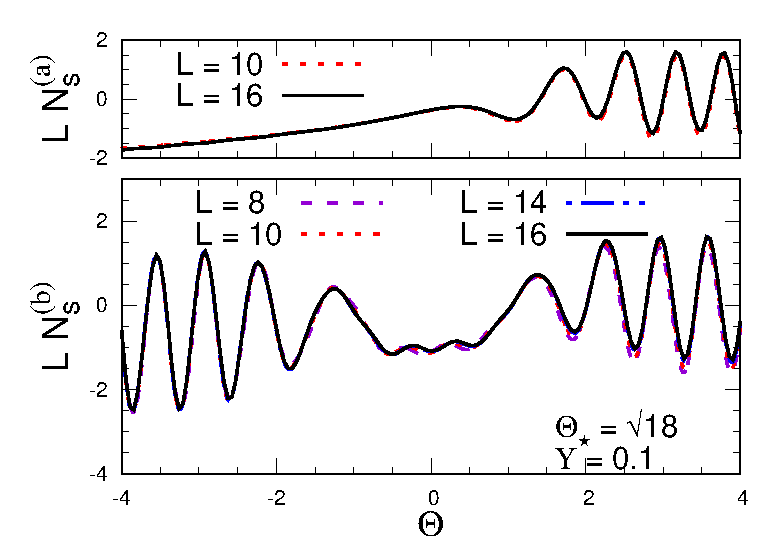
\includegraphics[width=0.65\columnwidth]{imm/headIQMY01ThZ.eps}
  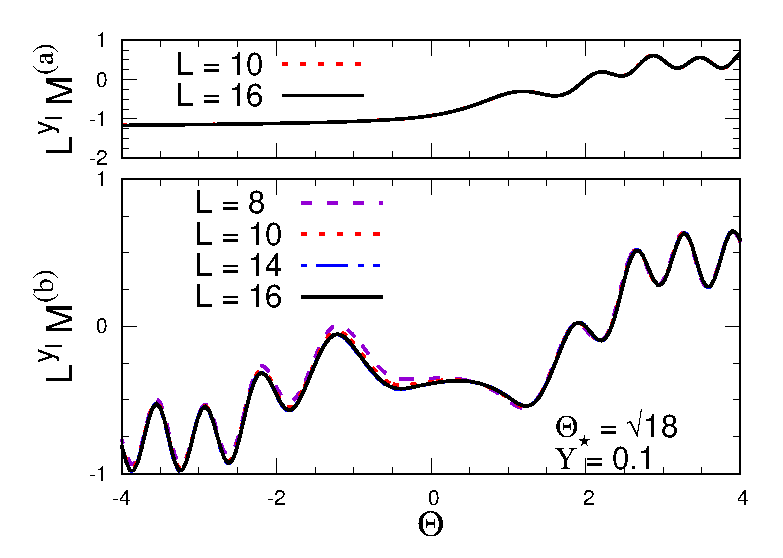
\includegraphics[width=0.65\columnwidth]{imm/headIQMY01ThX.eps}
  \caption{ Round-trip dynamic FSS of the longitudinal magnetization
    $M(t,t_s,w_\star,L)$ (bottom figure) and subtracted transverse
    magnetization $N_s(t,t_s,w_\star,L)$ (top figures),
    cf. Eq.~(\ref{subdef}), in the quantum Ising chain at fixed
    $\Upsilon=0.1$ and $\Theta_\star = 3\sqrt{2}$, for the outward
    (top) and return (bottom) branches of the round-trip KZ protocol,
    versus $\Theta$, for various size $L$ up to $L=16$.  The results
    clearly support the dynamic scaling behavior given in
    Eq.~(\ref{genOscart}).}
  \label{roundtripMN}
\end{figure}


\begin{figure}[!htb]
\centering
  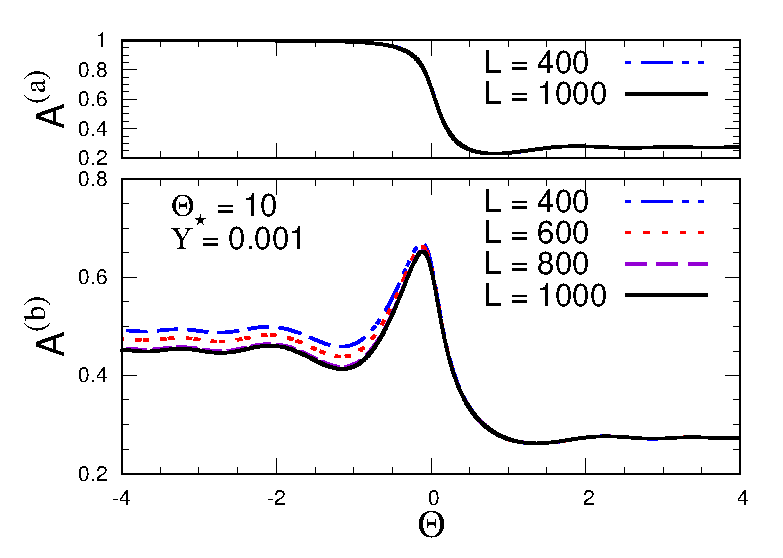
\includegraphics[width=0.65\columnwidth]{imm/headKITY0001Th10A.eps}
  \caption{ Round-trip dynamic FSS within the quantum Kitaev wire for
    a finite $\Theta_\star$.  We show results for the adiabaticity
    function $A(t,t_s,w_\star,L)$ at fixed $\Upsilon =t_s/L^\zeta =
    0.001$ and $\Theta_\star = w_\star L^{1-\kappa}=10$, for the
    outward (top) and return (bottom) branches of the round-trip KZ
    protocol, versus $\Theta=w(t)L^{1-\kappa}$, for various size $L$
    up to $L=1000$.  The values of the exponents $y_w$, $\zeta$, and
    $\kappa$ are reported in Eq.~(\ref{kexps}).  The numerical results
    clearly support the dynamic scaling behavior given in
    Eq.~(\ref{asca3}).}
  \label{roundtripdfssA}
\end{figure}

\begin{figure}[!htb]
\centering
  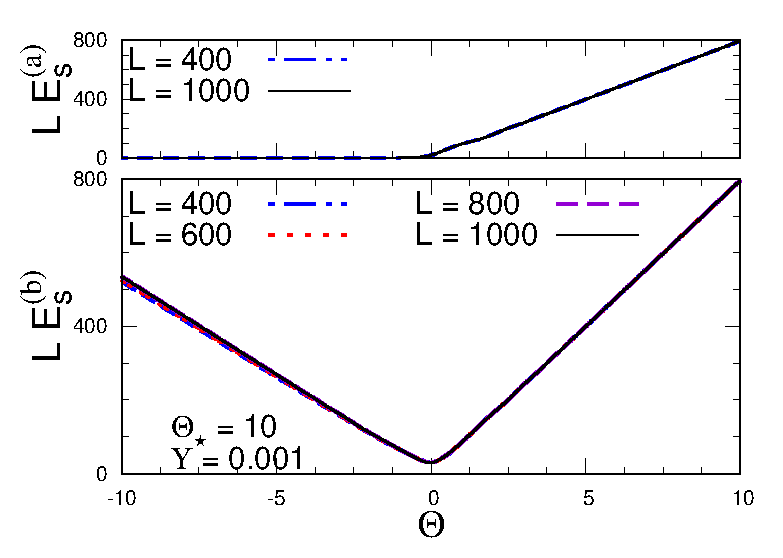
\includegraphics[width=0.65\columnwidth]{imm/headKITY0001Th10E.eps}
  \caption{ Round-trip dynamic FSS within the quantum Kitaev wire for
    a finite $\Theta_\star$.  We show results for the surplus energy
    $E_s(t,t_s,w_\star,L)$ defined in Eq.~(\ref{etdiff}), at $\Upsilon
    =t_s/L^\zeta = 0.001$, and $\Theta_\star = w_\star
    L^{1-\kappa}=10$, for the outward (top) and return (bottom)
    branches of the round-trip KZ protocol, versus
    $\Theta=w(t)L^{1-\kappa}$, for various size $L$ up to $L=1000$.
    The results clearly support
  the dynamic scaling behavior given in Eq.~(\ref{esca3}).
    }
  \label{roundtripdfssE}
\end{figure}


\begin{figure}[!htb]
\centering
  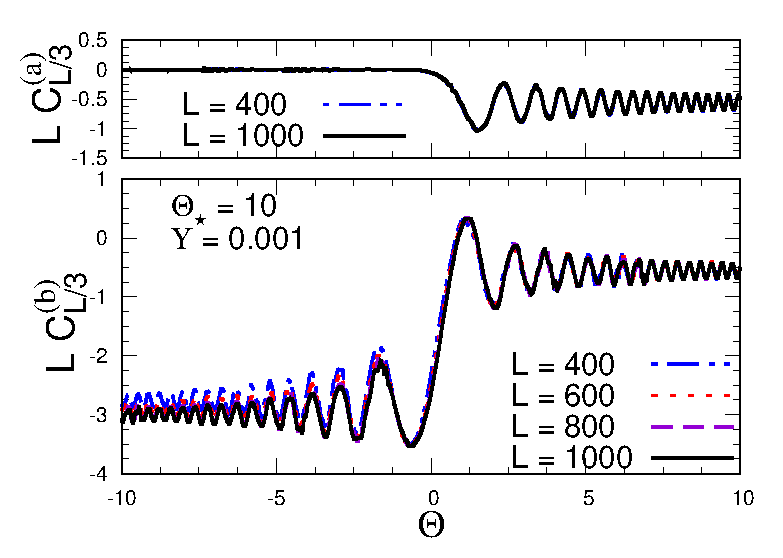
\includegraphics[width=0.65\columnwidth]{imm/headKITY0001Th10C.eps}
  \caption{ Round-trip dynamic FSS within the quantum Kitaev wire for
    a finite $\Theta_\star$.  We show results for the two-point
    function $C(x,t,t_s,w_\star,L)$, cf. Eq.~(\ref{eq:corr}), at fixed
  $X=x/L=1/3$, $\Upsilon =t_s/L^\zeta = 0.001$, and $\Theta_\star =
  w_\star L^{1-\kappa}=10$, for the outward (top) and return (bottom)
  branches of the round-trip KZ protocol, versus
  $\Theta=w(t)L^{1-\kappa}$, for various size $L$ up to $L=1000$.
  }
  \label{roundtripdfssC}
\end{figure}




To begin with, we show results for round-trip KZ protocols for the
quantum Ising chain, cf. Eq.~(\ref{isichoice}), when keeping
$\Theta_\star$ finite, see Figs.~\ref{roundtripA}
and \ref{roundtripMN}, respectively for the adiabaticity function, the
longitudinal and transverse magnetizations.  Analogous results are
obtained for other values of $\Upsilon$ and $\Theta_\star$. They
nicely support the scaling behaviors put forward in
Sec.~\ref{qfssKZroundtrip}.  Analogous results are obtained for the
quantum Kitaev wire, cf. Eq.~(\ref{kitchoice}), see for example the
results shown in Figs.~\ref{roundtripdfssA}, \ref{roundtripdfssE}, and
\ref{roundtripdfssC}, respectively for the adiabaticity function, the
surplus energy $E_s$ defined in Eq.~(\ref{etdiff}), and the two point
function defined in Eq.~(\ref{eq:corr}). They nicely support the
dynamic FSS at fixed finite $\Theta_\star$.



\subsubsection{The limit $\Theta_\star\to\infty$}
  \label{scafinthetastarinf}

\begin{figure}[!htb]
\centering
  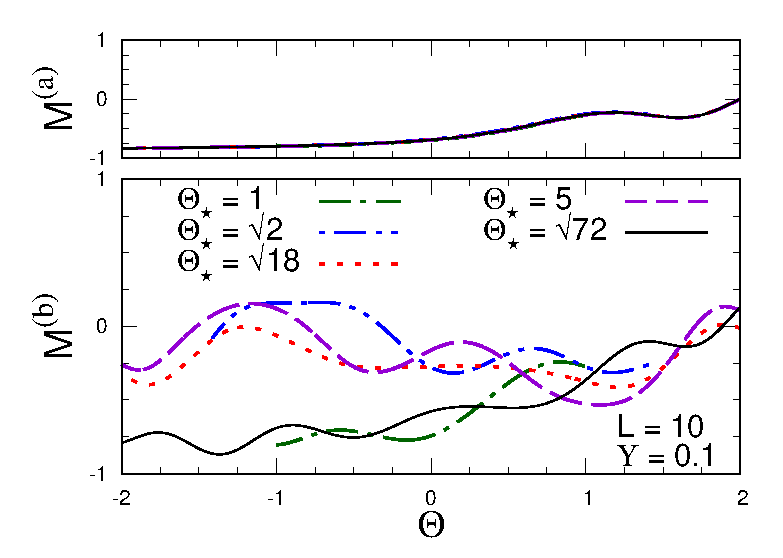
\includegraphics[width=0.65\columnwidth]{imm/headDiffThsY01L10X.eps}
 \caption{ Behavior of $M(t,t_s,w_\star,L)$ for fixed $L = 10$,
   $\Upsilon = 0.1$ for the one way trip (top figure) and for the
   return trip (bottom figure), versus $\Theta$, for various
   $\Theta_\star$ up to $\Theta_\star = 6\sqrt{2}$.  We note that
   along the outward path the convergence is large-$\Theta_\star$
   convergence is rapid (it is essentially related to the convergence
   with respect to $\Theta_i=-\Theta_\star$ of the one-way protocol),
   along the return path the curves do not appear to approach a
   large-$\Theta_\star$ limit.}
  \label{diffThetaStar}
\end{figure}


We now discuss the large-$\Theta_\star$ limit, or equivalently the
case in which we keep $w_\star>0$ fixed in the round-trip protocols.
This limit turns out to be quite problematic in quantum round-trip KZ
protocols.

  
Some hints at the absence of a well defined large-$\Theta_\star$ limit
of the dynamic scaling behavior are shown by the plots of
Fig.~\ref{diffThetaStar} reporting the longitudinal magnetization of a
quantum Ising system of size $L=10$ for various $\Theta_\star$, whose
return paths do not show any apparent convergence when increasing
$\Theta_\star$.



\begin{figure}[!htb]
\centering
  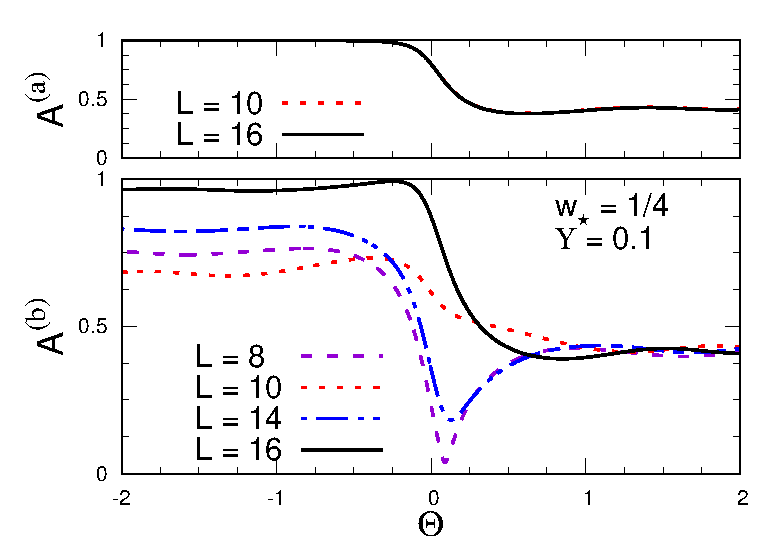
\includegraphics[width=0.65\columnwidth]{imm/headIQMY01W025A.eps}
  \caption{ The adiabaticity function $A(t,t_s,w_\star,L)$ of quantum
    Ising chains along round-trip protocols, for fixed $\Upsilon =
    0.1$ and $w_\star = 1/4$, for the outward (top) and return
    (bottom) branches of the round-trip protocol, versus $\Theta$, for
    various size $L$ up to $L=16$.  }
  \label{roundtripAW}
\end{figure}


\begin{figure}[!htb]
\centering
  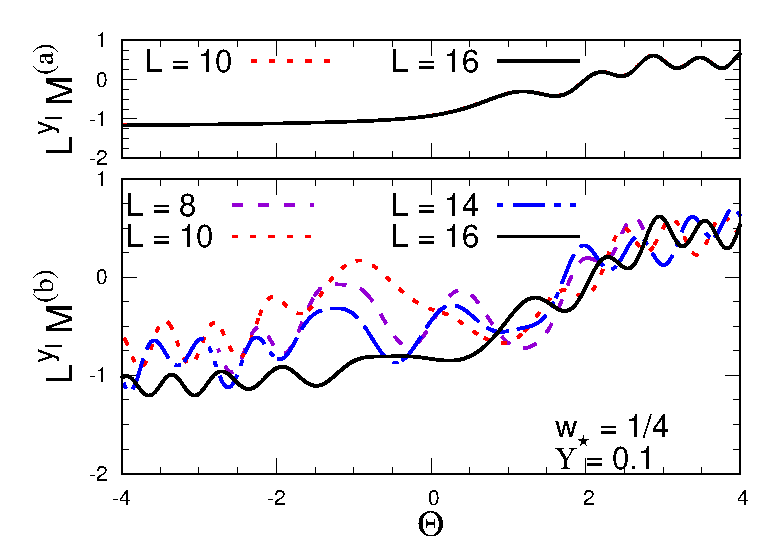
\includegraphics[width=0.65\columnwidth]{imm/headIQMY01W025X.eps}
 \caption{ The longitudinal magnetization $M(t,t_s,w_\star,L)$ along
   the round-trip protocol, for fixed $w_\star = 1/4$, $\Upsilon =
   0.1$ for the outward (top) and return (bottom) branches of the
   round-trip protocol, versus $\Theta$, for various size $L$ up to
   $L=16$.  }
  \label{roundtripMxW}
\end{figure}


%\begin{figure}[!htb]
%\centering
%  \includegraphics[width=0.65\columnwidth]{imm/headIQMY01W025Z.eps}
% \caption{ The subtracted transverse magnetization
%   $N_s(t,t_s,w_\star,L)$ along the round-trip protocol, for fixed
%   $w_\star = 1/4$, $\Upsilon = 0.1$ for the outward (top) and return
%   (bottom) branches of the round-trip protocol, versus $\Theta$, for
%   various size $L$ up to $L=16$.  }
%  \label{roundtripMzW}
%\end{figure}





\begin{figure}[!htb]
\centering
  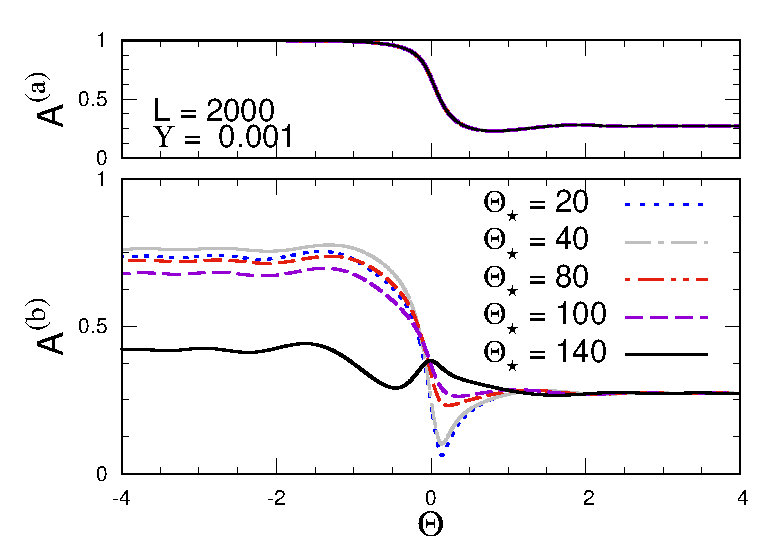
\includegraphics[width=0.65\columnwidth]{imm/headKITY0001L2000A.eps}
 \caption{The adiabaticity function $A(t,t_s,w_\star,L)$ for the
   quantum Kitaev wire at $L=2000$ and $\Upsilon = 0.001$ for the
   outward (top) and return (bottom) branches of the round-trip KZ
   protocol, versus $\Theta$, for various $\Theta_\star$ up to
   $\Theta_\star = 140$.  We note that along the outward path the
   convergence is large-$\Theta_\star$ convergence is rapid (it is
   essentially related to the convergence with respect to
   $\Theta_i=-\Theta_\star$ in the one-way KZ protocol), along the
   return path the curves do not appear to approach a
   large-$\Theta_\star$ limit.}
  \label{diffThetaStarA}
\end{figure}

The return trajectories keeping $w_\star>0$ fixed do not show evidence
of convergence in the large-$L$ dynamic scaling limit.  This is shown
by the curves of the adiabaticity function along the return branch of
the round-trip protocol, see Fig.\ref{roundtripAW}, for $w_\star=1/4$
and $\Upsilon=0.1$.  While convergence is clearly observed along the
outward part, as expected because the one-way protocol showed a well
defined limit in the large-$|\Theta_i|$ limit, the return pattern does
not show a stable convergence pattern. The same behavior is also shown
by the longitudinal and transverse magnetizations $M$ and $N$, see for
example Fig.~\ref{roundtripMxW}.  Analogous results are also obtained
for the quantum Kitaev wire, see Fig.~\ref{diffThetaStarA}, where we
report results for the adiabaticity function at $\Upsilon=0.001$ and
various large values of $\Theta_\star$, for a large lattice size
$L=2000$.

Actually, such an instability appears quite similar to that emerging
in analogous round-trip protocols within two-level systems.  They are
discussed in App.~\ref{LZlike}. Similarly to the 
Landau-Zener problem~\cite{zener1932non}, we consider a time-dependent two-level
Hamiltonian
\begin{equation}
  H_{2\ell}(t) = - \beta(t) \sigma^{(3)}
  + {\Delta\over 2} \sigma^{(1)}\,,
\label{hrdef2}
\end{equation}
where $\Delta$ is a constant, 
\begin{eqnarray}
  \beta(t) = {{\cal T}(t)\over t_s}\quad
       {\rm for}\;\; t_i=-t_\star \le t \le 3t_\star\,,
\label{betadef}
\end{eqnarray}
and $ {\cal T}(t) = t_\star - |t-t_\star|$ is the triangular
function. The quantities $\tau={\cal T}(t)/\sqrt{t_s}$ and
$\tau_\star=t_\star/\sqrt{t_s}$ play the same role of the scaling
variables $\Theta$ and $\Theta_\star$ describing the round-trip KZ
protocols in quantum many-body systems. The corresponding
Schr\"odinger functions can be analytically solved in terms 
of parabolic cylinder functions $D_\nu(x)$~\cite{vitanov1996landau}, see
App.~\ref{LZlike}.

The resulting behavior of the expectation values of $\sigma^{(3)}$ and
the adiabatic function show that the large-$\tau_\star$ limit is
problematic, being characterized by large $O(1)$ oscillations with
frequencies increasing proportionally to $\tau_\star$, roughly. See
App.~\ref{LZlike} for details.  They turn out to be related to the
rapid changes of the relative phase between the relevant states of the
two-level system at the extremal values $\tau=\tau_\star$ when
$\tau_\star$ becomes large, increasing as $\tau_\star^2$. Since the
quantum evolution along the return trajectory turns out to be very
dependent on such phase, it becomes extremely sensitive to the value
of $\tau_\star$, showing analogous oscillations. As a consequence, the
value of all observables along the return trajectory, from
$\tau=\tau_\star$ down to the return point $\tau = - \tau_\star$, do
not show a well defined limit for $\tau_\star\to\infty$.  The size of
the oscillations depend on the value of the scaling variable
$\Upsilon$, and tend to be suppressed in the adiabatic limit
$\Upsilon\to\infty$.

\begin{figure}[!htb]
\centering
  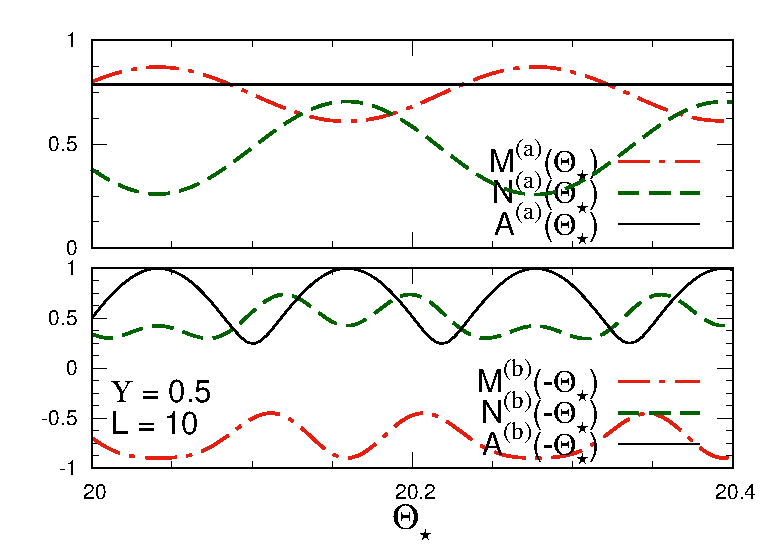
\includegraphics[width=0.45\columnwidth]{imm/diffThstaru50s20l10.eps}
  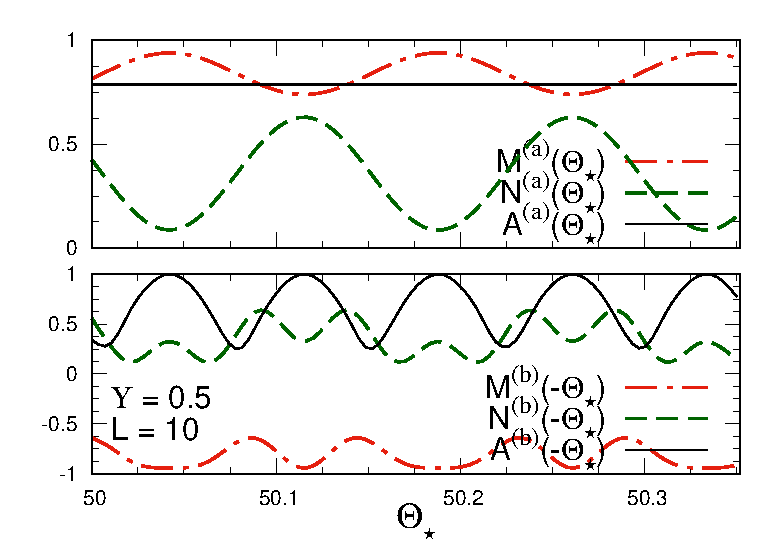
\includegraphics[width=0.45\columnwidth]{imm/diffThstaru50s50l10.eps}
 \caption{ Results for $M,\, N$ and $A$ for fixed $L = 10$, $\Upsilon
   = 0.5$ versus $\Theta_\star$, close to $\Theta_\star = 20$ (top
   figure) and $\Theta_\star = 50$ (bottom figure). In each figure,
   the top plot the values of $M^{(a)}$, $N^{(a)}$ and $A^{(a)}$ at
   the end of the outward branch, corresponding to
   $\Theta=\Theta_\star$, while the bottom plot shows the values of
   $M^{(b)}$, $N^{(b)}$ and $A^{(b)}$ at the end of the return branch,
   corresponding to $\Theta=-\Theta_\star$. The comparison of the top
   and bottom figures show that the oscillations tend to become more
   frequent with increasing $\Theta_\star$ (note that the interval of
   the abscissa is different).  Analogous results are obtained for
   other values of $\Upsilon$.}
  \label{roundtripDiffTheta}
\end{figure}

%\begin{figure}[!htb]
%  \centering
%  \includegraphics[width=0.65\columnwidth]{imm/diffThstaru10s25l10.eps}
%  \includegraphics[width=0.65\columnwidth]{imm/diffThstaru10s50l10.eps}
% \caption{ Results for $M,\, N_s$ and $A$ for fixed $L = 10$,
%   $\Upsilon = 0.1$ versus $\Theta_\star$, close to $\Theta_\star =
%   20$ (top figure) and $\Theta_\star = 50$ (bottom figure). In each figure,
%   the top plot shows the one way trip, while the bottom plot shows
%   the return trip.   }
%  \label{roundtripDiffTheta2}
%\end{figure}



\begin{figure}[!htb]
\centering
%  \includegraphics[width=0.65\columnwidth]{imm/diffThstaru0001T35l40.eps}
   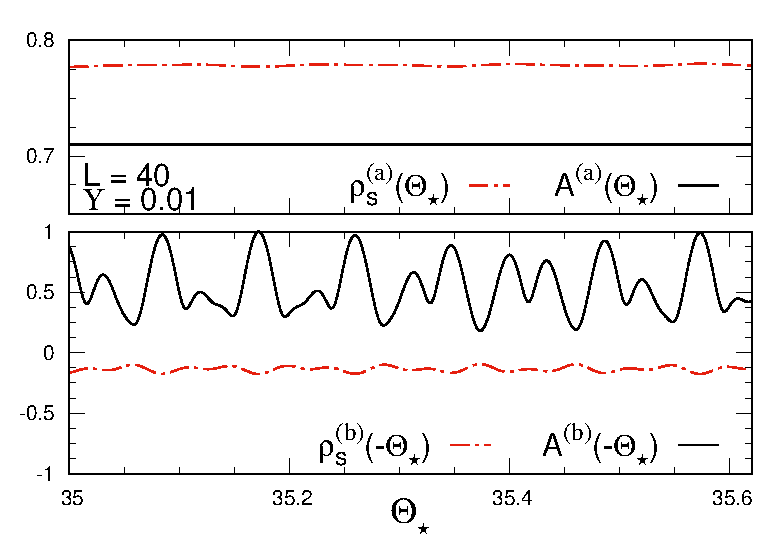
\includegraphics[width=0.45\columnwidth]{imm/diffThstaru001T35l40.eps}
  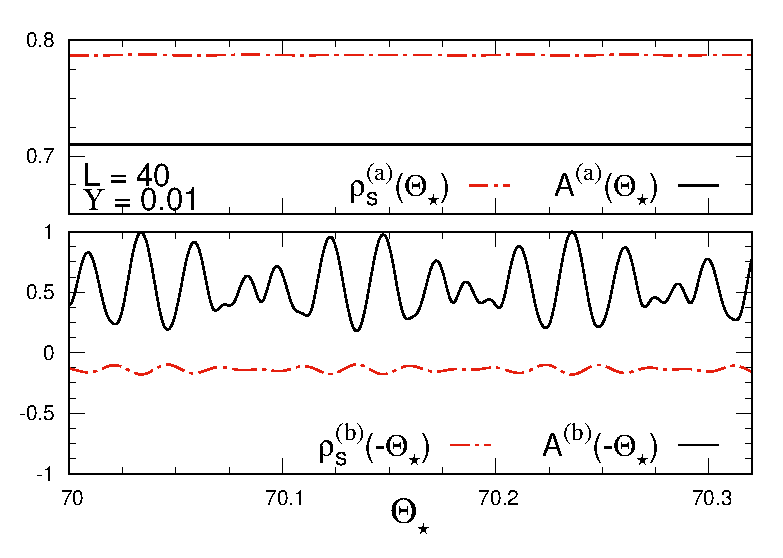
\includegraphics[width=0.45\columnwidth]{imm/diffThstaru001T70l40.eps}
  \caption{ Behavior of the subtracted particle density $\rho_s$,
    cf. Eq.~(\ref{rhot}), and the adiabaticity function $A$ for the
    Kitaev wire, for fixed $L = 40$, $\Upsilon = 0.01$ versus
    $\Theta_\star$, close to $\Theta_\star = 70$ (bottom figure) and
    $\Theta_\star=35$ (top figure).  In each figure, the top plot the
    values of $\rho_s^{(a)}$ and $A^{(a)}$ at the end of the outward
    branch, corresponding to $\Theta=\Theta_\star$, while the bottom
    plot shows the values of $\rho_s^{(b)}$ and $A^{(b)}$ at the end
    of the return branch, corresponding to $\Theta=-\Theta_\star$.
    Again, the comparison of the top and bottom figures show that the
    oscillations tend to become more frequent with increasing
    $\Theta_\star$.  }
  \label{roundtripDiffThetaAR}
\end{figure}



We observe a similar behavior in the quantum many-body systems.  This
scenario is demonstrated by the results shown in
Fig.~\ref{roundtripDiffTheta}, where we report the values of $A$, $M$,
and $N_s$ at end of the outward branch and at the end of the return
branch for some interval of values of $\Theta_\star$, around large
values of $\Theta_\star$ and fixed $L=10$.  Similarly to the results
obtained for two-level model, the observables at the end of the
outward branch oscillate, with a frequency that becomes larger and
larger with increasing $\Theta_\star$, and the oscillations observed
after the whole cycle are strongly correlated to those at the end of
the first branch, doubling the frequency.  Analogous results are
obtained for other values of $\Upsilon$.  We also note that the
oscillations tend to be suppressed in the adiabatic
$\Upsilon\to\infty$ limit. We believe that this extreme sensitivity to
$\Theta_\star$ makes also problematic the large-$L$ limit after the
limit $\Theta_\star\to\infty$ shown by the numerical data.

Similar results are also obtained for the quantum Kitaev wire, see
Fig.~\ref{roundtripDiffThetaAR} where we show results for the
adiabaticity function and the particle density.  In this case the
values at the end of the outward way appear quite stable, but the
return way is characterized again by large (less regular) oscillations
with larger and larger frequencies with increasing $\Theta_\star$.


On the basis of the above results, we conclude that in quantum
many-body systems the large-$\Theta_\star$ limit of the dynamic KZ
scaling does not apparently exist along the return trajectories,
showing similarities with the behavior of two-level model
(\ref{hrdef2}) subject to round-trip protocols. We believe that this
issue deserves further investigation, for example addressing the
possibility of obtaining well defined scaling behavior after some
average procedures over the oscillations induced by large valyes of
$\Theta_\star$, to obtained a well defined large-$\Theta_\star$ limit.

However, we stress that the dynamic scaling behavior is nicely
observed when keeping $\Theta_\star$ fixed, even along the return
trajectory. This is related to fact that, when keeping $\Theta_\star$
fixed, the time scaling variable $\Theta$ remains finite, therefore
the time variable is always rescaled consistently with the time scale
of the equilibrium quantum transition, provided by the inverse gap at
the transition $\Delta \sim L^{-z} \sim \lambda^{-z}$. As a
consequence, the the variation of $w(t)$ gets limited within a small
interval $\delta_w$ around the transition, which becomes smaller and
smaller in the large-size limit, as $\delta_w \sim L^{-y_w}$.


%\section{First-Order Transition}
\label{rtripfoqt}

\subsection{Driving Protocol}


Under this analogy, as well as the Kibble-Zurek mechanism captures the defects 
density generated across the criticality from an initial equilibrium homogeneous state,
out-of-equilibrium finite-size scaling relations at the FOQT quantify the transition to the
first excited level during the driving from an initial (non-critical) ground state.
However, understanding whether similar scaling relations occur when the system is
driven across a quantum phase transition from an out-of-equilibrium configuration is 
still not clear. So far, results are limited to the recent Ref. [53], and yet unexplored
for FOQTs. This is the scope of this manuscript. Below, we
investigate the emergence of finite-size scaling behaviors
during a round-trip driving across the first-order point. As
result, we find that out-of-equilibrium scaling behaviors
are still observed (even after several passages across the
FOQT), although the associated scaling functions develops
a dependence on the details of the driving protocol at the
inversion time.



\subsection{Finite Size Scaling at FOQT}







\subsection{Effettive Description}




\subsection{Floquet Driving}




\subsection{Summary}



   \chapter{Dissipation}
\label{chp_diss}


\section{Introduction}

The analysis of open quantum many-body systems plays an important role in fundamental problems of quantum physics, such as quantum information, quantum computing, decoherence and condensed matter physics. The recent progress in the experimental techniques and the realizations of physical devices for quantum computing gives a further motivation to understand the general behavior of these open quantum systems. They involve a wide class of different specific issues as the study of the non-equilibrium steady state (NESS), the effects of a thermal baths, quantum optics, strongly coupled baths, ...ecc. In particular, in this discussion we focus on the effects of a dissipative process arising from the weakly interaction with Markovian baths. These dissipative mechanisms may lead to emergence of a new collective phenomena which can change completely the physical behavior of the system. In the condition of complete positivity and trace preserving of a dynamical time-evolution map, we can describe the matrix density of the open system using the Lindblad master equation. This equation describes a non-unitary time evolution which provides the dissipative behavior of the observables defined on the system. \rev{
In other words, for a quantum system with a density matrix 
$\rho$, its time evolution is given by:
\begin{eqnarray}
        &&  {\partial\rho\over \partial t} = {\cal L}[\rho]=
          - i \, [ \hat H,\rho]
          + {\mathbb D}[\rho]\,\,,
          \label{eqlindblad}
\end{eqnarray}
where the shape of dissipator super-operator ${\mathbb D}$ is 
achieved by the type of dissipation mechanism.\\
If, now, we are interested in how the system observables
changes during the time, we simply resolve the associated
Lindblad operator equation:
\begin{eqnarray}
    \partial_t \hat{C}_{\rm H}(t)   = i\,\Bigr[\hat{H}(w),
      \hat{C}_{\rm H}(t) \Bigr] + \gamma
    \widehat{\mathbb{D}}[\hat{C}_{\rm H}(t)],
    \label{operatoreqlindblad}
 \end{eqnarray}
where the operator $\hat{C}$ could be, e.g., the two-point
correlation operator.\\
This dissipation evolution leads the system to reach the 
asymptotic non-equilibrium steady state (NESS).
The approach to the asymptotic stationary states are generally
controlled by the Liouvillian gap $\Delta_{\cal L}$ associated with
the superoperator ${\cal L}$ entering the Lindblad equation
(\ref{eqlindblad})~\cite{BP-openquantumsystembook,RH-book,Z-2015-relaxtimes,MBBC-18,KS-2020-boundarydephasing}. In particular, $\Delta_{\cal L}$ is given
by the eigenvalue with the largest nonzero real part, i.e. $\Delta_{\cal L} = - \max _{i>0}{\rm Re}\,\Lambda_i$; where the asymptotic stationary state is provided by the eigenstate of
${\cal L}$ with vanishing eigenvalue, $\Lambda_0=0$, while all other
eigenstates have eigenvalues $\Lambda_i$ with negative real part,
i.e. ${\rm Re}\,\Lambda_i<0$ for any $i>0$.
}\\

We analyze the dynamic evolution close to a quantum phase transition. In fact, the quantum phase transitions, separating different phases of the system, present universal quantum critical behaviors, which are independent of the local details of the system. They describe the properties of the low-energy spectrum of the system and they show a non-analytical behavior of the ground state, when the size $L^d$ of the system goes to $+\infty\,$ (thermodynamic limit). However, the finite-size effects provide a finite size scaling (FSS) framework in which, approaching the transition point, the observables satisfy peculiar FSS laws. These law characterize the quantum transition giving us a possible way to compare the analytical theory with the results obtained by computational method. We can extend this theory also to dynamical process aring from coherent drivings, as the quench of the Hamiltonian parameters. In these situations, we can provide a dynamic FSS which controls all the out-of-equilibrium regime close to the transitions point. The following step is to understand how a dissipative process drives the system localized near the transition point and how it changes the dynamic FSS. The answer is given for systems in the presence of a homogeneous local dissipation at continuous quantum transition (CQT) \cite{NRV-2019-competingdissipativeandcoherent} and first-order quantum transition (FOQT) \cite{di2020dissipative} in which emerges a new dynamic scaling behavior. However, such a dynamic scaling limit requires a particular tuning of the dissipative interactions so that we have a competition between the critical and the dissipative regime. 

Instead, in the case of dissipative boundaries 
\cite{TV-2021-dissipativeboundaries}, two different dynamic regimes emerge: an early-
time regime for times $t \sim L$, where the competition between coherent and incoherent drivings
develops a dynamic finite-size scaling; and a large-
time regime for $t \sim L^3$ whose dynamic scaling describes the late quantum evolution leading to the
$t \to \infty$ stationary states driven by the Liouvillian gap \eqref{Lioulliangap}.

In the following, we extend this analysis of the dissipative defects effects to a localized particle loss, in one-
dimensional non-interacting lattice fermionic gases confined within a region of size $\ell$. We consider
homogeneous systems within hard walls and inhomogeneous systems where the particles are trapped
by space-dependent external potentials, such as harmonic traps.

Then, finishing to study the peculiar properties of local and homogeneous dissipation, we focus on the importance
of the Liouvillian gap to clarify the interplay between these two different type of dissipation. The aim is
to understand if there is a general theory that describe all the discovered properties.

In conclusion, we start to extend all these concepts in case of thermal bath dissipative systems. Here, we 
consider only the case of quench protocols, but it can be a first step for future research works. 


%\rev{HOMOGENEOUS DISSIPATION}
%\rev{DISSIPATIVE BOUNDARIES}
%\rev{HOLE}
%\rev{THE IMPORTANCE OF THE LIOUVILLIAN GAP TO CLARIFY THE INTERPLAY BETWEEN 
%UNIFORM AND LOCAL DISSIPATION CONFIGURATION. }
%\rev{STARTING TO EXTEND ALL THESE CONCEPTS IN THE CASE OF THERMAL BATH 
%DISSIPATIVE SYSTEMS. HERE, STUDIED ONLY THE CASE OF QUENCH PROTOCOL
%BEHAVIOR}

\section{Out-of-equilibrium dynamics arising from a dissipation hole}

\begin{figure}[!b]
    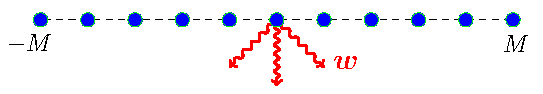
\includegraphics[width=1.0\columnwidth]{imm/sketch.eps}
    \caption{Sketch of a fermionic chain of size $L=2M+1$ subject to a
      localized particle loss at the central site, with strength
      controlled by the dissipation parameter $w$.  }
    \label{fig:sketch}
  \end{figure}
  
  
  As paradigmatic models we consider one-dimensional lattice models of
  non-interacting spinless fermionic gases, within hard-wall and
  harmonic traps, subject to dissipative perturbations that give rise to
  a particle loss localized at one of the sites of the lattice, such as
  the set up sketched in Fig.~\ref{fig:sketch}.  We model the
  dissipative particle-decay mechanism by Lindblad master equations
  governing the time evolution of the density
  matrix~\cite{Lindblad-76,GKS-76,BP-openquantumsystembook,RH-book,dr2021self}.  To
  investigate the effects of the localized particle-loss dissipation, we
  study the quantum dynamics arising from protocols starting from the
  ground state of the fermionic gas, then evolving under the effect of
  the particle-loss dissipation, for example localized at the center of
  the system.  This is analyzed in the large-$\ell$ limit for two
  different initial conditions: fixed number $N_0$ of initial particles
  and fixed ratio $N_0/\ell$, which corresponds to the {\em
    thermodynamic} limit of the initial fermionic gases at equilibrium,
  in both hard walls and harmonic traps.  The quantum evolution of the
  particle number and space-dependent density turns out to develop
  various dynamic scaling regimes, and nontrivial large-time behaviors
  when the dissipative mechanism acts at the center of the system.

  Some issues concerning the behavior of fermionic gases in the presence
  of localized dissipative interactions have been already discussed in
  Refs.~\cite{FCKD-19,LHFHCE-19,KMS-19,WSDK-20,FMKCD-20}, mainly
  for homogeneous systems neglecting boundary effects. Here we extend
  these studies by analyzing the interplay between time, size of the
  system, and number $N_0$ of initial particles. We analyze the various
  large-time and intermediate dynamic regimes, in both homogeneous
  particle systems within hard walls and inhomogeneous particle systems
  in harmonic traps. Substantially different and peculiar behaviors are
  observed in fermionic gases confined by hard walls and harmonic traps.
  
  
  The understanding of the interplay between the time dependence and the
  finite size of the system is essential to interpret results in various
  experimental contexts. For example this issue is fundamental for
  small-size quantum simulators operating on a limited amount of quantum
  objects, in the presence of controlled dissipation. We also mention
  experiments with cold atoms within a trap of finite size, when the
  many-body correlations become eventually sensitive to the trapping
  potential (local density approximations generally fail to describe
  quantum correlations, in particular when they are
  critical~\cite{CTV-13} and/or out-of-equilibrium~\cite{rossini2021coherent}).
  
  
  \subsection{Free lattice fermions  with localized dissipative defects}
  \label{modeldiss}
  
  \subsubsection{The Hamiltonian}
  \label{model}
  
  We consider one-dimensional $N$-particle Fermi gases defined on a
  chain with $L=2M+1$ sites, by the Hamiltonian
  \begin{equation}
    \hat H =
    - \kappa \sum _{x=-M}^{M-1} 
    (\hat c_{x}^\dagger \hat c_{x+1} +  \hat c_{x+1}^\dagger \hat c_{x})\,,
    \label{Hfree}
  \end{equation}
  where $\hat c_x$ is a fermion one-particle operator, and $\hat n_x =
  \hat c_x^\dagger c_x$ is the particle density operator.  We consider
  hard-wall (open) boundary conditions.  The site $x=0$ is the central
  site of the chain.  In the following we set $\hslash=1$ and $\kappa=1$
  without loss of generality.
  
  We also consider fermionic systems where the particles are trapped by
  an external potential, which can be taken into account by adding a
  corresponding term to the Hamiltonian (\ref{Hfree}), such as
  \begin{eqnarray}
    \hat H_t =
    - \sum _x 
    (\hat c_{x}^\dagger \hat c_{x+1} +  \hat c_{x+1}^\dagger \hat c_{x})
  +  \sum_x V(r) \, \hat n_x\,,\label{htrap}
    \end{eqnarray}
  where 
  \begin{eqnarray}
  \hat n_x =
  \hat c_x^\dagger c_x\,,\quad  V(r)= (r/L_t)^p\,, \quad r\equiv |x|\,,
     \label{potential}
  \end{eqnarray}
  $p$ is a positive number, $r$ is the distance from the center $x=0$ of
  the trap, and $L_t$ plays the role of trap size.~\footnote{$L_t$ plays
  the role of trap size~\cite{BDZ-08,RM-04,CV-10-2}, so that the {\em
    thermodynamic} limit is obtained in the large trap-size limit,
  $L_t\to \infty$, keeping the ratio between the particle number $N$ and
  the trap size $L_t$ constant, which can be equivalently obtained by
  adding a chemical-potential term in the Hamiltonian, such as the one
  reported in Eq.~(\ref{chemicalpot}).}  The trapping potential is
  effectively harmonic in most cold-atom experiments~\cite{BDZ-08},
  i.e., $p=2$.  In the limit $p\to\infty$ we recover the model
  (\ref{Hfree}) with hard-wall boundary conditions and $M=\lfloor L_t
  \rfloor$.  The size of systems described by the Hamiltonian $\hat H_t$
  with finite $p$ is supposed to be infinite. However for practical
  purposes it is sufficient to consider models within hard walls with $L
  \gg L_t$. Indeed the large-size convergence is generally fast for
  sufficiently large values of $p$, including $p=2$, due to the fact
  that the average particle density $\langle \hat{n}_x \rangle$ vanishes
  rapidly for $|x|\gg L_t$. The main features of the behavior of fermionic
  gases trapped by a inhomogeneous external power-law potentials have
  been much investigated, see e.g.
  Refs.~\cite{ACV-14,Nigro-17,CV-10,CV-10-2,Pollet-12}.
  
  In systems within both hard-wall and inhomogeneous traps, the particle
  number operator
  \begin{equation}
    \hat{N} = \sum_x \hat n_{x}\,
  \label{partnum}
    \end{equation}
  commutes with both Hamiltonians (\ref{Hfree}) and
  (\ref{htrap}). Therefore the particle number is conserved in both
  cases.  In the following we consider ground states for a number $N_0$
  of particles as starting point of dynamic protocols involving
  dissipative mechanisms.
  
  
  
  \subsubsection{Localized particle-decay dissipation}
  \label{locdiss}
  
  We model the dissipative mechanisms within the Lindblad
  framework~\cite{Lindblad-76,GKS-76}, where the evolution of the matrix
  density $\rho(t)$ of the system is described by he
  equation~\cite{BP-openquantumsystembook,RH-book}
  \eqref{eqlindblad}.
  We recall that the conditions leading to the Lindblad framework are
  typically satisfied in quantum optical
  implementations~\cite{BDS-2015-KeldyshOptical,dr2021self}.  The form of the operator
  ${\mathbb D}[\rho]$ depends on the nature of the dissipation arising
  from the interaction with the bath.  We consider a localized
  particle-decay dissipation acting at the site $z$, modeled by the
  Lindblad operator~\cite{HC-13, KMSFR-17, N-2019-uniquenesslindblad, NRV-2019-competingdissipativeandcoherent, WSDK-20,
    FMKCD-20, dr2021self,rossini2021coherent}
  \begin{eqnarray}
  \mathbb{D}[\rho] = w\,\biggr[
      \hat c_{z}\,\rho\,\hat c_{z}^\dagger - {1\over 2}\left( \rho\,
      \hat c_z^\dagger \hat c_{z} + \hat c_z^\dagger \hat c_{z} \rho \right)
      \biggr] \,, 
  \label{Lindop}
  \end{eqnarray}
  where $w$ is a parameter controlling the strength of the particle-loss
  dissipation.
  Note that reflection symmetry with respect to
    the center of the confined particle system is only preserved when
    the particle-loss dissipation is localized at the center. As we
    shall see, this will lead to peculiar behaviors with respect to the
    case of particle-loss dissipation localized at generic sites.
  
  
 
  \subsubsection{Dynamic protocol}
  \label{dynprot}
  
  To study fermionic gases under the effects of a localized
  particle-loss mechanism, we consider the following dynamic protocol,
  for systems within both hard-wall and harmonic traps, respectively of
  size $L=2M+1$ and $L_t$.
  
  \begin{itemize}
  
  \item[$\bullet$] The protocol starts at time $t=0$ from the ground
    state of the Hamiltonian (\ref{Hfree}) or (\ref{htrap}) with a
    number $N_0$ of particles. We recall that the ground state of $N_0$
    noninteracting fermionic particles is obtained by filling the lowest
    $N_0$ one-particle energy levels.
  
  \item[$\bullet$] The time evolution for $t>0$ is driven by the 
    Lindblad equation (\ref{eqlindblad}) for the density matrix
    $\rho(t)$, with particle-decay dissipation localized at a site $z$
    and controlled by the parameter $w$.
  
  \item[$\bullet$]
  The particle density and total particle number,  
  \begin{eqnarray}
  n_x(t) = {\rm Tr}[ \rho(t) \hat n_x ] \,,\qquad
  N(t) = {\rm Tr}\Bigr[ \rho(t) \hat N \Bigr] \,,
  \label{nxntdef}
  \end{eqnarray}
  are monitored during the out-of-equilibrium evolution for $t>0$, up to
  their large-time behaviors.
  
  \end{itemize}
  
  To compute the particle density $n_x(t)$ and particle number $N(t)$,
  we proceed as follows.  We introduce the correlation functions
  \begin{eqnarray}
    {\mathscr C}_{x,y}(t)= {\rm Tr}\Bigr[ \rho(t) \, \hat c_x^\dagger
      \hat c_y \Bigr] \,.
  \label{defct}
  \end{eqnarray}
  For homogeneous systems described by the Hamiltonian (\ref{Hfree}),
  the Lindblad equation (\ref{eqlindblad}) 
  implies
  \begin{eqnarray}
    {d\mathscr{C}_{x,y}\over dt} &=& i\,( \mathscr{C}_{x,y+1} -
     \mathscr{C}_{x-1,y} + \mathscr{C}_{x,y-1} - \mathscr{C}_{x+1,y} )
        \nonumber\\
      &&- \frac{w}{2} \ ( \delta _{z,y} + 
     \delta _{x, z} ) \, \mathscr{C}_{x,y} \,,
     \label{eqscxy}
  \end{eqnarray}
  where $\delta_{x,x}=1$ and $\delta_{x,y}=0$ for $x\neq y$.  Since we
  consider open (hard-wall) boundary conditions, ${\mathscr
    C}_{xy}(t)=0$ when the coordinates $x$ or $y$ refer to sites outside
  the space interval $[-M,M]$.  An analogous equation can be derived in
  the presence of an inhomogeneous external trapping potential,
  cf. Eq.~(\ref{htrap}).  We obtain
  \begin{eqnarray}
    &&  
    {d\mathscr{C}_{x,y}\over dt} = i\,( \mathscr{C}_{x,y+1} -
     \mathscr{C}_{x-1,y} + \mathscr{C}_{x,y-1} - \mathscr{C}_{x+1,y} )
     \nonumber\\
  &&\;\; + i {|x|^p - |y|^p\over L_t^p} \mathscr{C}_{x,y} 
  - \frac{w}{2} \ ( \delta _{z,y} + 
     \delta _{x, z} ) \, \mathscr{C}_{x,y} \,.
     \label{eqscxytrap}
  \end{eqnarray}
  Then, after numerically solving the above equations, we use the
  relations
  \begin{equation}
  n_x(t)=\mathscr{C}_{x,x}(t) \,,\qquad   N(t) = \sum _x n_x\,.
  \label{ntcxy}
  \end{equation}
  
  One can easily check that for both hard-wall and harmonic traps the
  derivative of the particle number is proportional to the average
  particle density $n_z$ at the site $z$ where the particle-decay
  dissipation is localized, i.e.
  \begin{equation}
    {d N(t)\over dt} = - w \, n_z(t) < 0\,.
  \label{ntnz}
  \end{equation}
  Therefore the particle number decays monotonically, since $n_z(t)\ge
  0$, and the particle loss stops if $n_z(t)= 0$ asymptotically.
  
  One may also consider the energy of the system, defined as
  \begin{eqnarray}
  E(t) = {\rm Tr}[\rho(t) \hat H] \,,
  \label{enedef}
  \end{eqnarray}
  for which the Lindblad equation implies
  \begin{eqnarray}
    {d E(t)\over dt} = {\rm Tr}\left[{d\rho(t)\over dt} \hat H\right]= w
    {\rm Tr}[{\mathbb D}[\rho] \,\hat H]\,.
    \label{detg}
  \end{eqnarray}
  For systems with particle-loss dissipation localized at the central
  site $x=0$, we obtain
  \begin{eqnarray}
    {d E(t)\over dt} =
    w \, {\rm Re}\,({\mathscr C}_{0,1}+{\mathscr C}_{-1,0}) =
    2 w \, {\rm Re}\,{\mathscr C}_{0,1}\,,
    \label{derene}
  \end{eqnarray}
  which holds for systems within hard walls and also inhomogeneous
  traps.
  
  \subsection{Fermi gases within hard walls}
  \label{hwbc}
  
  In this section we consider homogeneous Fermi chains, cf.
  Eq.~(\ref{Hfree}), and discuss the dynamic evolution under the
  particle-loss dissipation described by the Lindblad equation
  (\ref{eqlindblad}). We apply the Eq. \eqref{operatoreqlindblad} to the two-points correlation operator which for a non-interacting fermion system contains all its physical information. For this
  purpose, we numerically solve the differential equation (\ref{eqscxy})
  using the fourth-order Runge-Kutta method (with an accuracy of
  approximately $10^{-8}$ on the evolution of the particle number).
  
  We study the interplay between the time dependence, the number $N_0$
  of initial particles and the size $L=2M+1$ of the lattice.  For this
  purpose we consider two different situations: (i) the number $N_0$ of
  particles is kept fixed while increasing $M$; (ii) the number of
  particles is increases as $N_0\sim M$, so that the ratio $N_0/M$
  fixed, while increasing $M$. Note that the latter condition can be
  equivalently realized in the large-size limit by adding a chemical
  potential to the Hamiltonian (\ref{Hfree}), i.e.
  \begin{equation}
  \hat H_\mu = -(\mu+2) \sum _x \hat n_x \,.
  \label{chemicalpot}
  \end{equation}
  The value $\mu=\mu_{\rm vs}=-2$ corresponds to the vacuum-superfluid
  transition point~\cite{S99,ACV-14}, separating the phase
  where the lowest Hamiltonian eigenstate has $N=0$ particles from the
  one for $\mu>-2$ where the ground-state has $N\sim L$ fermions.
  
  In the following we first analyze the asymptotic large-time regime.
  Then we show that the time dependence of the particle number develops
  various asymptotic and intermediate regimes, which may differ in the
  cases we keep $N_0$ or $N_0/M$ fixed.
  
  
  \subsection{Asymptotic stationary states}
  \label{asysta}
  
  For generic locations of the particle-loss defects, the asymptotic
  stationary state turns out to be trivial, i.e. an empty state without
  particles. However in some cases, in particular when the defect is
  localized at the center of the chain, the quantum evolution of the
  system keeps a residual number of particles even in the large-time
  limit.
  
  This can be shown analytically, straightforwardly extending the
  analysis for non-interacting bosons reported in Ref.~\cite{KH-12}, to
  free fermions.  Since we are considering systems of size $L=2M+1$ with
  hard-wall boundary conditions, we introduce the fermionic operators
  \begin{eqnarray}
    \hat \eta_k = \sqrt{2\over L+1}
    \sum_{y=1}^{L} \sin\left({\pi k y \over L+1}\right)
    \hat c_y\,, \label{trafou}
  %  \hat c_y = \sqrt{2\over L+1} \sum_{k=1}^{L} \sin\left({\pi k y
  %  \over L+1}\right) \hat \eta_k \,,
  \end{eqnarray}
  where, to simplify the formulas, we have shifted the coordinates so
  that $y = x + M+1$ (therefore the site coordinates are $y=1,...,L$,
  and the center is located at $y=M+1$).  This allows us to write the
  Hamiltonian (\ref{Hfree}) as
  \begin{equation}
    \hat H = - 2 \sum_{k=1}^L \cos\left({\pi k\over L+1}\right) \hat n_k\,,
    \qquad   \hat n_k = \hat \eta_k^\dagger \hat \eta_k\,.
    \label{Hfreek}
    \end{equation}
  %Using the relations (\ref{trafou}), the Lindblad
  %operator (\ref{Lindop}) can be written as
  %\begin{eqnarray}
  %  \mathbb{D}[\rho] &=& {w\over L+1} \sum_{q,q'=1}^L \sin\left({\pi q z
  %    \over L+1}\right) \sin\left({\pi q' z \over L+1}\right)
  %  \nonumber\\ && \times \left( 2 \hat \eta_{q'} \rho \hat \eta_q^\dagger
  %  - \hat \eta_q^\dagger \hat \eta_{q'} \rho - \rho \hat \eta_q^\dagger \hat
  %  \eta_{q'} \right)\,.
  %    \label{drhokappa}
  %\end{eqnarray}
  The operator $\hat n_k$ commutes with the Hamiltonian, i.e. $[\hat
    H,\hat n_k] = 0$, and satisfies $\sum_k \hat n_k = \hat N = \sum_x
  \hat n_x$.  Its expectation value 
  \begin{equation}
  n_k(t) = {\rm Tr}[\rho(t)\, \hat n_k]\,
  \label{nkope}
  \end{equation}
  counts the number of particles associated with the mode $k$.  The
  initial equilibrium ground state with $N_0$ fermionic particles is
  constructed by filling the first $N_0$ one-particle energy levels,
  thus at $t=0$ we have $n_k=1$ for $k\le N_0\le L$, and zero
  otherwise. The modes with odd (even) $k$ are even (odd) under
  inversion with respect to the center $y=M+1$ of the chain.  The time
  evolution of $n_k$ is determined by the Lindblad equation for the
  density matrix.  Considering a particle-decay dissipation located at a
  generic site $z$, straightforward calculations lead to the equation
  \begin{eqnarray}
    {d n_k\over dt} &=&
  %  - {w\over M+1} \sum_{q,q'=1}^M \sin\left({\pi q z
  %  \over M+1}\right) \sin\left({\pi q' z \over M+1}\right)
  %\nonumber\\ &&\times (\delta_{kq} + \delta_{kq'}) {\rm Tr}[\rho(t) \,
  %  \hat \eta_q^\dagger \hat \eta_{q'}]\,
  %\nonbumber \\
  - {w\over L+1} \sin\left({\pi k z \over L+1}\right)
  \label{ddtnk} \\
  &\times& \sum_{q=1}^L \sin\left({\pi q z\over L+1}\right)
  {\rm Tr}[\rho(t) \,
  (\hat \eta_q^\dagger \hat \eta_{k} + \eta_k^\dagger \hat \eta_{q})]\,,
  \nonumber
  \end{eqnarray}
  where, due to the fact that $[\hat H,\hat n_k]=0$, the only
  contribution to the time derivative of $n_k$ comes from the
  dissipative term.  We note that the r.h.s. of Eq.~(\ref{ddtnk})
  vanishes when
  \begin{equation}
  k z = j (L+1)\,, \quad j=1,2,...,
  \label{kz}
  \end{equation}
  thus implying the conservation of the corresponding particle number
  $n_k$ even in the presence of localized particle-decay dissipation.
  
  
  \begin{figure}[!htb]
\centering
    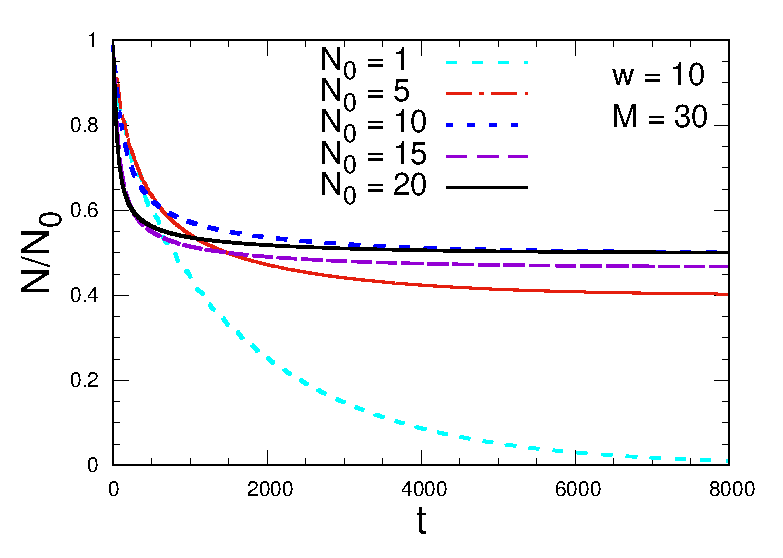
\includegraphics[width=0.65\columnwidth]{imm/Now10.eps}
    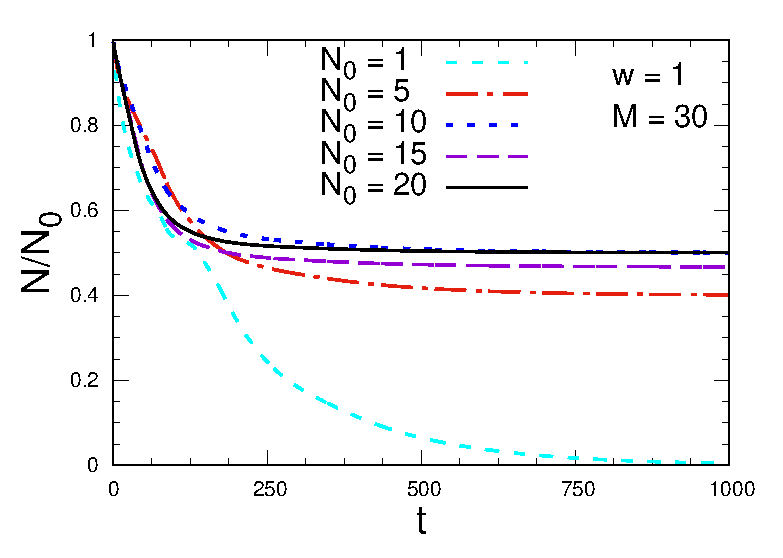
\includegraphics[width=0.65\columnwidth]{imm/No.eps}
    \caption{Behavior of the ratio $N(t)/N_0$ for the central-site
      particle-loss dissipation in systems of size $L=61$ ($M=30$)
      within hard walls, various initial particle number $N_0$, and
      dissipation localized at the center of the system, with $w=1$
      (bottom) and $w=10$ (top).  In both cases asymptotic stationary
      limit turns out to converge to $N/N_0=1/2$ for even $N_0$, and
      $N/N_0=(N_0-1)/(2N_0)$ for odd $N_0$.  Note that approach to the
      asymptotic value is slower for $w=10$ than $w=1$.}
    \label{ndiffn0}
  \end{figure}
  
  
  
  If we consider a central-site dissipation, thus $z=M+1=(L+1)/2$ [we
    recall that we are using shifted coordinates with respect to
    Eq.~(\ref{Hfree})], then the condition (\ref{kz}) reduces to $k=2j$,
  thus implying that $n_k$ remains unchanged for all even $k$ (whose
  odd-parity modes vanish at the central dissipative site), while it
  gets suppressed for odd $k$. Therefore, Eq.~(\ref{ddtnk}) implies that
  half of the fermions survives centrally localized decay
  dissipation. More precisely the stationary states are characterized by
  a residual particle number $N_{\rm asy} = N_0/2$ for even $N_0$, and
  $N_{\rm asy} = (N_0-1)/2$ for odd $N_0$.
  
  Note that the particle loss localized at the center, preserving the
  parity symmetry with respect to the center of the chain, is the
  optimal one to keep a fraction of fermionic particles at large time.
  For example, in the case of a dissipation at the boundaries, i.e.,
  when $z=1$ or $z=M$ in Eq.~(\ref{ddtnk}), no particles survive because
  all $k$-modes are involved by the Lindblad operator, leading to the
  complete suppression of the particles filling the initial ground
  state.
  
  \begin{figure}[!htb]
\centering
    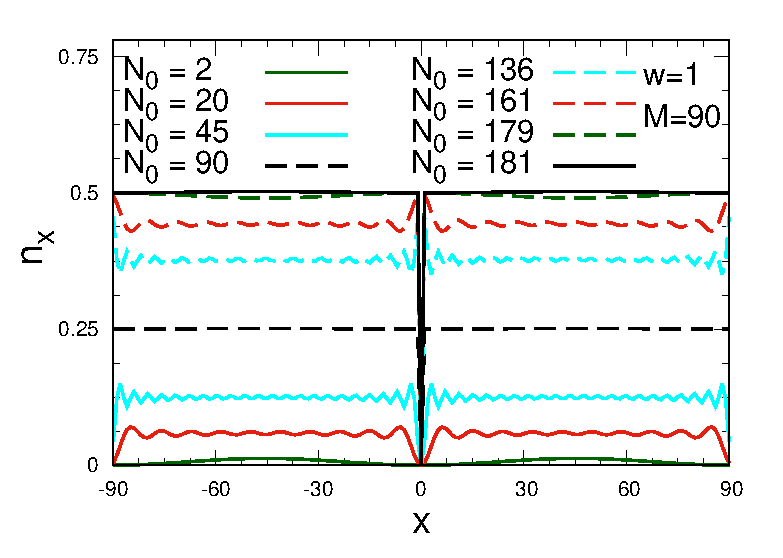
\includegraphics[width=0.65\columnwidth]{imm/nxhwall.eps}
    \caption{Data for the quantum evolution of the fermionic gas within
      hard walls, size $L=2M+1$ with $M=90$, initial particle number
      $N_0=10$, dissipation localized at the center of the chain with
      $w=1$. We show the particle density $n_x(t)$ at the sites $x=0$
      and $x=10$ (top), and the ratio $N(t)/N_0$ (bottom).  They
      approach asymptotic stationary limits (at least within the
      numerical precision, which is very accurate).}
    \label{nxdiffn0time}
  \end{figure}

  
  \begin{figure}[!htb]
\centering
    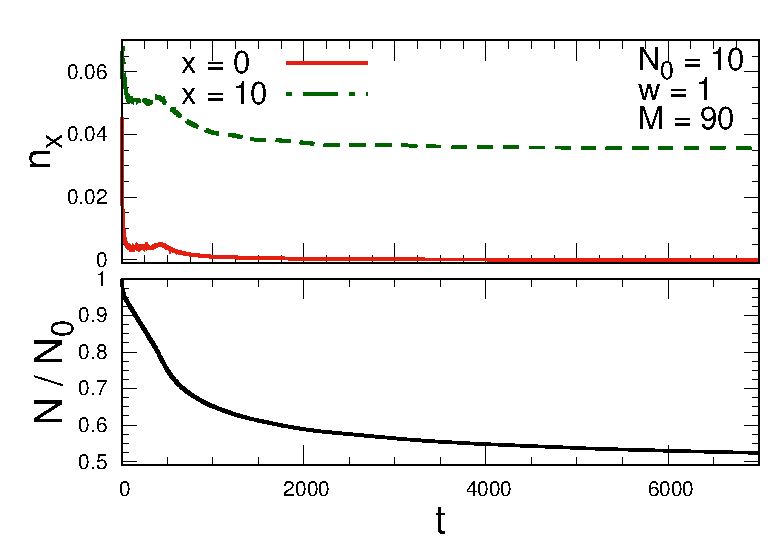
\includegraphics[width=0.65\columnwidth]{imm/nxNo.eps}
    \caption{Asymptotic stationary limit of the particle density $n_x$
      for systems of size $L=181$ ($M=90$) within hard-wall boundary
      conditions, in the presence of a central-site dissipation with
      $w=1$, and for various $N_0$. In all cases the particle density
      vanishes for $x=0$, and it is almost flat elsewhere, apart from
      small spatial oscillations, which appear similar to the
        Friedel oscillations characterizing the behavior of closed
        particle systems}.
    \label{nxdiffn0}
  \end{figure}
  
  
  The above analytical results are confirmed by the numerical results
  for the central particle-loss dissipation, see for example
  Fig.~\ref{ndiffn0} where we show the time dependence of the ratio
  $N(t)/N_0$ for various values of $N_0$ and $w$, and in particular the
  approach to its nonzero asymptotic limit. Also the space dependence of
  the particle density $n_x$ turns out to become stable asymptotically,
  approaching a stationary configuration, as shown in
  Fig.~\ref{nxdiffn0time}.  In Fig.~\ref{nxdiffn0} we show some results
  for the spatial dependence of the average particle density $n_x$ of
  the asymptotic stationary states. We note that $n_x$ is quite flat
  except at $x=0$ where the dissipative mechanism acts, and at the
  boundaries of the chain (essentially due to the hard-wall boundary
  conditions). The almost flat region shows some spatial oscillations,
  which appear suppressed when $N_0\approx M$ and $N_0\approx 2M$.
  
  
  \subsection{Approach to the asymptotic states}
  \label{asyappro}
  
  
  \subsubsection{Large-size behavior of the Liouvillian gap}
  \label{liogap}
  
  
  
  The approach to the stationary state is controlled by the Liouvillian
  gap $\Delta_{\cal L}$ of the generator ${\cal L}$ of the Lindblad
  equation~\cite{BP-openquantumsystembook,RH-book,Z-2015-relaxtimes,MBBC-18,KS-2020-boundarydephasing},
  \begin{equation}
  \Delta_{\cal L} = - {\rm Max}_{i>0} \, {\rm Re}\,(\Lambda_i)\,,
  \label{deltadeb}
  \end{equation}
  where $\Lambda_i$ are the eigenvalues of ${\cal L}$ (we recall that
  the largest eigenvalue is $\Lambda_0=0$ and ${\rm Re} \,\Lambda_i<0$
  for any $i>0$).  The Liouvillian gap for homogeneous spin chains and
  fermionic wires with localized dissipative mechanisms, such as that
  described by Eq.~(\ref{Lindop}), shows generally the asymptotic
  finite-size
  behavior~\cite{PP-08,P-2008-thirdquantization,Z-2015-relaxtimes,KS-2020-boundarydephasing,TV-2021-dissipativeboundaries}
  \begin{equation}
  \Delta_{\cal L}(w,L)\approx D_{\cal L}(w) \,L^{-3}\,.  
  \label{deltaL}
  \end{equation}
  We expect that this asymptotic large-$L$ behavior holds independently
  of the location of the particle-decay dissipation, and it does not
  depend on the initial conditions, thus on $N_0$.  The scaling equation
  (\ref{deltaL}) implies that the approach to the asymptotic behavior
  becomes slower and slower with increasing the size $L$ of the lattice
  at fixed $w$.
  
  \begin{figure}[!htb]
\centering
    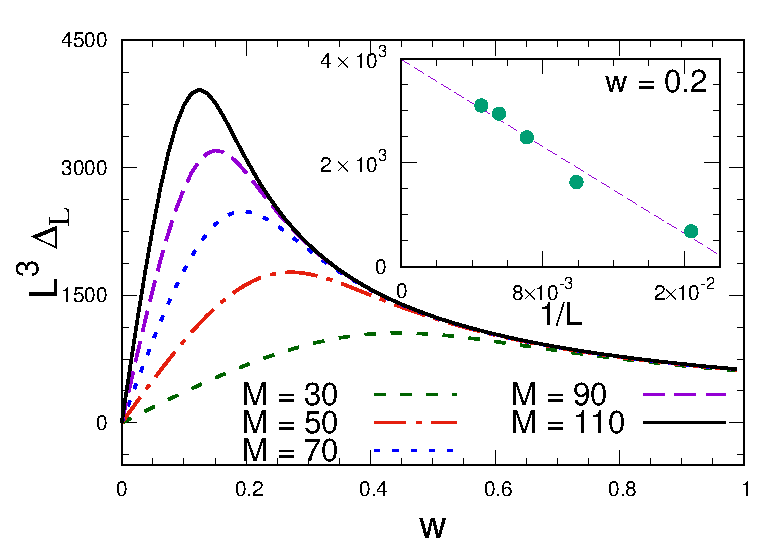
\includegraphics[width=0.65\columnwidth]{imm/DeltawNoL3.eps}
    \caption{The Liouvillian gap $\Delta_{\cal L}$ for particle-decay
      dissipation localized at the center of the chain, for various
      system size $L=2M+1$. The curves appear to converge with
      increasing $M$; this is clearly shown at least for $w\gtrsim 0.2$,
      as also shown by the large-$L$ convergence at a fixed value
      $w=0.2$ [suggesting that the corrections to the asymptotic scaling
      behavior (\ref{deltaL}) are approximately $O(L^{-1})$].  Like the
      case of dissipation at the boundaries, we believe that the
      convergence extends to any $w>0$, but, unlike dissipation at the
      boundaries, it is nonuniform when decreasing $w$ toward zero, see
      text.} 
    \label{liogaps}
  \end{figure}
  
  
  \begin{figure}[!htb]
\centering
    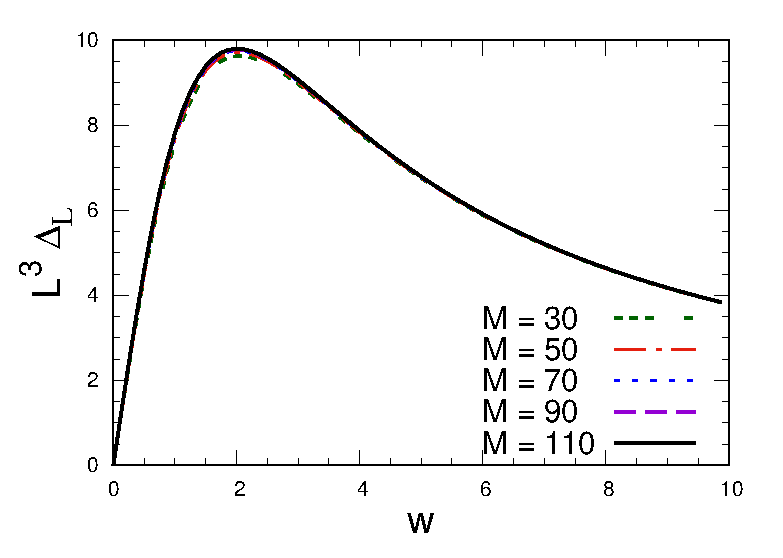
\includegraphics[width=0.65\columnwidth]{imm/deltaextr.eps}
    \caption{Scaling behavior of the Liouvillian gap $\Delta_{\cal L}$
      for particle-decay dissipation localized at one of the boundaries
      of the chain.}
        \label{liogapsb}
  \end{figure}
  
  
  
  
  \begin{figure}[!htb]
\centering
      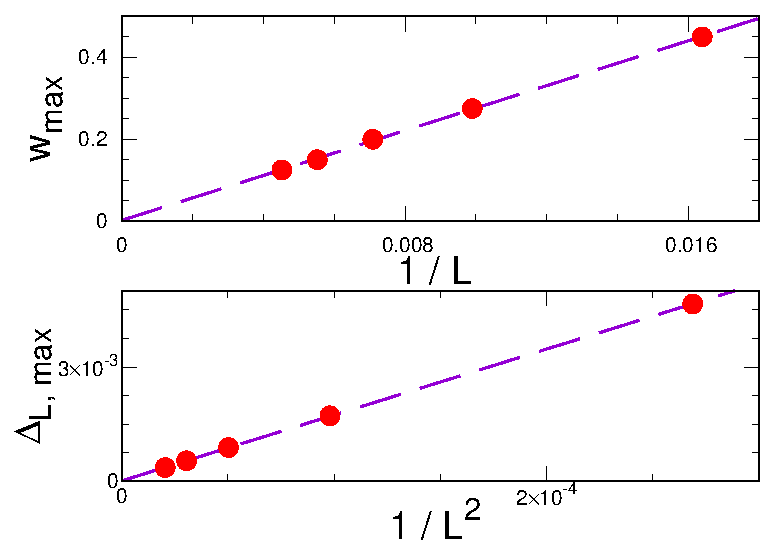
\includegraphics[width=0.65\columnwidth]{imm/wDmax1.eps}
    \caption{Some details of the behavior of the Liouvillian gap
      $\Delta_{\cal L}$ for dissipation localized at the center of the
      lattice. We show the location $w_{\rm max}$ of the maximum of the
      Liouvillian gap (top), showing that $w_{\rm max}\sim L^{-1}$, and
      value of $\Delta_{\cal L}$ at the maximum (bottom), showing that
      $\Delta_{\cal L}(w_{\rm max})\sim L^{-2}$.}
    \label{gapcenterdetails}
  \end{figure}
  
  
  \begin{figure}[!htb]
\centering
    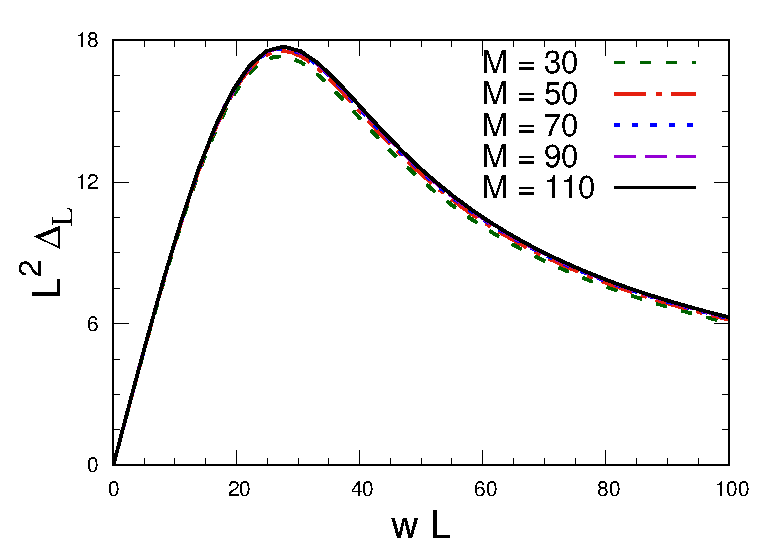
\includegraphics[width=0.65\columnwidth]{imm/DeltawLNo.eps}
    \caption{Plots of $L^2 \Delta_{\cal L}$ versus $wL$ for systems
      within hard walls and with central particle-loss dissipation, for
      various $L=2M+1$.  They support the scaling equation
      (\ref{deltaLcenter}).}
        \label{gapcenter2}
  \end{figure}
  
  The asymptotic behavior (\ref{deltaL}) is confirmed by numerical
  analyses of the Liouvillian gap using the method outlined in
  Ref.~\cite{PP-08}, see App.~\ref{appa}. Some numerical results are
  shown by Figs.~\ref{liogaps} and \ref{liogapsb}, for particle-decay
  dissipation localized at the center and at the boundary of the chain,
  respectively.
  
  In both cases, $\Delta_{\cal L}$ appears nonmonotonic, increasing for
  small values of $w$ and decreasing for sufficiently large dissipation
  strength $w$, for any $L$.  The approach to the asymptotic behavior
  becomes slower and slower with increasing $w$ for large $w$. In
  particular, $\Delta_{\cal L}(w,L)$ shows the large-$w$ behavior $L^3
  \Delta_{\cal L}(w)\approx D_{\cal L}(w)\sim w^{-1}$. This explains the
  results shown in Fig.~\ref{ndiffn0}, where the approach to the
  asymptotic value of the particle number for $w=10$ turns out to be
  slower than that for $w=1$.  The suppression in the limit of
    strong dissipation, for large $w$, may be interpreted as a
    quantum-Zeno-like phenomenon~\cite{MS-1977-quantumzeno,FP-08}, where a strong
    dissipation somehow slows down the dynamics, see
    e.g. Refs.~\cite{TNDTT-17,DMSD-20} for the appearence of similar
    quantum Zeno regimes.
  
  As shown by Figs.~\ref{liogaps} and \ref{liogapsb}, the Liouvillian
  gap at fixed $L$ has a maximum at an intermediate value of
  $w$. The corresponding values $w_{\rm max}$ and $L^3 \Delta_{\cal
      L}(w_{\rm max})$ appears to rapidly converge to the large-$L$
    limit in the case of dissipations localized at the boundaries, but
    they show an apparent size dependence in the case of dissipation
    localized at the center. Indeed the approach to the asymptotic
    $L^{-3}$ behavior (\ref{deltaL}) appears significantly slower in the
    case of dissipation localized at the center, in particular for small
    $w$, which suggests a nonuniform convergence for $w\to 0$.  The
    curves for different lattice sizes appear to clearly converge for
    $w\gtrsim 0.2$, as also shown by the inset of Fig.~\ref{liogaps}. We
    conjecture that, like the case of dissipation at the boundaries, the
    convergence in the large-size limit extends to any $w>0$, but it is
    nonuniform when decreasing $w$ toward zero, unlike dissipation at
    the boundaries.  This is demonstrated by the plots reported in
  Figs.~\ref{gapcenterdetails}, which show that the location of the
  maximum value of the Liouvillian gap for central dissipation moves
  toward $w=0$, with $w_{\rm max}\sim L^{-1}$, and its maximum value
  decreases as $\Delta_{\cal L}(w_{\rm max})\sim w_{\rm max}^2\sim
  L^{-2}$, instead of the general asymptotic $L^{-3}$ behavior for $w>0$
  fixed. Actually, they suggest that the Liovillian gap for central
  dissipation shows also the asymptotic scaling behavior
  \begin{equation}    
  \Delta_{\cal L}(w,L)\approx {\cal D}_{\cal L}(wL) \,L^{-2}\,,
  \label{deltaLcenter}
  \end{equation}
  obtained in the large-$L$ limit keeping $wL$ constant.  This scaling
  behavior is demonstrated by the plot reported in
  Fig.~\ref{gapcenter2}.  Therefore the function $D_{\cal L}(w)$
  entering the asymptotic $L^{-3}$ behavior (\ref{deltaL}) must be
  singular for $w\to 0$ in the case of central-site dissipation,
  diverging as $w^{-1}$.
  
  Note that the above considerations on the behavior of the Liouvillian
  gap apply to generic values of $w$, and,  of course, they do not depend
  on the initial number $N_0$ of particles.  In the following we will
  mainly present results for the value $w=1$ of the dissipation
  parameter, whose dynamic scenarios are shared with those arising from
  generic finite values of $w$.
  
  \subsubsection{Large-time behavior of the particle number}
  \label{lasypgap}
  
  On the basis of the large-size behavior of the Liouvillian gap, we
  expect that the time scale $t_a$ of the approach to the stationary
  state is given as
  \begin{equation}
  t_a \sim \Delta_{\cal L}^{-1}\sim L^3\,,
  \label{timescaleasy}
  \end{equation}
  at fixed $w>0$. This time scale must characterize the approach to the
  stationary limits of the particle number and density.  This is
  confirmed by the numerical computations, see for example
  Fig.~\ref{rntn010} where we report results for the ratio
  \begin{equation}
    R_N(t)\equiv {N(t)-N_{\rm asy}\over N_0-N_{\rm asy}}\,,
      \label{defqu}
  \end{equation}
  for protocols starting from a fixed number $N_0$ of particles.  They
  show the asymptotic large-$L$ scaling behavior
  \begin{eqnarray}
    R_N(t,w,L) \approx A(t/L^3,w)\,,\label{scalbehasy}
  \end{eqnarray}
  which also implies
  \begin{eqnarray}
  {d R_N(t,w,L)\over dt} &\approx& L^{-3} B(t/L^3,w)\,.  \nonumber
  \end{eqnarray}
  Analogous results are obtained for the case we start from a fixed
  ratio $N_0/M$, as shown in Fig.~\ref{dntln0lasy} for $N_0/M=1/2$,
  where we plot $N(t)-N_{\rm asy}$ versus $t/L^3$ and the curves appear
  to collapse in the large-$M$ limit. Note that when $N_0/M$ is kept
  fixed, the quantity $R_N$ defined in Eq.~(\ref{defqu}) is not
  appropriate, because it is always suppressed in the large-time limit,
  due to the denominator that behaves as $N_0-N_{\rm asy}\sim L$.
  
  
  \begin{figure}[!htb]
\centering
    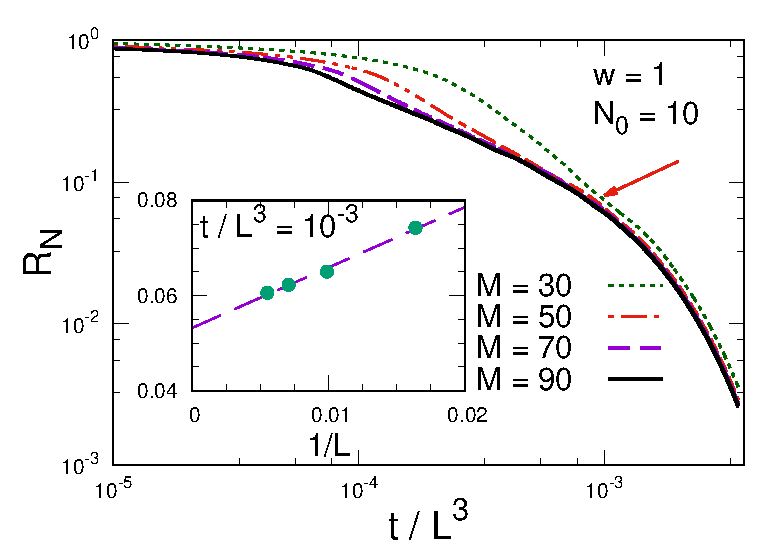
\includegraphics[width=0.65\columnwidth]{imm/NL3.eps}
    \caption{The time dependence of the ratio $R_N$ versus $t/L^3$
      ($L=2M+1$), for homogenous systems within hard walls with $N_0=10$
      and central particle-loss dissipation with $w=1$.  The data for
      various sizes $M$ show clearly the convergence toward a dynamic
      scaling curve, approximately as $1/L$ as shown by the inset for a
      particular value of the ratio $t/L^3$ (the one indicated by the
      arrow in the main figure).}
    \label{rntn010}
  \end{figure}
  
  
  \begin{figure}[!htb]
\centering
    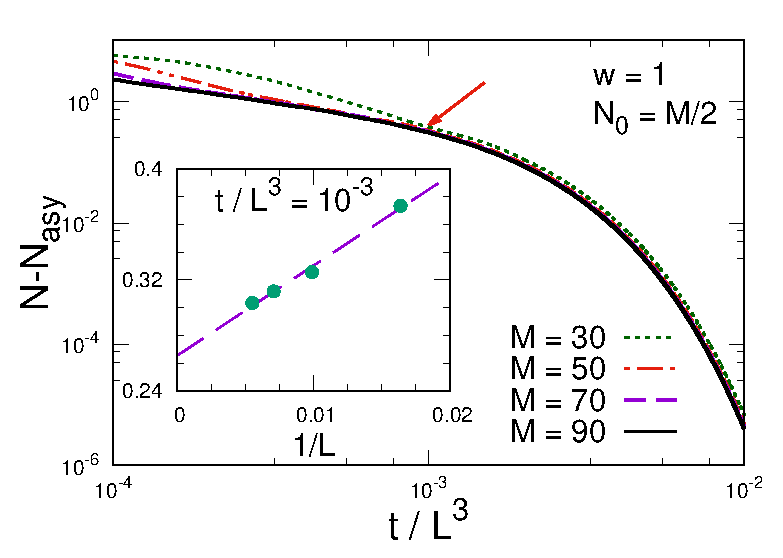
\includegraphics[width=0.65\columnwidth]{imm/dNLL3.eps}
    \caption{The difference $N(t) - N_{\rm asy}$ vs $t/L^3$, for systems
      within hard walls with $N_0/M=1/2$, and central dissipation with
      $w=1$.  Again we observe the asymptotic convergence toward a
      dynamic scaling curve, as shown by the inset for a particular
      value of $t/L^3$ (indicated by the arrow in the main figure).}
    \label{dntln0lasy}
  \end{figure}
  
  As we will show below, this is not the end of the story, indeed
  further peculiar intermediate scaling behaviors emerge, differing
  between the cases $N_0$ and $N_0/M$ fixed.
  
  
  
  
  \subsection{Intermediate scaling behaviors keeping $N_0$ fixed}
  \label{N0fixed}
  
  \begin{figure}[!htb]
\centering
    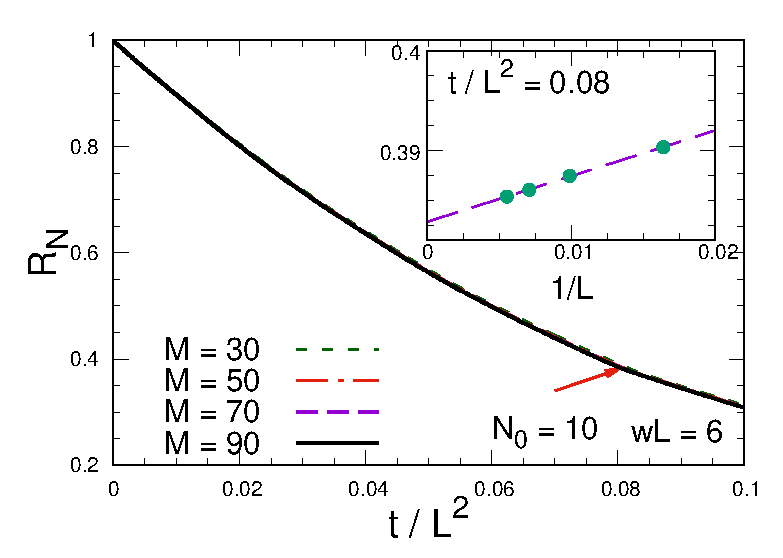
\includegraphics[width=0.65\columnwidth]{imm/NwL2.eps}
    \caption{The ratio $R_N$ versus $t/L^2$ for systems within hard
      walls with $N_0=10$, central dissipation with $wL=6$, for various
      lattice sizes $L=2M+1$.  The data appear to converge toward a
      scaling curve in the large-$L$ limit, as demonstrated by the data
      reported in the inset for a particular value of the ratio
      $t/L^2$.}
    \label{rntn010ir}
  \end{figure}
  
  We now look for intermediate regimes of the time evolution, somehow
  associated with the time scales of the Hamiltonian (\ref{Hfree})
  driving the unitary dynamics, and therefore to its gap $\Delta_H$,
  i.e. the energy difference between the first excited state and the
  ground state. When keeping the particle number $N_0$ fixed, $\Delta_H$
  behaves asymptotically as $\Delta_H \sim L^{-2}$, corresponding to the
  dynamic exponent $z=2$ of the vacuum-superfluid
  transition~\cite{S99}.
  
  We want to check whether the
    out-of-equilibrium dynamics develops an intermediate regimes somehow
    controlled by the Hamiltonian driving of the Lindblad equation,
    whose intrinsic time scale is related to its gap, i.e. $t \sim
    \Delta_H^{-1}\sim L^2$, which is much smaller than the time scale
    $t\sim L^3$ characterizing the approach to the stationary large-time
    limit (of course, for sufficiently large $L$, and in particular in
    the large-$L$ limit). As we shall see, a closer look at the time
    evolution provides a clear evidence of such intermediate regime, which 
     also requires a rescaling of the dissipation strength.
  
  
  In Fig.~\ref{rntn010ir} we show some results for the time dependence
  of the particle number in the case of systems with central-site
  dissipation starting from a fixed number of particles. We observe that
  the above-mentioned intermediate regime exists, and extends to any
  $t\sim L^2$, if we perform an appropriate rescaling of the dissipation
  parameter $w$, decreasing $w$ as $w\sim L^{-1}$. Indeed the numerical
  results clearly support the large-$L$ scaling behavior
  \begin{eqnarray}
   R_N(t,w,L) \approx U(t/L^2,wL)\,,   \label{scalbehwl}
  %%  L^2 {d R_N(t,w,N_0,L)\over dt} &\approx& W(t/L^2,wL)\,,\nonumber
  \end{eqnarray}
  which is obtained by increasing $L$ keeping the ratio $t/L^2$ and the
  product $wL$ fixed.  Note that this intermediate scaling behavior is
  expected to hold even for large values of the ratio $t/L^2$, because
  it is also compatible with the alternative scaling behavior
  (\ref{deltaLcenter}) of the Liouvillian gap.
  
  
  
  
  
  
  \subsection{Intermediate dynamic behavior keeping $N_0/M$ fixed}
  \label{N0oLfixed}
  
  \begin{figure}[!htb]
\centering
    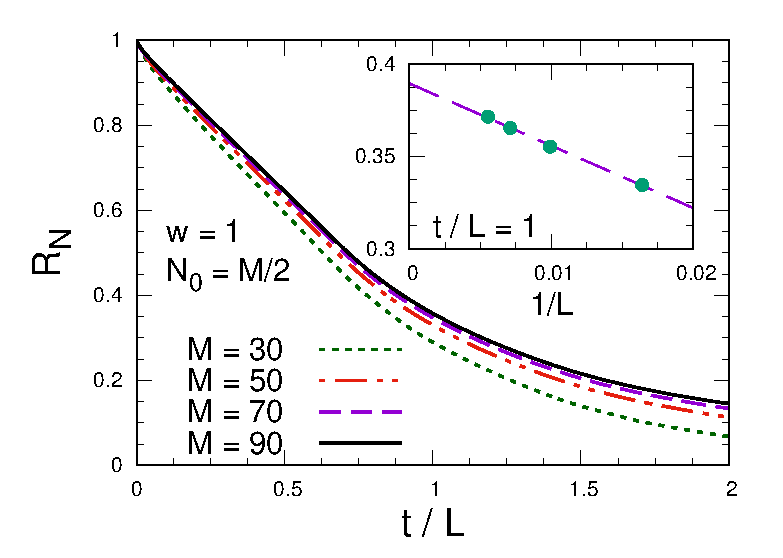
\includegraphics[width=0.65\columnwidth]{imm/NLL1.eps}
    \caption{Behavior of the ratio $R_N$ versus $t/L$, for systems
      within hard walls with $N_0/M=1/2$, and central dissipation with
      $w=1$. The inset shows the $1/L$ approach to the large-$L$
      asymptotic behavior.}
    \label{rntn0lvstol}
  \end{figure}
  
  We now consider the large-$L$ behavior in the case we keep the ratio
  $N_0/M$ fixed when increasing $L=2M+1$. This corresponds to the
  superfluid phase, i.e. when the chemical potential $\mu$ is larger
  than that at the vacuum-superfluid transition, $\mu>-2$. Within the
  superfluid phase, the gap $\Delta_S$ of isolated free Fermi gases
  behaves as~\cite{S99} $\Delta_S \sim L^{-1}$.
  
  Again we want to check whether the out-of-equilibrium dynamics in
    this condition develops an intermediate regime controlled by the
    part of the Lindblad equation driving the unitary dynamics
    introduces a time scale $t\sim \Delta_S^{-1}\sim L$ (again, much
    smaller than the time scale $t\sim L^3$ characterizing the approach
    to the stationary large-time limit). Like the case at fixed $N_0$,
    we show that such an intermediate regime exists.
  
  The existence of a corresponding intermediate regime of the dynamics
  is demonstrated by the results shown in Fig.~\ref{rntn0lvstol},
  leading to the intermediate scaling ansatz
  \begin{eqnarray}
   R_N(t,w,L) \approx W(t/L,w)\,,   \label{scalbehnol}
  %%  L {d R_N(t,w,L)\over dt} &\approx& W(t/L,w)\,,\nonumber
  \end{eqnarray}
  obtained keeping $t/L$ fixed in the large-$L$ limit.  
  
  We finally report the existence of a further early-time regime when we
  start from the ground state for $N_0\propto M$, as already noted in
  Ref.~\cite{FMKCD-20}. Indeed, for sufficiently small time
  \begin{equation}
    {d N(t,w,L)\over dt} \approx  f(t,w)\,,
    \label{vereg}
    \end{equation}
  without showing any asymptotic size dependence.  This is shown by the
  curves reported in Fig.~\ref{rntln0lvst}.  The behavior (\ref{vereg})
  is observed in the large-size limit, and can be considered as the {\em
    thermodynamic} limit of the quantum evolution, when the time is
  sufficiently small that the dynamics does not yet detect the effects
  of the boundaries.  Indeed deviations are observed for $t\propto M$,
  thus later and later for larger and larger systems. At the end of this
  early-time regime, the intermediate regime (\ref{scalbehnol}) begins.
  
  
  
  \begin{figure}[!htb]
\centering
  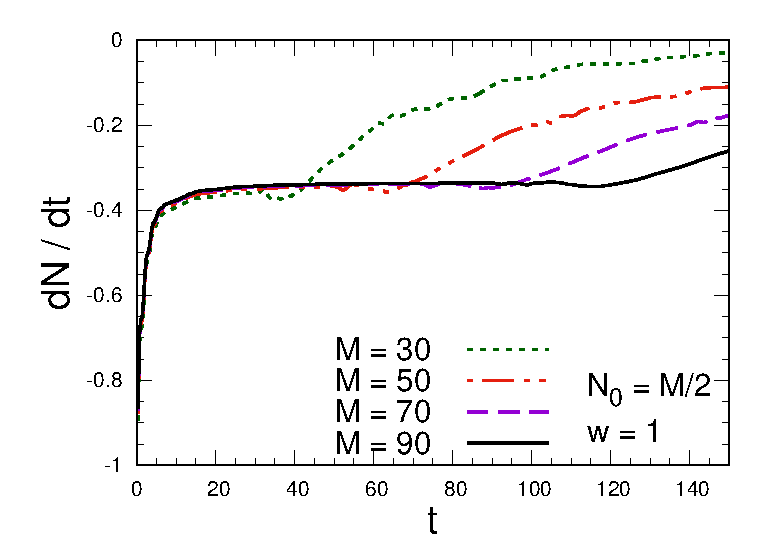
\includegraphics[width=0.65\columnwidth]{imm/dNLL0.eps}
  \caption{The time dependence of the derivative of the particle number,
    for systems within hard walls with central-site dissipation with
    $w=1$, starting from ground states with $N_0/M=1/2$ fixed.  }
    \label{rntln0lvst}
  \end{figure}
  
  
  
  \section{Fermionic gases within harmonic traps}
  \label{hartra}
  
  
  We now present results for lattice fermionic systems within traps
  arising from inhomogeneous external potentials, such as those in
  Eq.~(\ref{potential}), in the presence of a particle-decay dissipation
  at the center of the trap, as described by the Lindblad equations
  (\ref{eqlindblad}) and (\ref{Lindop}). As already mentioned in
    the introductive section, effective harmonic trapping mechanisms are
    quite common in cold-atom experiments~\cite{BDZ-08}. Therefore their
    analysis is also relevant from a phenomonological point of view.
  
  We study the time evolution in the limit of large trap size $L_t$, in
  the case we keep the initial particle number $N_0$ fixed, and when we
  keep the ratio $N_0/L_t$ constant (equivalent to addiing a chemical
  potential). We consider harmonic traps, thus $p=2$ in
  Eq.~(\ref{potential}). The results are obtained for sufficiently large
  systems $L$ at fixed $L_t$, so that a further increases of $L$ does
  not change the results at fixed $L_t$, and therefore they can be
  considered as results for infinite-size systems with a large accuracy,
  within the accuracy of the numerical calculations, better than
  $10^{-8}$.
  
  
  \subsection{Large-time behavior}
  \label{asytrap}
  
  \begin{figure}[!htb]
\centering
    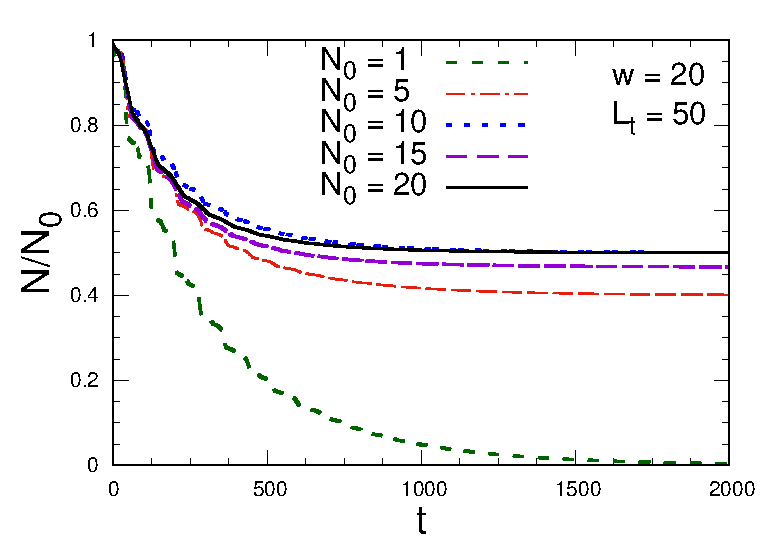
\includegraphics[width=0.65\columnwidth]{imm/trapNow20.eps}
  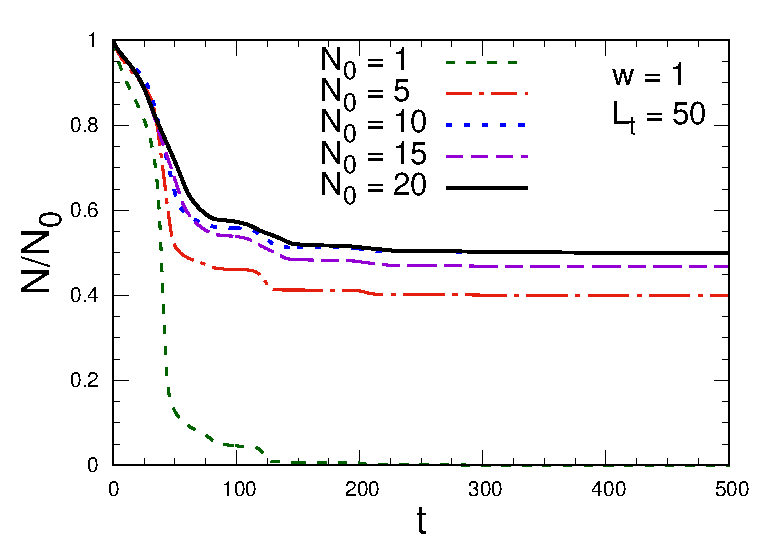
\includegraphics[width=0.65\columnwidth]{imm/trapNo.eps}
  \caption{The time dependence of the ratio $N/N_0$ for the central-site
    particle-loss dissipation $w=1$ (bottom) and $w=20$ (top) in systems
    within harmonic traps, various $N_0$, and $L_t=50$ (in the large-$L$
    limit to make the finite-size effects negligible).  The asymptotic
    stationary limit turns out to converge to $N/N_0=1/2$ for even
    $N_0$, and $N/N_0=(N_0-1)/(2N_0)$ for odd $N_0$. Similarly to the
    case of systems within hard walls, see Fig.~\ref{ndiffn0}, the
    approach to the asymptotic value turns out to be slower for $w=20$
    than $w=1$.}
  \label{traptdep}
  \end{figure}
  
  
  To begin with, we discuss the asymptotic stationary states.  In
  Fig.~\ref{traptdep} we show the time dependence, and asymptotic
  behavior, of the ratio $N(t)/N_0$ for various values of the initial
  number of particles. Again, similarly to the case of homogeneous
  systems within hard walls and particle-decay dissipation at the center
  of the chain, we find that the large-time states keep a half of the
  initial particles.  Analogously to the hard-wall case, this can be
  related to the fact that the one-particle Hamiltonian is invariant
  under reflections with respect to the center, thus the one-particle
  states must have definite parity. This can be easily seen in the
  continuum limit, see e.g. Ref.~\cite{ACV-14}, where the one-particle
  Hamiltonian eigenfunctions can be written in terms of Hermite
  polynomials, and have definite parity.  Since the one-particle states
  with negative parity vanishes at the center of the trap, the
  corresponding modes in the ground state of the fermionic system are
  not affected by the particle-decay dissipation at the center of the
  trap. Then, recalling that the ground state is obtained by filling the
  first $N_0$ one-particle levels, a selection mechanism analogous to
  that identified in the case of homogeneous systems applies, see
  Sec.~\ref{asysta}, therefore half of them are odd [more precisely
    $N_0/2$ for even $N_0$ and $(N_0-1)/2$ for odd $N_0$], we expect
  again that half particles survive the central particle loss.
  
  \begin{figure}[!htb]
\centering
  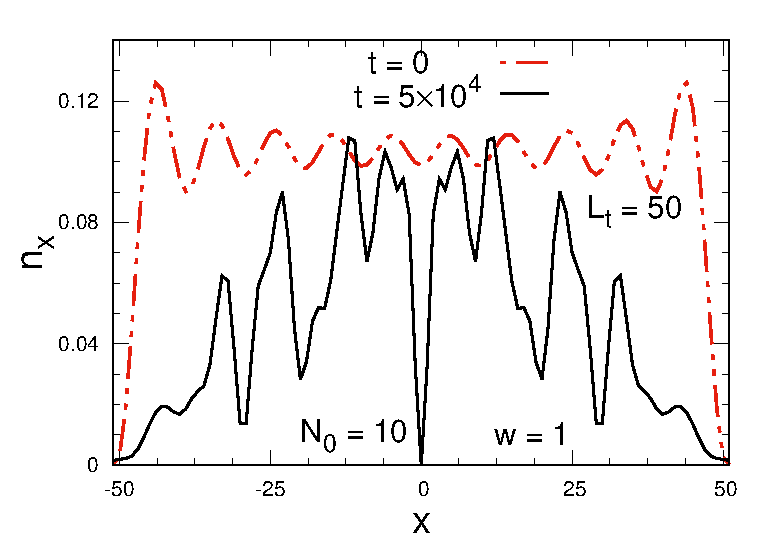
\includegraphics[width=0.65\columnwidth]{imm/trapnxLt50.eps}
  \caption{The particle density $n_x$ for systems within a harmonic trap
    with initial particle number $N_0=10$, at $t=0$ and after some time
    $t$, for a central dissipation with $w=1$, fixed trap size $L_t=50$,
    and for a sufficiently large size of the system, $L=221$, to make
    finite-size effects negligible (numerically checked by verifying the
    dependence on $L$).}
  \label{trapnxt}
  \end{figure}
  
  In Fig.~\ref{trapnxt} we show the particle density at $t=0$ and at
  large time when the central particle density has already stably
  vanished. However, the spatial dependence of the particle density does
  not appear static in the large-time regime where the particle number
  stops decreasing. Indeed, as shown in Fig.~\ref{trapnxto}, the time
  dependence of the particle density at sites $x\neq 0$ is characterized
  by time oscillations that apparently continue indefinitely, persisting
  even in the large-$L_t$ limit.  We also note that in this large-time
  regime the quantum evolution of the particle density appears
  effectively driven by the Hamiltonian term only. We have checked that
  the dissipative contribution in Eq.~(\ref{eqscxytrap}), i.e. the one
  proportional to $w$, gets suppressed asymptotically, thus only the
  Hamiltonian determines the large-time dependence of the fixed-time
  two-point function ${\mathscr C}_{xy}(t)$ and $n_x={\mathscr
    C}_{xx}(t)$. In this large-time regime also the energy of the system
  defined in Eq.~(\ref{enedef}) remains constant, indeed its time
  derivative vanishes when ${\rm Re}\,{\mathscr C}_{0,1}=0$,
  cf. Eq.~(\ref{derene}).
  
  
  
  
  
  
  \begin{figure}[!htb]
\centering
  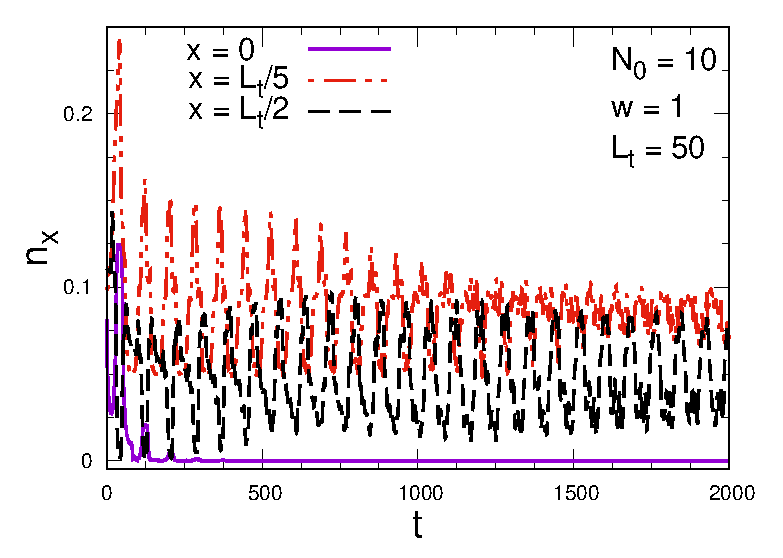
\includegraphics[width=0.65\columnwidth]{imm/nxtLt50.eps}
  \caption{ Time dependence of the particle density for systems within a
    trap of size $L_t=50$, at various spatial coordinates, $x=0$,
    $x=L_t/5=10$ and $x=L_t/2=25$, for central dissipation with $w=1$.
    The particle density $n_x$ for $x\neq 0$ are characterized by
    oscillations in the large-time regime, when $n_x$ at $x=0$ and the
    particle number have already approached their asymptotic behavior.
  }
  \label{trapnxto}
  \end{figure}
  
  
  \subsection{Large-$L_t$ scaling behavior of the time dependence}
  \label{trapscaling}
  
  
  The time dependence starting from a fixed number of particles shows
  the peculiar scaling behavior
  \begin{equation}
    R_N(t,w,L_t) \equiv {N(t)-N_{\rm asy}\over N_0-N_{\rm asy}} \approx
    A_t(t/L_t,w)\,,
    \label{rntrapn0}
  \end{equation}
  which apparently describes the whole time evolution.  This is clearly
  supported by the data reported in Figs.~\ref{trapNo} and
  \ref{trapNow01} for central dissipation with $w=1$ and initial
  particle number $N_0=10$.
  
  Note that the time scale $t\sim L_t$ may be also related to the gap of
  the fermionic Hamiltonian, for which $\Delta_{L_t} \sim
  L_t^{-z\theta}$ where $z=2$ is the dynamic exponent associated with
  the vacuum-to-superfluid transition, and $\theta=1/2$ is the universal
  trap exponent characterizing critical behaviors in the presence of
  trapping potentials~\cite{CV-09,CV-10,ACV-14,rossini2021coherent} [for generic
    power laws of the potential (\ref{potential}), $\theta=p/(p+2)$].
  
  \begin{figure}[!htb]
\centering
  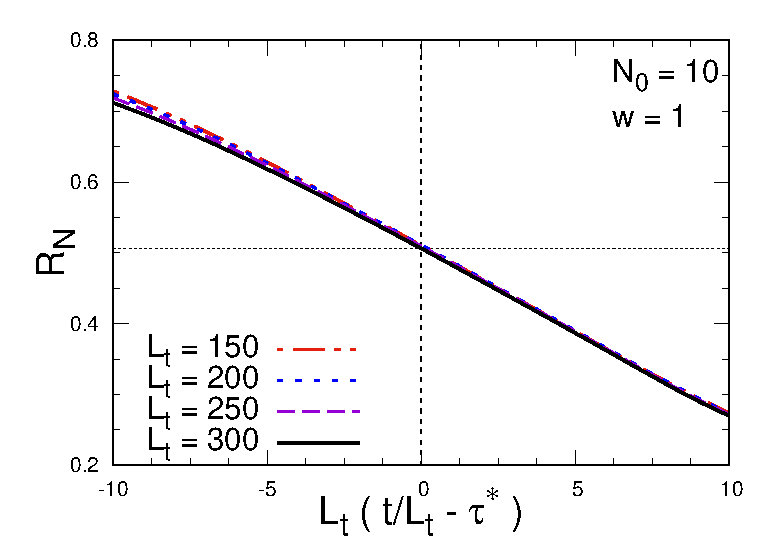
\includegraphics[width=0.65\columnwidth]{imm/crit.eps}
  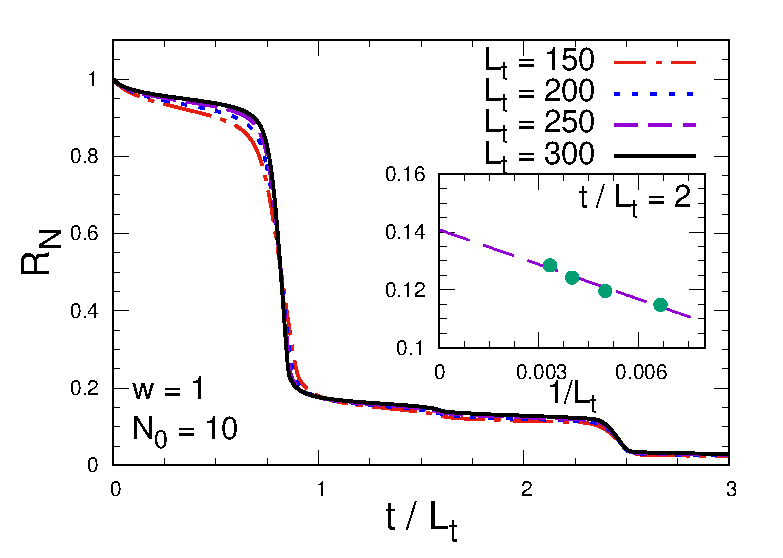
\includegraphics[width=0.65\columnwidth]{imm/RNtrapNo.eps}
  \caption{ The bottom figure shows the time evolution of the ratio
    $R_N$ versus $t/L_t$ for $w=1$, various trap sizes, keeping the
    initial number of particles $N_0=10$ fixed.  The inset shows an
    example of convergence at $t/L_t=2$.  The top figure shows the
    scaling behavior at the fast drop of the particle number, around
    $t/L_t\approx 0.8147$, described by Eq.~(\ref{atcrit}).  }
  \label{trapNo}
  \end{figure}
  
  \begin{figure}[!htb]
\centering
  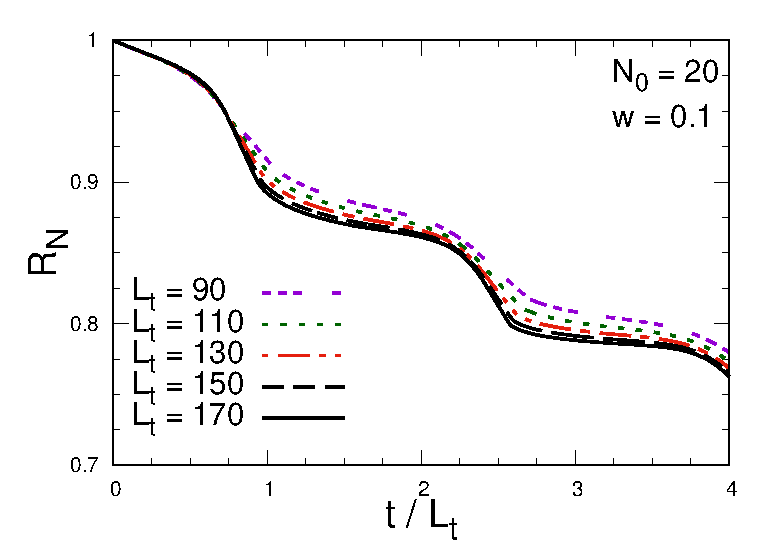
\includegraphics[width=0.65\columnwidth]{imm/RNtrapNo20w01.eps}
  \caption{The ratio $R_N$ for $w=0.1$, various trap sizes, keeping the
    initial number of particles $N_0=20$ fixed.}
  \label{trapNow01}
  \end{figure}
  
  \begin{figure}[!htb]
\centering
  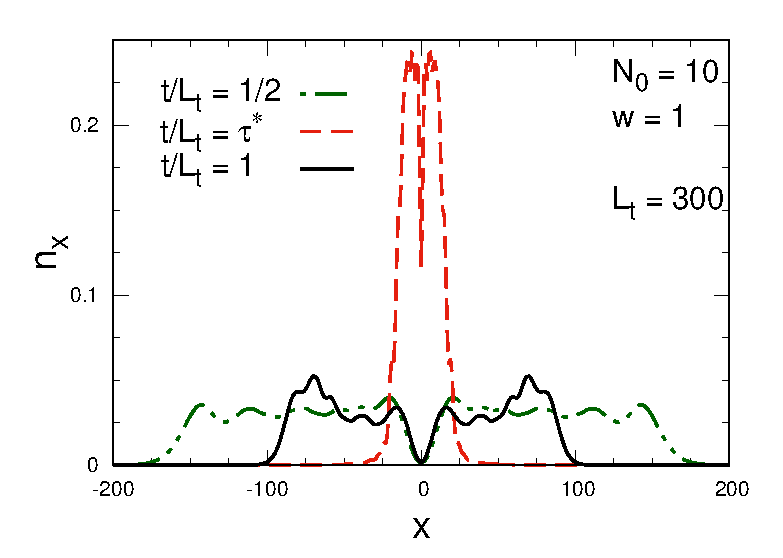
\includegraphics[width=0.65\columnwidth]{imm/nxtrap.eps}
  \caption{ Behavior of the particle density around the singularity of
    the scaling function (\ref{rntrapn0}), for $L_t=300$, central
    particle loss with $w=1$, and some values of the ratio $t/L_t$
    around the singular point $t/L_t =\tau^*\approx 0.8147$. They show
    that large drop of the particle number at $\tau^*$ is connected with
    a simultaneous large increase of the particle density at the center
    of the trap.  }
  \label{trapnx}
  \end{figure}
  
  
  
  
  
  The time scale $t\sim L_t$ characterizes the whole evolution of the
  system, up to the large-time regime, except for some small
  intermediate time intervals. Indeed, the curves shown in the bottom
  Fig.~\ref{trapNo} presents some flat regions followed by rapid
  changes.  Actually a more careful analysis, see, e.g., the top
  Fig.~\ref{trapNo}, shows that the scaling function $A_t(t/L_t,w)$
  entering Eq.~(\ref{rntrapn0}) appears to develop a singularity in the
  large-time limit, at $t/L_t = \tau^*\approx 0.8147$, so that
  \begin{equation}
    A_t(t/L_t,w) \approx f[L_t (t/L_t-\tau^*)]
    \label{atcrit}
  \end{equation}
  around $t/L_t=\tau^*$. Therefore this sharp drop of the particle
  density occurs at a time $t^* \approx L_t \tau^*$ in the large-$L_t$
  limit, and lasts for a finite time interval, i.e. it does not diverge
  when increasing $L_t$.  Some data for the behavior of the particle
  density and number around the time $\tau^*$ are shown in
  Fig.~\ref{trapnx}, where we note the significant increase of the
  particle density around $x=0$ when the singular behavior of the
  scaling function (\ref{rntrapn0}) appears.  Analogous behaviors are
  observed for generic values of $N_0$ and $w$.
  
  
  In the case we keep $N_0/L_t$ fixed, the results show a generic
  scaling behavior in terms of $t/L_t$, analogous to
  Eq.~(\ref{rntrapn0}), see for example Fig.~\ref{trapNoLt}.
  
  
  
  
  
  
  \begin{figure}[!htb]
\centering
  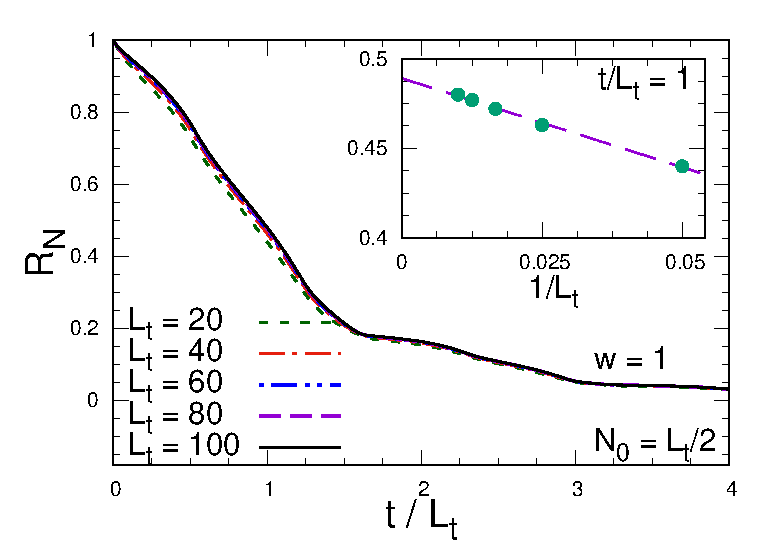
\includegraphics[width=0.65\columnwidth]{imm/RNtrapNoLt.eps}
  \caption{ Time evolution of the ratio $R_N$ versus $t/L_t$ for
    fermionic gases within harmonic traps of various size, keeping the
    ratio $N_0/L_t=1/2$ fixed, for central particle-loss dissipation with
    $w=1$. The  large-$L_t$ convergence is evident, as also shown by
    the plot reported within the inset. }
  \label{trapNoLt}
  \end{figure}
  

\section{From local to uniform dissipation: the sunburst model}

%{\bf describe a bit the model and the interplay between uniform and local dissipation 
%regime}

\begin{figure}
    \centering
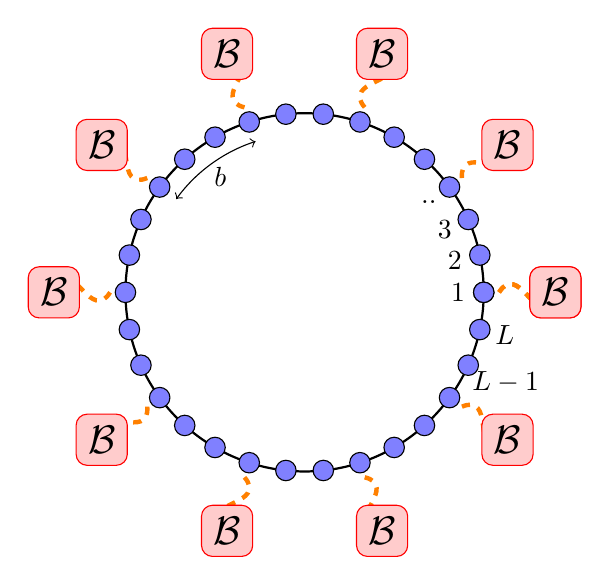
\begin{tikzpicture}[scale=0.65]
    \draw[thick] (0,0) circle (3.5cm);

    \foreach \x in {0,12,...,360}
    \filldraw [fill=blue!50] (\x:3.5cm) circle (0.2);

    \foreach \x in {0,36,...,360}
    \draw[orange, dashed, ultra thick] (\x:3.8cm) .. controls (\x+8:4.2cm) and (\x-8:4.6cm) .. (\x:4.6cm);

    \foreach \x in {0,36,...,360}
    \node[rectangle,
    draw = red,
    text = black,
    fill = red!20!white,
    rounded corners,
    minimum size=0.65cm] (r) at (\x:4.9cm) {\Large $\mathcal{B}$};

    \draw[<->] (108:3.1cm) arc
    [start angle=108,
        end angle=144,
        radius=3.1cm,
    ] ;

    \node[] (s1) at (126:2.8cm) {$b$};

    \node[] (s1) at (0:3cm) {$1$};
    \node[] (s2) at (12:3cm) {$2$};
    \node[] (s3) at (24:3cm) {$3$};
    \node[] (s4) at (36:3cm) {$..$};
    \node[] (s5) at (-12:4cm) {$L$};
    \node[] (s6) at (-24:4.3cm) {$L-1$};
\end{tikzpicture}
    \caption{Sketch of a Kitaev ring with $L=30$ qubits coupled with $n=10$ dissipators in a \textit{sunburst} geometry ($b=3$ in the figure).}
    \label{fig_sketch_sunburst_dissipation}
\end{figure}

We consider a lattice model tailored to unveil the crossover regime between the  dissipation schemes presented. We investigate a $(1+1)$-dimensional Kitaev ring with local particle-decay dissipators arranged in a \textit{sunburst} geometry~\cite{FRV-staticsunburst, FRV-timesunburst, MS-2022-sunburstquench}. The whole apparatus is sketched in Fig.~\ref{fig_sketch_sunburst_dissipation}. The open quantum system is coupled with the environment by means of $n\equiv L/b$ equally-spaced external baths, which reduce to some extent the translation invariance of the starting model.
In particular, we focus on the case of particle-decay jump
operators in the Eq.\eqref{eqlindblad}, i.e., $\hat L_x = \hat c_x$ , where fermionic 
particles are continuously removed from the site $x$. With this choice,
the Liouville operator ${\cal L}$ is quadratic in the fermionic
variables $\hat c_x$ and $\hat c_x^\dagger$ , and, in this sense, we say that the
open ring we study maintains its integrability. Most of
the results discussed in this work should preserve their
validity also for particle-pumping dissipation ( $\hat L_x = c_x^\dagger$ ),
since Eq. \eqref{eqlindblad} is still quadratic in the fermionic creation
and annihilation operators.\\

We explore different large-size limits, depending on the number of dissipators taken into account. A thorough study of the Liouvillian gap $\Delta_\lambda$ is the main focus of the first part of this section. In the second part, we examine the real-time evolution of the system, triggered by a \textit{soft quench} of a coupling constant appearing in the defining hamiltonian~\footnote{In a \textit{soft quench} the variation of the quenched parameter is attenuated down to $0$ with increasing the lattice size $L$.}. Starting the protocol in the proximity of a CQT, we study the out-of-equilibrium dynamic using RG arguments and FSS frameworks~\cite{C-1996-ScalingandRG, RV-2021-coherentanddissipativedynamicsreview}.\\

We emphasize the interplay between the unitary and dissipative dynamics and the role played by the gap $\Delta_\lambda$, extending some of the results already presented in Ref.~\cite{NRV-2019-competingdissipativeandcoherent} to our model. To outline our FSS theory, we mainly focus on the scaling properties of the critical correlations and one of the most common entanglement quantifiers, i.e., the entanglement entropy~\cite{ZMZ-2021-Renyientropiesopen}.



\subsection{Liouvillian Gap}

This section is devoted to discussing the different scaling behaviors observed for the Liouvillian gap $\Delta_\lambda$ defined in the subsection \ref{subsec_liouvilliangap}. We will consider two different limits, depending on the number of dissipation sources considered with increasing the lattice size.

%\vspace{-0.4cm}

\subsubsection{Liouvillian gap at fixed $b$}

The value of the Liouvillian gap at fixed $b$ can be computed using two different algorithm.
One, useful for small value of $b$, consists to analyze the system in the Fourier space 
the Lindblad vectorized Eq. \eqref{vecteqlindblad} whose spectrum gives the gap. 

The latter uses the third quantization technique, see details in 
Ref.~\cite{P-2008-thirdquantization}, particularly convenient for high value of the 
parameter $b$ \cite{franchi2023Liouvillian}. Without loss of generality, we will focus only
on small values of $b$, i.e. up to $b=7$, but all the results can be extended also in
the case of high $b>7$.\\

For $b=3$, the Liouville gap $\Delta_\lambda$ shows a behavior in terms of $w$ in Fig.~\ref{fig_liouvgap3b}.
At fixed $L$, we can easily distinguish two different regimes for the gap, which are separated by a bump in the gap located at $w_*(L)$. We clarify that a non-monotone trend in $\Delta_\lambda$ is not unexpected due to the presence of the \textit{quantum Zeno effect} — the dynamic of a quantum system slows down when it is frequently monitored~\cite{MS-1977-quantumzeno, HHNU-2022-Incoherentons}. Note also that both $w_*(L)$ and $\Delta_\lambda(w_*)$ vanish in the thermodynamic limit, so only the region with $w\geq w_*$ is relevant to determine the typical relaxation time of the system for large enough ring sizes. As shown in Fig.~\ref{fig_liouvgap3b}, for $w<w_*$, the gap is perfectly compatible with a linear dependence of the form

\begin{figure}[!h]
    \centering
    \includegraphics[width=8cm]{imm/gapliouv3b.pdf}
    \caption{Liouvillian gap $\Delta_\lambda$ in terms of the dissipation coupling $w$ for $b=3$ and fixed $\mu=-2$. For small $w$ and $L$ finite, the gap depends linearly on the dissipation strength as $\Delta_\lambda=w/2b$. With increasing $L$ and finite $w>0$, the Liouvillian gap approaches a different regime, which still depends linearly on $w$. In the inset, scaling corrections evaluated at $w=1$ are perfectly consistent with a $L^{-2}$ decaying. The gray straight line is drawn to guide the eye.}
    \label{fig_liouvgap3b}
\end{figure}

\begin{equation}
\Delta_\lambda(w, b)=\frac{w}{2b}\,, \quad w<w_*\,.
\label{eq_deltaL_w_smaller_w*}
\end{equation}

We have verified numerically that the above expression holds also for different values of $b\leq7$ (not shown). This equation has a clear interpretation when we rewrite $\mathbb{D}[\rho]$ in momentum space. Indeed, the full Hilbert space decomposes into the direct product of $n/2$ distinguished sectors with a dimension $4^b$. The effective coupling perceived within each sector is equal to $w/b$. If we additionally assume that the minimum contribution stemming from a single sector is $1/2$ (which is always the case for $b=1$), we get Eq.~\eqref{eq_deltaL_w_smaller_w*}.\\

On the other hand, when $w>w_*$, we observe that the gap $\Delta_\lambda$ still depends linearly on the coupling $w$, but the slope of the asymptotic straight line approached is no longer $1/2b$. We conjecture that for $w>w_*$ and sufficiently large $b$, the following expression describes the Liouvillian gap
\begin{equation}
    \Delta_\lambda(w, b)=A_\mu(b) w\,,\quad A_\mu(b)=\frac{C_\mu}{b^{3}}\,,\quad w>w_*\,,
    \label{eq_liouvillian_gap_largeL}
\end{equation}
where $C_\mu$ is a constant that only depends on the chemical potential $\mu$. Matching arguments with the boundary-dissipation cases surely prompted our guess. Indeed, when $b\propto L$, we expect to recover the leading behavior $\Delta_\lambda\sim L^{-3}$ frequently observed in the literature. Our ansatz is fully supported by the data that we have collected for $A_\mu$ in terms of $1/b^{3}$, as shown in Fig.~\ref{fig_ratelatetime} \footnote{Systematic error bars reported in the figure have been estimated from the comparison of $A_\mu(b)$ for different lattice sizes $L\geq L_{\text{min}}$ and coupling ranges $w\geq w_{\text{min}}$.}. Indeed, a straight line with a slope of $C_\mu=0.601(3)$ describes our data for all values of $b\geq3$ considered ($\chi^2/\text{ndof}=1.0$).  

\begin{figure}
    \centering
    \includegraphics[width=8cm]{imm/ratelatetime.pdf}
    \caption{Liouvillian rate coefficient $A_{\mu}(b)$ versus $b^{-3}$ with constant $\mu=-2$. For $b\geq3$, we observe that $A_{\mu}(b)$ is compatible with a power-law dependence of the form $A_{\mu}(b)=C_{\mu}/b^{3}$, where $C_{\mu}=0.601(3)$ ($\chi^2/\text{ndof}=1.0$).}
    \label{fig_ratelatetime}
\end{figure}

We also want to mention a scaling regime observed for $L\Delta_\lambda$ in terms of $w L$ when the latter quantity is kept fixed in the large size limit. In Fig.~\ref{fig_scaling_delta_apbc}, we report our data for $b=2, \mu=-3$ and $b=4, \mu=-1$.


\begin{figure}[!b]
    \centering
    \includegraphics[width=6.4cm]{imm/scalingDeltaapbc.pdf}
    \includegraphics[width=6.4cm]{imm/scalingDelta4bmuminus1.pdf}
    \caption{Scaling of $L \Delta_\lambda$ versus $w L$ for different values of $b$ and $\mu$. On the top panel, we show results for $b=2$ and $\mu=-3$, while on the bottom panel, we fix $b=4$ and $\mu=-1$. The figures show an excellent data collapse in agreement with $L^{-2}$ scaling corrections. The straight lines in the insets are drawn to guide the eye.}
    \label{fig_scaling_delta_apbc}
\end{figure}



\subsubsection{Liouvillian gap at fixed $n$}
\label{sec_liouvillian_gap_fixed_n}

Now we start to study the behavior when we keep $n=L/b$ fixed. Since the number of the
external baths scales with the system size $L$, we will apply the third quantization 
technique, cited above.

The Fig.~\ref{fig_rescaleddelta_apbc_nfixed} shows that the gap scales as  
$\Delta_\lambda\sim L^{-3}$ at fixed $w$ in the regime $w>w_*$ ($w_\star$ is the maximum
point). This scaling is correlated also to the Eq.\eqref{eq_liouvillian_gap_largeL} and
simple matching arguments.\\



\begin{figure}[!t]
    \centering
    \includegraphics[width=8cm]{imm/delantipk0bl2L3Dw.pdf}
    \caption{Plot of the rescaled gap $L^3\Delta_\lambda$ in terms of $w$ for fixed $n=2$ and $\mu=-2$.  At fixed $w$, the gap shows a nice data collapse within $L^{-1}$ scaling corrections, as provided by the inset for the case $w=1.5$. The straight line is drawn to guide the eye.}
    \label{fig_rescaleddelta_apbc_nfixed}
\end{figure}

\begin{figure}[!b]
    \centering
    \includegraphics[width=8cm]{imm/scalingDeltanfixedmuminus1.pdf}
    \caption{The figure shows the Liouvillian gap $L^2\Delta_\lambda$ versus $w$ at fixed $n=10$ for $\mu=-1$. In the inset, scaling corrections at $wL=50$ are consistent with a decay $L^{-2}$. The straight line is drawn to guide the eye.}
    \label{fig_scalingDeltanfixed}
\end{figure}

Referring to Fig.~\ref{fig_rescaleddelta_apbc_nfixed}, when $w<w_*$ the gap does not show a uniform limit for $w\to0^+$ as the maximum of $L^3\Delta_\lambda$ grows without bounds with increasing $L$. We shed some light on this peculiar trend in Fig.~\ref{fig_scalingDeltanfixed}, considering the structure of the gap in the proximity of $w=0$ at fixed $n=10$ and $\mu=-1$. In fact, the plot supports the existence of a scaling regime for $L^2\Delta_\lambda$ when $w$ is properly rescaled as $w \sim 1/L$. Scaling corrections are also compatible with a decaying $L^{-2}$, as shown in the corresponding inset. We stress again that numerical results for different values of $\mu$ do not exhibit remarkable differences. We conclude that the different scaling regimes shown by the Liouvillian gap do not depend either on $\mu$ or the quantum phase related to the Kitaev model.


\subsection{Dynamic FSS Framework}


In this section, we study the time evolution of the Kitaev ring in the proximity of a CQT. To this end, we exploit a dynamic FSS framework and use RG arguments to describe the evolution of the critical correlations. Concerning the algorithms adopted, we speed up our simulations by moving to the momentum basis every time we maintain $b$ fixed. On the other hand, when $n$ is fixed, we just monitor the evolution of the two-point correlation functions by solving a closed system of differential equations. To evolve the density matrix $\rho$ in time, we use standard $4^{\text{th}}$-order Runge-Kutta techniques with typical integration time steps of $\Delta t=0.01$.

\subsubsection{The quench protocol and the monitored observables}
\label{sec_observables}

We now present the quench protocol considered to study the time evolution of the open quantum system under scrutiny at CQTs. We prepare the system in the ground state $\ket{\Omega}$ of Eq.~\eqref{kitaev2}. The starting chemical potential $\mu_i$ is always close to the critical value $\mu_c$, meaning that $\abs{\mu_i-\mu_c}\to0$ for $L\to\infty$. At a reference time $t=0$, the ring is driven out-of-equilibrium by suddenly coupling the system with the surrounding environment and eventually quenching the chemical potential to a different value $\mu_i\to\mu_f$. In such a case, the final $\mu_f$ should always be sufficiently close to the critical point. 

We monitor the time evolution of the Kitaev ring by considering two distinguished two-point correlation functions $C(x, y, t)$ and $P(x, y, t)$, defined as
\begin{align}
	C(x, y, t)&\equiv{\rm Tr}[\rho(t)(\hat{c}^\dagger_x\hat{c}_y+\hat{c}^\dagger_y\hat{c}_x)]\,,\\
	P(x, y, t)&\equiv{\rm Tr}[\rho(t)(\hat{c}^\dagger_x\hat{c}^\dagger_y+\hat{c}_y\hat{c}_x)]\,.
    \label{eq_def_two_point_functions_C_P}
\end{align}

%%===============================================================================

\subsection{Out-of-equilibrium FSS frameworks at CQTs with $b$ fixed}
\label{sec_Out-of-equilibrium FSS at CQT}

To describe the time evolution of the system under study at CQTs, we employ RG arguments and a dynamic FSS framework~\cite{C-1996-ScalingandRG, RV-2021-coherentanddissipativedynamicsreview}. The interplay between the unitary and dissipative dynamics of a Kitaev ring subject to complete bulk dissipation ($b=1$) has already been addressed in Ref.~\cite{NRV-2019-competingdissipativeandcoherent}. The results presented in this section extend the FSS reported in that work to all the cases with fixed $b>1$, and provide a complementing discussion on the role of $\Delta_\lambda$ in such a regime. Let us first review the main ideas leading to the FSS theory that we are going to discuss.

When we consider the time evolution of an open quantum system after a quench, analogous equations are more involved given the presence of a larger number of scaling quantities and relevant perturbations. First of all, we need to introduce a pre- and a post-quench scaling field $M_{i/f}=(\mu_{i/f}-\mu_c)L^{y_\mu}$ for $\mu$. In the second place, the time variable $t$ requires a scaling field as well. The most natural guess, which also turns out to be the correct one in most cases, is to rescale $t$ with $L$ on the basis of the dynamic critical exponent $z$. We then introduce the quantity $\Theta$ defined as
\begin{equation}
    \Theta = t L^{-z}\,, \quad z=1\,,
    \label{eq_def_Theta_scaling}
\end{equation}
which is maintained constant in the FSS limit.
Since the number of particle-decay jump operators increases as $L$, we also need to soften the coupling $w$ to observe an interplay between the critical and dissipative modes. We note that the parameter $w$ plays the role of
a decay rate, namely, it is an inverse relaxation time~\cite{NRV-2019-competingdissipativeandcoherent, BP-openquantumsystembook}.
In our work hypothesis, we then suppose that $w$ should be rescaled with $L^{-z}$ to observe universal FSS relations. We introduce the scaling field $\gamma_b$ as
\begin{equation}
    \gamma_b=\frac{wL^{z}}{b}\,,\quad z=1.
    \label{def_gamma_scaling}
\end{equation}
Naturally, the prefactor $b^{-1}$ appearing in $\gamma_b$ is just a matter of convention if one restricts the analysis to just one value of $b$. However, the comparison between different values of $b$ in the FSS limit may add new valuable insights to our analyses. To compare the dissipative processes of different rings on the same footing, we assume that the effective coupling strength is $w/b$. This choice is the most natural one considering the Kitaev ring in momentum space. 

\begin{figure}
    \centering
    \includegraphics[width=7cm]{imm/Cscaling2b.pdf}
    \caption{Scaling of the two-point function $L C(X, Y)$ in terms of the scaling variable $\Theta$ for fixed $b=2$, $M_i=1$ and $\gamma_b=1$. We consider $(Y-X)/L=1/4$ and fix $x=1$, using translation invariance. In the inset, we show a zoom of the region $\Theta\in[0.35, 0.4]$. Our data clearly support the FSS laws exhibited in Eq.\eqref{eq_scaling_C}.}
    \label{fig_Cscaling2b}
\end{figure}

The universal scaling relations satisfied by the two-point functions $C$ and $P$ in Eq.~\eqref{eq_def_two_point_functions_C_P} follows
\begin{align}
    C(x, y, t) &\approx L^{-2y_c}\mathcal{C}(M_i, M_f, \{X_i\}, \Theta, \gamma_b)    \label{eq_scaling_C}\\
    P(x, y, t) &\approx L^{-2y_c}\mathcal{P}(M_i, M_f, \{X_i\}, \Theta, \gamma_b)\,,
    \label{eq_scaling_P}
\end{align}
where $y_c=1/2$ is the scaling dimension of both $\hat{c}$ and $\hat{c}^\dagger$. 
In Fig.~\ref{fig_Cscaling2b} we show the scaling of $LC(X, Y, t)$ in terms of the scaling quantity $\Theta$ for $b=2$, $M_i=1$, $M_f=-1$, and $\gamma_b=1$. The panel definitely supports the FSS laws exhibited in Eq.~\eqref{eq_scaling_C}. In the inset, we show that the amplitude of the oscillations reduces at fixed $\Theta$ and increasing $L$, roughly as $\sim L^{-1/2}$. We have checked that Eq.~\eqref{eq_scaling_P} holds also for the scaling of the RG invariant quantity $LP(X, Y, t)$ (not shown).  
\subsection{Out-of-equilibrium FSS framework at CQTs with $n$ fixed}
\label{sec_out-of-equilibrium FSS fixed n}

\begin{figure}
    \centering
    \includegraphics[width=7cm]{imm/fssnfixed2n.pdf}
    \caption{Scaling of the rescaled two-point correlation function $L C(X, Y)$ in terms of $\Theta$ for fixed of $n=2, M_i=1, M_f=3$, and $W=0.01$. We consider $Y-X=L/4$, exploiting translation invariance, and fix the first site to $x=1$ in conjunction with a dissipator. We zoom in on the domain $\Theta\in[0.35, 0.4]$ to emphasize the convergence of different curves with increasing lattice size $L$.}
    \label{fig_fss_2n_fixed}
\end{figure}

In this section, we derive a dynamic FSS framework at CQTs to study the time evolution of Eq.~\eqref{eqlindblad} when the number of the dissipators $n$ is fixed. Most of the scaling relations of the last section are still valid at fixed $n$ with straightforward generalizations. In particular, we just replace the coupling $w$ in our relations, which now represents a decay rate per unit space since $b\sim L$. As a working hypothesis, we expect the scaling field $W$, defined as
\begin{equation}
    W = w L^{z-1}\,, \quad z=1\,,
    \label{eq_def_scaling_variable_W}
\end{equation}
to be a reasonable scaling quantity in the FSS limit. 
For instance, the critical correlations satisfy scaling relations similar to the ones reported in Eq.~\eqref{eq_scaling_C}
\begin{align}
    C(x, y, t)\approx& L^{-2y_c}\mathcal{C}(M_i, M_f, \{X_i\}, \Theta, W)\\
    P(x, y, t)\approx& L^{-2y_c}\mathcal{P}
    (M_i, M_f, \{X_i\}, \Theta, W)\,.
    \label{eq_def_CP_scaling_n_fixed}
\end{align}

We verify our hypotheses in Fig.~\ref{fig_fss_2n_fixed}, showing the scaling curve for $L C(X, Y, t)$ versus the scaling variable $\Theta$ with constant $n=2, M_i=1, M_f=3, W=0.01$. We obtain a nice data collapse considering lattice sizes up to $L=256$. The oscillation amplitudes shrink with increasing $L$, converging to a universal asymptotic curve $\mathcal{C}$. The validity of Eq.~\eqref{eq_def_CP_scaling_n_fixed} has been checked also by inspecting the time evolution of $L P(X, Y, t)$ (not shown).



\begin{comment}
    
\section{Summary}

When we keep $b$ fixed, the gap $\Delta_\lambda$ is always finite and depends linearly on the dissipation strength $w$. Nonetheless, two different regimes emerge for systems of finite size. In the small $w$ region, the gap is given by $\Delta_\lambda=w/(2b)$, whereas, at large $w$ and sufficiently large $b$, it behaves as $\Delta_\lambda=w C_\mu/b^3$. The last equation always controls the gap in the large-size limit and is our starting point to deduce the scaling of such a quantity when $b\propto L$. It is worth mentioning that we also put forward a scaling regime for $L\Delta_\lambda$ as a function of $wL$, which ties together the two different regimes outlined in a smooth manner. On the other hand, when we keep the number of dissipators $n$ fixed, the gap vanishes as $\sim L^{-3}$ at large $L$. Addressing the structure of the gap at small $w$, we find a scaling regime for $L^2\Delta_\lambda$ in terms of $wL$, which is closely related to the presence of a non-uniform convergence of $L^3\Delta_\lambda$ in the limit $w\to0^+$.\\

We develop a dynamic FSS regime at CQTs to describe the time evolution of the Kitaev model under investigation. At fixed $b$, our results extend the FSS theory of Ref.~\cite{NRV-2019-competingdissipativeandcoherent} to the cases with $b>1$. As a working hypothesis, we suppose that the scaling variable associated with the relevant coupling $w$ is $\gamma_b=wL^{z}/b$. Our numerical results for the two-point correlation functions fully support this ansatz. When the number of dissipators $n$ is fixed, the FSS theory outlined at fixed $b$ generalizes straightforwardly after replacing $\gamma_b$ with $W=wL^{z-1}$. 

%In the last section, we analyze the interplay between the Liouvillian gap $\Delta_\lambda$ and the gap related to the Kitaev ring $\Delta$ in the FSS limit. In particular, we take into account the short- and long-time regimes, focusing on how they join together in the FSS limit. When $b$ is fixed, we observe that the link between the two regimes is smooth, whereas, at fixed $n$, the two regions can be easily distinguished given the presence of different power-law scalings for the gaps $\Delta$ and $\Delta_\lambda$. 
\end{comment}




\section{Thermal-bath effects in quantum quenches}

%\subsection{Kitaev fermionic wires and thermal baths}
\label{modbath}

\subsection{The fermionic Kitaev chain}
\label{kitaevmod}

We consider fermionic Kitaev wires of $L$ sites with open boundary
conditions, whose quantum unitary dynamics is driven by the
Hamiltonian~\cite{Kitaev-01}
\begin{equation}
  \hat H_{\rm K} = - J \sum_{x=1}^{L-1} \big( \hat c_x^\dagger \hat
  c_{x+1}^{\phantom\dagger} +
  \hat c_x^\dagger \hat c_{x+1}^\dagger+{\rm h.c.}
  \big) - \mu \sum_{x=1}^L \hat n_x ,
  \label{kitaev2}
\end{equation}
where $\hat c_x$ is the fermionic annihilation operator associated
with the site $x$ of the chain, $\hat n_x\equiv \hat
c_x^\dagger \hat c_x^{\phantom\dagger}$ is the particle density
operator.  In the following we assume $J$ as the energy scale, thus we
set $J=1$.

The Hamiltonian~\eqref{kitaev2} can be mapped into a quantum Ising
chain, by means of the Jordan-Wigner transformation, see, e.g.,
Ref.~\cite{Sachdev-book}.  The corresponding spin model is the
quantum Ising chain with open boundary conditions, i.e.
\begin{equation}
  \hat H_{\rm Is} = -\sum_{x=1}^{L-1} \hat \sigma^{(1)}_x \hat
  \sigma^{(1)}_{x+1} - g\, \sum_{x=1}^L \hat \sigma^{(3)}_x,
  \label{isham}
\end{equation}
$\hat \sigma^{(k)}_x$ being the Pauli matrices and $g=-\mu/2$.  In the
following we prefer to stick with the Kitaev quantum wire, because the
thermal baths and observables that we consider are best defined within
the fermionic model. However, the general scaling scenarios that will
emerge apply to both models.

The Kitaev model undergoes a CQT at $\mu=\mu_c = -2$ (corresponding to
$g=g_c=1$ in the quantum Ising chain), between a disordered quantum
phase for $\mu<\mu_c$ (corresponding to $g>1$) and an ordered quantum
phase for $|\mu|<|\mu_c|$ (corresponding to $|g|<1$). Thus, we define
\begin{equation}
  w = \mu - \mu_c = \mu + 2,
  \label{wdef}
\end{equation}
so that one can easily see the correspondence between the Kitaev
Hamiltonian (\ref{kitaev2}) and the generic one reported in
Eq.~(\ref{qudef}), i.e. $\hat{H}_c$ corresponds to the Hamiltonian
(\ref{kitaev2}) for $\mu=\mu_c$, and $\hat{H}_p=-\sum_{x=1}^L \hat
n_x$.  The continuous transition at $w=w_c$ belongs to the
two-dimensional Ising universality class~\cite{Sachdev-book,RV-21},
characterized by the length-scale critical exponent $\nu=1$, related
to the RG dimension $y_w = 1/\nu=1$ of the Hamiltonian parameter
$w$. This implies that, approaching the critical point, the length
scale $\xi$ of the critical quantum fluctuations diverges as $\xi \sim
|w|^{-\nu}$. The dynamic exponent $z=1$ associated with the unitary
quantum dynamics can be obtained from the power law
$\Delta\sim\xi^{-z}$ of the vanishing gap with increasing $\xi$.
Moreover, the RG dimension of the fermionic operators $\hat c_j$ and
$\hat c^\dagger_j$ at the CQT is $y_c = 1/2$, and that of the particle
density operator $\hat n_x$ is $y_n = 1$~\cite{Sachdev-book,RV-21}.


\subsection{Modelization of the thermal bath}
\label{thebath}

In our study we consider a modelization of interaction with a thermal
bath within the Lindblad master equation (\ref{Lindblad}), whose
asymptotic large-time behavior leads to a Gibbs density matrix at a
given finite temperature $T$. In particular, we consider the proposal
developed in Ref.~\cite{DR-21} which applies to quantum models
described by quadratic Hamiltonians, such as that of the fermionic
Kitaev wires. This provides a relatively simple modelization of a
thermal bath leading to thermalization in the large-time limit of the
corresponding Lindblad master equation for the density matrix of the
system.

The Kitaev Hamiltonian (\ref{kitaev2}) with open boundary conditions
can be diagonalized in the Nambu field space by a Bogoliubov
transformation, see e.g. Refs.~\cite{Pfeuty-70,BR-book,DR-21}, so that
we can rewrite it as
\begin{equation}
\hat{H}_{\rm K}=\sum_{k=1}^L\,\omega_k \,\hat b^\dagger_k\, \hat b_k,
  \label{Hdiag}
\end{equation}
where $\omega_k$ are values of the spectrum of the Bogoliubov
eigenoperators $\hat b_k$ (we are neglecting an irrelevant constant
term). Note that both $\omega_k$ and $\hat b_k$ depend on the
Hamiltonian parameter $\mu$.  The relation between the fermionic
operators $\hat{c}_x$ and the Bogoliubov eigenoperators $\hat{b}_k$
can be generally written as~\cite{Pfeuty-70,BR-book,DR-21}
\begin{equation}
  \label{transBogol}
  \hat c_x = \sum_{k=1}^L A_{xk} \,\hat{b}_k + B_{xk}
  \,\hat{b}_k^\dagger,
\end{equation}
where $A$ and $B$ are appropriate $L\times L$ matrices depending on
$\mu$.  Following Refs.~\cite{DR-21,PCR-22}, we write the dissipator
$\mathbb{D}_T[\rho]$ in the Lindblad master equation (\ref{Lindblad})
in terms of the Bogoliubov eigenoperators as
\begin{eqnarray}
  \mathbb{D}_T[\rho] &=&
\sum_k [1-f(\omega_k,T)]
\left( 2 \,\hat{b}_k\,\rho\,\hat{b}_k^\dagger - 
\{\hat{b}_k^\dagger\hat{b}_k,\rho\}\right)  \nonumber\\
&+&
\sum_k f(\omega_k,T)
\left( 2 \,\hat{b}_k^\dagger\,\rho\,\hat{b}_k - 
\{\hat{b}_k\hat{b}_k^\dagger,\rho\}\right), \label{Dtrho}
\end{eqnarray}
where
\begin{equation}
  f(\omega_k,T) = \left( 1 + e^{\omega_k/T}\right)^{-1}.
  \label{fomt}
\end{equation}
When using this homogeneous dissipator term, the Lindblad master
equation (\ref{Lindblad}) ensures the asymptotic large-time
thermalization~\cite{DR-21}. Therefore,
\begin{eqnarray}
  &&\lim_{t\to\infty} \rho(t)  = \rho_t(w,T), \label{asyrho}\\
&&\rho_t(w,T) = \sum_n e^{-E_n(w)/T}|\Phi_n, w\rangle \langle \Phi_n, w|,
 \qquad \label{termrho}
\end{eqnarray}
where $\rho_t(w,T)$ is the density matrix representing the thermal
state, $E_n(w)$ and $|\Phi_n, w\rangle$ are the eigenvalues and
eigenstates of $\hat{H}(w)$.  The asymptotic approach to the thermal
distribution is controlled by the decay-rate parameter
$\gamma$~\cite{DR-21}. Indeed the Liouvillian gap $\Delta_{\cal L}$
that controls the exponential approach to the asymptotic stationary
state of the Lindblad equation is proportional to the decay rate
$\gamma$, i.e.
\begin{equation}
  \Delta_{\cal L}\sim \gamma.
  \label{deltal}
  \end{equation}

The above modelization of thermal baths provides a useful theoretical
laboratory to investigate issues related to the out-of-equilibrium
dynamics in the presence of thermal baths. Its derivation has
been thoroughly discussed in Ref.~\cite{DR-21}. We also mention that it
has been employed in Refs.~\cite{PCR-22,BD-23}.  Some details of the
computations using the Lindblad master equation (\ref{Lindblad}) with
the dissipator (\ref{Dtrho}) are reported in the appendix.


\subsection{Quantum-quench protocols}
\label{proto}

As already anticipated in Sec.~\ref{intro}, we consider two protocols,
differing for the absence or presence of the contact with the thermal
bath during the quantum evolution after quenching, giving respectively
rise to unitary or dissipative dynamics after quenching. We call them
{\em unitary} and {\em dissipative} QQ protocols, respectively.

\begin{itemize}

\item {\em Unitary} QQ protocol: In this simplest QQ protocol the role
  of the thermal bath is limited to that of preparing the initial
  Gibbs state $\rho_t(w_i,T)$ at $t=0$, reported in
  Eq.~(\ref{rhoi}). This can be obtained by keeping the thermal bath
  in contact with the system for a sufficiently long time $t_{\rm th}$, i.e
  $t_{\rm th}\gg \gamma^{-1}$. Then at $t=0$ the Hamiltonian parameter is
  instantaneously quenched from $w_i<0$ to $w\ge 0$ and the thermal
  bath is removed, so that the subsequent time evolution is that of a
  closed fermionic wire, i.e.  it is unitary and only driven by the
  Hamiltonian of the system, cf. Eq.~(\ref{firstprot}).

\item {\em Dissipative} QQ protocol: The quantum evolution starts from
  the same initial Gibbs state $\rho_t(w_i,T)$, but the thermal bath
  is maintained in contact with the system after the QQ from $w_i<0$
  to $w\ge 0$, at $t=0$.  Therefore, the quantum evolution for $t>0$
  is driven by the Lindblad master equation (\ref{Lindblad}) with the
  dissipator term (\ref{Dtrho}). Note that this dynamic protocol
  entails a further time scale $\tau = \gamma^{-1}$, characterizing
  the asymptotic exponential approach to the large-time stationary
  Gibbs state associated with the Hamiltonian $\hat{H}(w)$ and
  temperature $T$.

\end{itemize}


\subsection{Observables monitoring the time evolution}
\label{obs}


To characterize the dynamic properties of the quantum evolution after
the QQ at $t=0$, we consider the subtracted particle-density average
\begin{eqnarray}
n_s(t,L) = {1\over L} {\rm Tr} \left[ \rho(t) \sum_{x=1}^L \hat{n}_x \right]
- n_c(L),
 \label{ddef}
\end{eqnarray}
 where $n_c(L)$ is the ground-state energy density of the Kitaev wire
 of size $L$ at the critical point $w_c=0$ (in the infinite-size limit
 $n_c= 1/2 - 1/\pi$~\cite{Pfeuty-70}). Note that the particle density
 operator $\hat{n}_x$ and the transverse spin component
 $\hat\sigma_x^{(3)}$ of the quantum Ising chain (\ref{isham}) are
 trivially related, indeed $\hat{\sigma}_x^{(3)} = 2 \hat{n}_x$.  In
 the definition of $n_s$, the subtraction of $n_c(L)$ simplifies the
 scaling behavior of $n_s(t,L)$ within the critical regime, cancelling
 the leading analytical behavior~\cite{CPV-14,RV-21}. To monitor the
 spatial correlations, we also consider
\begin{eqnarray}
P(x,y,t) & \!\! = \!\! & {\rm Tr}[\rho(t)\,(\hat c_x^\dagger 
\hat c_{y}^\dagger +
    \hat c_{y} \hat c_{x})],\label{ptf}\\ 
C(x,y,t) & \!\! = \!\! & {\rm Tr}[\rho(t)\, (\hat c_x^\dagger \hat c_{y} 
+ \hat
    c_{y}^\dagger \hat c_{x})].\label{gtf} 
\end{eqnarray}

Some details on the computation of the above quantities during the
time evolution of the QQ protocols are reported in the appendix.


\subsection{Out-of-equilibrium scaling}
\label{scabeh}

We now discuss the out-of-equilibrium behaviors arising from the QQ
protocols outlined in Sec.~\ref{proto}.  We show that they develop
OFSS behaviors where the effects of the thermal baths are taken into
account by appropriate extensions of the out-of-equilibrium
zero-temperature scaling laws describing soft QQs in
closed systems within their critical regime, already put foward by
earlier works~\cite{PRV-18,RV-21}.

\begin{figure}[!htb]
\centering
  \includegraphics[width=0.6\columnwidth]{imm/NT2l60diffglog.pdf}
  \caption{The quantum evolution of the subtracted particle density
    $n_s(t)$, cf. Eq.~(\ref{ddef}), for the dissipative QQ protocol
    entailing a dissipative dynamics after the QQ at $t=0$ of the
    Hamiltonian parameter $w$, describing the persistent interaction
    with the thermal bath, cf.  Eqs.~(\ref{Lindblad}) and
    (\ref{Dtrho}).  These curves refer to a system of size $L=60$,
    temperature $T=2$ of the thermal bath, quenching from $w_i=-0.01$
    to $w=0$, and various values of the decay rate $\gamma$ (the case
    $\gamma=0$ corresponds to the evolution of the close system).  We
    plot the difference $n_s(t,L,T) - n_{s,{\rm eq}}(L,T)$ which is
    expected to vanish in the large-time limit.  In this figure and in
    the following ones, the unity that we use are such that
    $\hslash=1$, $k_B=1$, and $J=1$.}
  \label{plainns}
\end{figure}



The OFSS behaviors that we put forward for QQ protocols considered are
verified by numerical computations for the fermionic Kitaev wire up to
relatively large sizes. See the appendix for details on such
calculations.

As a preliminary example of out-of-equilibriun QQ
behaviors that we want to address, in Fig.~\ref{plainns} we show some
results for the quantum evolution of the subtracted particle density
(\ref{ddef}) along the dissipative protocol outlined in
Sec.~\ref{proto}, after quenching a fermionic Kitaev wire of size
$L=60$, from $w_i=-0.01$ to $w=0$, in the presence of a thermal bath
at a temperature $T=2$, and various values of the decay rate $\gamma$.
The quantum evolution turns out to have a significant dependence on
the decay-rate parameter $\gamma$ that characterized the interactions
between the system and the thermal bath. Indeed, the curves of the
substracted particle density appear to approach its equilibrium value
$n_{s,{\rm eq}}(w=0,T=2)\approx 0.0004601...$ (while at $t=0$ we have
$n_{s,{\rm eq}}(w=w_i,T=2) \approx 0.126598...$), faster and faster
with increasing $\gamma$, actually exponentially as $\exp(-t/\tau)$
with $\tau\sim\gamma^{-1}$, conferming the role of decay rate of the
parameter $\gamma$ within the Lindblad master equation,
cf. Eq.~(\ref{deltal}). Analogous results are obtained for other
observables, such as fermionic correlation functions defined in
Sec.~\ref{obs}. In the following we put forward an out-of-equilibrium
scaling theory for these out-of-equilibrium phenomena within the
quantum critical regime.




\subsubsection{Zero-temperature scaling in quantum quenches}
\label{zeroT}

We now provide a brief summary of the out-of-equilibrium scaling
theory for close systems, describing QQ protocols within the critical
regime~\cite{PRV-18,RV-21}. The initial state is the ground state
associated with an initial value $w_i<0$, and, after the instantaneous
quench at $t=0$ from $w_i$ to $w$, the quantum evolution is driven by
the Schr\"odinger equation.

Out-of-equilibrium scaling laws can be obtained by extending those
valid at equilibrium, allowing for a time dependence essentially
controlled by the time scaling variable $\Theta \sim t\,\Delta$, which
is obtained by assuming that the relevant time scale of the critical
modes is proportional to the inverse energy difference $\Delta$ of the
lowest states. We refer to Ref.~\cite{RV-21} for a through
presentation of the scaling arguments leading to the asymptotic OFSS
behaviors.

Let us consider the out-of-equilibrium evolution (after quenching) of
generic observables, such as the expectation value $O$ at time $t$ of
a local operator $\hat{O}({\bm x})$ and its fixed-time correlations
$G_O=\langle \hat{O}({\bm x}) \hat{O}({\bm y})\rangle$. The general
working hypothesis underlying out-of-equilibrium FSS frameworks is
that the expectation value of $\hat{O}({\bm x})$ and its correlation
functions obey asymptotic homogeneous scaling laws~\cite{RV-21}, such
as
\begin{eqnarray}
O(t, {\bm x}, L, w_i, w) \approx  b^{-y_o} {\cal O}(t/b^z,
{\bm x}/b, L/b, b^{y_w} w_i, b^{y_w} w),\quad
    \label{Oscaquefss0}
\end{eqnarray}
  where $b$ is an arbitrary (large) length scale, $y_o$ is the RG
  dimension of the local operator $\hat{O}_{\bm x}$ and the RG
  exponents $y_w$ and $z$ are determined by the universality class of
  the CQT (they are the RG dimensions of the Hamiltonian parameter $w$
  and the temperature $T$, respectively). Thus both the initial and
  final values of $w$, i.e.  $w_i$ and $w$, take the same RG exponent
  $y_w$, being coupled to the RG perturbation ${\hat H}_p$ within the
  Hamiltonian. Note that we do not assume translation invariance,
  which is generally broken by the presence of boundaries, such as
  those arising from open boundary conditions.
  
 
OFSS can be straightforwardly derived by fixing $b=L$ in the above
homogenous scaling law. Then, we expect the OFSS of the expectation
value $O$ of a generic local operator $\hat{O}_{\bm x}$, of its
spatial average $\hat{O}_a =L^{-d}\sum_{\bm x}\hat{O}_{\bm x}$, and
its two-point correlation function $G_O$, develop the asymptotic OFSS
behavior~\cite{PRV-18,RV-21}
\begin{eqnarray}
  && O(t, {\bm x}, L, w_i, w) \, \approx \, L^{-y_o} \,
  {\cal O}(\Theta, {\bm X}, \Phi_i, \Phi),
\nonumber\\
  && O_a(t, L, w_i, w) \, \approx \, L^{-y_o} \, {\cal O}_a(\Theta,
\Phi_i, \Phi),   \label{Oscaquefss}\\
  && G_{O}(t, {\bm x}_1, {\bm x}_2, L,
  w_i, w) \, \approx \, L^{-2y_o} \, {\cal G}_{O}(\Theta, {\bm X}_1,
  {\bm X}_2, \Phi_i, \Phi), \nonumber
\end{eqnarray}
where the scaling variables appearing in the scaling functions ${\cal
  O}$, ${\cal O}_a$, and ${\cal G}_O$ are defined as
\begin{equation}
  \Theta\equiv\frac{t}{L^z},\;\; {\bm X}_i \equiv \frac{{\bm x}_i}{L},\;\;
  \Phi_{i} \equiv
L^{y_w} \, w_i , \;\; \Phi \equiv L^{y_w} \,w.
  \label{scalvarque}
\end{equation}
The OFSS limit is obtained in the large-$L$ and large-$t$ limit
keeping the above scaling variables fixed. These conditions ensure
that the system remains within the universal critical regime during
the quantum evolution.  Note that in the scaling law
(\ref{scalvarque}) the dynamic features are essentially encoded in the
time dependence of the scaling variable $\Theta\sim t\,\Delta$.  The
other features, in particular when $w_i=w$, are analogous to those
arising from equilibrium FSS at CQTs~\cite{CPV-14,RV-21}, where the
argument $\Phi=L^{y_w} w$ of the scaling functions is controlled by
the RG dimension $y_w$ of the relevant parameters $w$ at the RG fixed
point associated with the CQT.


The above OFSS equations can be straightforwardly applied to the
observables defined in Sec.~\ref{obs}, after a quench from $w_i$ to
$w$ at $t=0$, keeping into account that the RG dimension of the
subtracted particle density is $y_n = 1$, and that of the fermionic
operator $\hat c_x$ is $y_c=1/2$.  Note that the dominant analytical
contributions to the particle density~\cite{CPV-14,RV-21} coming from
the analytical background are canceled in the difference $n_s$ defined
in Eq.~(\ref{ddef}), whose leading asymptotic behavior arises from the
quantum critical modes, therefore it is analogous to that of $O_a$ in
Eq.~(\ref{Oscaquefss}), with $y_o=y_n$.  Analogously one can apply the
OFSS in Eq.~(\ref{Oscaquefss}) to observables and correlation
functions constructed with the spin operators of the quantum spin
chain (\ref{isham}).  The OFSS functions are expected to be universal
with respect to the microscopic details of the model, apart from
nonuniversal multiplicative rescaling and normalizations of its
arguments.  Within isolated fermionc Kitaev wires and quantum Ising
chains, the OFSS arising from soft QQs has been verified by numerical
computations for various boundary conditions, and also along their
quantum first-order transition line~\cite{PRV-18,RV-21}.





The OFSS limit is expected to be approached with power-law suppressed
corrections.  There are various sources of scaling corrections when
approaching the OFSS. Of course, they include those that are already
present at equilibrium. In particular, the irrelevant RG perturbations
are sources of scaling corrections for the asymptotic behavior of the
free-energy density~\cite{PV-02,RV-21}.  In the case of
one-dimensional quantum systems undergoing CQTs belonging to the
two-dimensional Ising universality class, the leading scaling
corrections from irrelevant RG perturbations are suppressed as
$L^{-\omega}$ with $\omega=2$~\cite{CHPV-02,CPV-14}. However, other
contributions may become more relevant~\cite{PV-02,CPV-14,RV-21}, such
as those arising from the presence of analytical backgrounds, from the
presence of boundaries (which generally gives rise to $O(1/L)$
corrections), and, in the case of correlation functions, from RG
mixings of the source fields [this for example happens in the case of
  the correlation functions of the fermionic field $\hat{c}_x$, for
  which corrections are $O(1/L)$].  These scaling corrections have
been confirmed by numerical results~\cite{CPV-14,RV-21}. Therefore, we
expect that the asymptotic OFSS of fermionic Kitaev wires and quantum
Ising chains with open boundary conditions is generally approached
with $O(1/L)$ corrections.




\subsubsection{OFSS along the unitary QQ protocol}
\label{scalprota}



For the simplest unitary protocol reported in Sec.~\ref{proto}, where
the quantum evolution is that of the isolated fermionic wire, the
request that the dynamics remains within the critical regime implies
that the temperature of the initial Gibbs state must be appropriately
suppressed in the large-$L$ OFSS limit, to obtain a nontrivial
out-of-equilibrium critical limit.  This is analogous to what happens
within the equilibrium FSS, where one introduces the scaling
variable~\cite{SGCS-97,Sachdev-book,RV-21}
\begin{equation}
  \Xi \equiv L^z T,
 \label{Xidef}
\end{equation}
to allow for a nonzero temperature in the FSS of the observables.
Therefore, like equilibrium FSS, we conjecture that the temperature of
the initial Gibbs state enters the OFSS associated with the unitary QQ
protocol by adding a further dependence on $\Xi$ in the scaling
functions (\ref{Oscaquefss}).  In other words, a nontrivial asymptotic
OFSS limit is expected to be realized in the large-$L$ and large-$t$
limits keeping also $\Xi$ fixed, beside the scaling variables already
defined in Eq.~(\ref{scalvarque}).  Therefore, we expect that the OFSS
of standard QQ protocols starting from ground states,
cf. Eq.~(\ref{Oscaquefss}), changes into
\begin{eqnarray}
   O(t, {\bm x}, L, w_i, w, T) \, \approx \, L^{-y_o} \, {\cal
    O}(\Theta, {\bm X}, \Phi_i, \Phi, \Xi),
    \label{Oscaquefssa}
\end{eqnarray}
and analogously for its spatial average $O_a$ and the correlation
function $G_O$.

\begin{figure}[!htb]
\centering
  \includegraphics[width=0.6\columnwidth]{imm/LPk-1q0e100g0.pdf}
  \includegraphics[width=0.6\columnwidth]{imm/LNk-1q0e100g0.pdf}
  \caption{OFSS behavior of the subtracted particle density (bottom)
    and the fermionic correlation function $P(x=L/3,y=2L/3,t)$,
    cf. Eq.~(\ref{ptf}), arising from the unitary QQ protocol, for
    various lattice sizes $L$, at fixed $\Xi=L^z T =1$,
    $\Phi_i=L^{y_w} w_i=-1$ and $\Phi=L^{y_w} w=0$, versus the time
    scaling variable $\Theta=t/L^z$.  These computations nicely
    support the OFSS behaviors reported in
    Eq.~(\ref{Oscaquefssa}). The inset of the bottom figure shows that
    the approach to the OFSS limit is consistent with $O(1/L)$
    corrections.  Analogous results are obtained for other values of
    the scaling variables.}
  \label{protares}
\end{figure}


The numerical analysis for the fermionic Kitaev wire under the unitary
protocol fully support to this OFSS, obtained by extending the QQ FSS
behaviors of closed systems starting from an initial ground
state. This is clearly demonstrated by the curves reported in
Fig.~\ref{protares}, associated with the quantum evolutions of the
subtracted particle density $n_s(t)$ and the fermionic correlation
$P(x,y,t)$ (the other fermionic correlation $C(x,y,t)$ develops an
analogous OFSS).



\subsubsection{OFSS along the dissipative QQ protocol}
\label{scalprotb}

We now discuss the dynamics arising from the dissipative protocol
outlined in Sec.~\ref{proto}, when the quantum evolution after
quenching is described by the Lindblad master equation
(\ref{Lindblad}) with the thermal-like dissipator (\ref{Dtrho}), to
modelize the interaction with a thermal bath characterized by a
temperature $T$ (which does not change after quenching)
and decay rate $\gamma$.

\begin{figure}[!htb]
\centering
  \includegraphics[width=0.6\columnwidth]{imm/LNeqXik0.pdf}
  \caption{ Equilibrium FSS of the subtracted particle density
    $n_{s,{\rm eq}}$ at the critical point $w=0$, versus the rescaled
    temperature $\Xi=L^z T$. With increasing $L$, the data show the
    expected convergence to the equilibrium FSS reported in
    Eq.~(\ref{nseqsca}) with $y_n=1$. }
  \label{eqns}
\end{figure}

  
\begin{figure}[!htb]
\centering
  \includegraphics[width=0.6\columnwidth]{imm/LNk-1q0e100t100g1000.pdf}
  \caption{Quantum evolution of the subtracted particle density
    arising from the dissipative QQ protocol, when rescaling all
    quantities involved in the quench protocol, except for the decay
    rate $\gamma$. With increasing $L$, the curves appear to approach
    the equilibrium FSS value at finite temperature (where the
    temperature dependence enters through the scaling variable
    $\Xi=L^z T$) faster and faster, reflecting a nonuniform
    convergence for any $\Theta>0$. The dashed line shows the
    equilibrium value of $n_s$ for $\Phi=0$ and $\Xi=1$, which is
    asymptotically approached by the various curves.  }
  \label{protbresgamma}
\end{figure}



We expect that the temperature $T$ of the thermal bath must be
rescaled as in the case of the unitary QQ protocol, i.e. we must
consider again the associated scaling variable $\Xi$ already defined
in Eq.~(\ref{Xidef}).  However, since the QQ moves the system
out-of-equilibrium, also the decay rate $\gamma$, and corresponding
time scale $\tau=\gamma^{-1}$, associated with the interactions with
the thermal bath is expected to play a relevant role to establish a
corresponding nontrivial OFSS limit.  This was already noted in
Ref.~\cite{BD-23} in the analysis of dynamic protocols entailing the
variation of the temperature at the critical point.

When keeping $\tau$ constant in the FSS limit where the
scaling variable $\Theta=t/L^z$ is kept fixed, in the large-$L$ limit
we have eventually that
\begin{equation}
  t = \Theta \, L^z \gg \tau,
  \label{tggtau}
  \end{equation}
which is the condition ensuring thermalization for any finite value
$\Theta>0$. Therefore, when keeping $\tau$ fixed, the quantum
evolution is not expected to develop a nontrivial OFSS limit. Indeed,
in the large-$L$ limit, the system turns out to suddenly approach an
equilibrium Gibbs state (associated with the Hamiltonian parameter $w$
and temperature $T$) with respect to the rescaled time $\Theta$,
without any further relevant evolution of the system for any
$\Theta>0$.  Therefore, if the temperature is rescaled by keeping
$\Xi=L^z T$ fixed, we must recover the equilibrium FSS behavior in the
presence of a thermal bath at temperature $T$, such as that associated
with the subtracted particle density~\cite{CPV-14,RV-21}
\begin{equation}
  n_{s,{\rm eq}}(w,L,T) \approx L^{-y_n} {\cal N}(\Phi,\Xi),
  \label{nseqsca}
  \end{equation}
where $\Phi=L^{y_w} w$, and the temperature dependence enters through
the associated scaling variable $\Xi=L^z T$.  In Fig.~\ref{eqns} we
show some equilibrium data at the critical point $w=\Phi=0$, versus
$\Xi$, showing the approach to the asymptotic large-$L$ equilibrium
FSS (\ref{nseqsca}).  The realization of the equilibrium FSS within
the QQ protocol at fixed $\gamma$ is demonstrated by the plots
reported in Fig.~\ref{protbresgamma}, which show the somewhat trivial
convergence toward the equilibrium FSS for any finite $\Theta>0$.

The above results suggest that also the the decay rate $\gamma$ of the
system-bath interactions must be rescaled to observe a nontrivial OFSS
limit as a function of the time scaling variable $\Theta$, to create
the conditions for a balanced competition between the critical
Hamiltonian driving and the interactions with the thermal bath. As
already put forward in the case of other homogeneous dissipative terms
in the Lindblad equation~\cite{NRV-19-cd,RV-20-kz,TV-21,RV-21,FT-23},
for example associated with particle-decay or particle-pumping
dissipative mechanisms, a nontrivial OFSS limit is obtained by
rescaling the decay rate of the dissipative term, so that the scaling
variable
\begin{equation}
  \Gamma \equiv L^z \gamma \sim \gamma/\Delta
  \label{gammadef}
\end{equation}
is kept fixed in the OFSS limit, where $\Delta$ is the energy
difference of the lowest eigenstates of $\hat{H}(w)$ at the critical
point $w=w_c=0$.  Then an OFSS behavior emerges from the nontrivial
competition between the critical unitary dynamics and the dissipative
driving arising from the thermal bath.


\begin{figure}[!htb]
    \centering
      \includegraphics[width=0.45\columnwidth]{imm/LCk-1q0e100t100S10000.pdf}
      \includegraphics[width=0.45\columnwidth]{imm/LPk-1q0e100t100S10000.pdf}
        \includegraphics[width=0.45\columnwidth]{imm/LNk-1q0e100t100S10000.pdf}
        \caption{Quantum evolutions along the dissipative protocol, fully
          supporting the OFSS reported in Eqs.~(\ref{Oscaquefssprotb1})
          and (\ref{Oscaquefssprotb2}). We report curves for $L\,n_s$
          (bottom), $L\,P(x=L/3,y=2L/3,t)$ (middle), and
          $C(x=L/3,y=2L/3,t)$ (top), for various values of $L$, at fixed
          $\Phi_i=-1$, $\Phi=0$, $\Xi=1$, and two values of
          $\Gamma=L^z\gamma$, i.e.  $\Gamma=1,\,10$ (except for the top
          figure where we only report data for $\Gamma=10$ to ensure a
          good readability).  The inset of the top figure shows that the
          OFSS is approached with $O(1/L)$ corrections. Analogous results
          are obtained for other values of the scaling variables. }
      \label{protbresgammaresc}
\end{figure}

In conclusion, on the basis of the above scaling arguments, the OFSS
arising from the dissipative QQ protocols in the presence of a thermal
bath is expected to be given by
\begin{eqnarray}
   O_a(t, L, w_i, w, T, \gamma) \, \approx \, L^{-y_o} \,
  {\cal O}_a(\Theta, \Phi_i, \Phi, \Xi, \Gamma),\quad
  \label{Oscaquefssprotb1}
\end{eqnarray}
and
\begin{eqnarray}
&& G_{O}(t, {\bm x}_1, {\bm x}_2, L, w_i, w, T, \gamma)  \, \approx
    \label{Oscaquefssprotb2} \\
    &&\qquad\qquad
     L^{-2y_o} \, {\cal G}_{O}(\Theta, {\bm X}_1, {\bm X}_2, \Phi_i,
    \Phi, \Xi, \Gamma). \qquad \nonumber
\end{eqnarray}
In the large-$\Gamma$ limit the above OFFS behaviors at fixed $\Xi$ is
expected to approach the corresponding equilibrium FSS, faster and
faster in terms of $\Theta$, matching the behavior at finite $\gamma$.
Moreover, we also expect that the equilibrium FSS is also approached
in the large-$\Theta$ limit at fixed $\Gamma$ and $\Xi$, independently
of $\Gamma$, but faster and faster with increasing~$\Gamma$.

Again, the numerical results for the particle density $n_s(t)$ and
correlation functions $P$ and $C$ fully support the above OFSS
equations, i.e. Eq.~(\ref{Oscaquefssprotb1}) for $n_s(t)$ with
$y_o=y_n=1$, and Eq.~(\ref{Oscaquefssprotb2}) for $P$ and $C$ with
$y_o=y_c=1/2$. Some results are reported in
Fig.~\ref{protbresgammaresc}.  We also stress that analogous results
are expected for other observables, for example the correlation
functions of the spin operator of the equivalent formulation provided
by the quantum Ising chains.



\section{Summary}

%\rev{
    We studied the out-of-equilibrium dynamics of fermionic gases confined within finite spatial regions and subject to localized particle-loss dissipation. These systems include fermions constrained by hard walls or trapped in a spatially dependent potential, such as a harmonic trap, which are common setups in cold-atom experiments. The particle loss, modeled as a localized dissipative interaction, was investigated using the Lindblad master equation for the density matrix, starting from equilibrium conditions.
    We considered one-dimensional spinless fermionic lattice gases with particle loss localized at a specific site, such as the center of the system. Our study revealed several dynamic scaling regimes that depend on the interplay between the size \( L \) of the system and time. Notable differences were observed between hard-wall and harmonic-trap confinements.\\
    At large times, the number of particles \( N(t) \) stabilizes, with half of the initial particles remaining for even \( N_0 \), and slightly fewer for odd \( N_0 \). The particle density \( n_x(t) \) also stabilizes, vanishing at the dissipation site.\\
    The approach to the stationary state is controlled by the Liouvillian gap, which scales as \( L^{-3} \). This implies that the time scale for reaching the stationary state behaves as \( t_a \sim L^3 \).\\
    Different scaling behaviors appear depending on the initial conditions:
    \begin{itemize}
        \item For a fixed particle number \( N_0 \), intermediate dynamics scale as \( t/L^2 \), related to the Hamiltonian gap.
        \item For a constant ratio \( N_0/L \), intermediate dynamics scale as \( t/L \), reflecting the thermodynamic limit. 
    \end{itemize}
    Similar to the hard-wall case, the particle number stabilizes at large times, but the density \( n_x(t) \) continues to oscillate over time at non-dissipative sites, without reaching a completely static state.\\
    The time to stabilize the particle number is proportional to the trap size \( t_a \sim L_t \), and scaling functions depend on \( t/L_t \).\\
    A central localized loss leads to two distinct dynamic regimes. Initially, particle number decreases due to dissipation, but when the density at the dissipation site vanishes, the remaining particles are conserved. This behavior is linked to the non-interacting nature of fermionic gases, where modes vanishing at the dissipation site are unaffected.
    \\$ $\\
    %Now, to establish a "bridge" between the local and uniform dissipation processes, we consider the interessing case of the sunburst model.
    To establish a connection between local and uniform dissipation processes, we analyze the intriguing case of the sunburst model.
    In particular, we investigated the dynamics of a (1+1)-dimensional Kitaev ring coupled to an environment through \( n \) particle-decay dissipators arranged in a sunburst geometry. This configuration provides a unique perspective for understanding the interplay between dissipation and spatial distribution in open quantum systems.\\
    In the first part of the study, we focused on the behavior of the Liouvillian gap \( \Delta_\lambda \) as a function of the system size \( L \), under different scaling approaches. When the dissipator spacing \( b \) is fixed, the gap \( \Delta_\lambda \) remains finite and scales linearly with the dissipation strength \( w \). However, two distinct regimes emerge depending on the magnitude of \( w \): 
    1. For small \( w \), the gap is given by \( \Delta_\lambda = w/(2b) \).
    2. For large \( w \) and sufficiently large \( b \), it scales as \( \Delta_\lambda = wC_\mu/b^3 \).\\
    In the large-size limit, the latter regime dominates, and we derived scaling laws for \( L\Delta_\lambda \) as a function of \( wL \), which smoothly connects the two regimes. On the other hand, when the number of dissipators \( n \) is fixed, the gap \( \Delta_\lambda \) decreases as \( \sim L^{-3} \) for large \( L \). At small \( w \), a scaling law for \( L^2\Delta_\lambda \) in terms of \( wL \) reveals a non-uniform convergence of \( L^3\Delta_\lambda \) as \( w \to 0^+ \).\\
    In the second part, we developed a dynamic FSS theory at CQTs to describe the time evolution of the Kitaev model. For fixed \( b \), we extended the FSS framework to cases with \( b > 1 \). We introduced a scaling variable \( \gamma_b = wL^z/b \), supported by numerical results for two-point correlation functions and the entanglement entropy. Comparing real-time evolutions for rings with different \( b \) provided insights into dissipation mechanisms. Universal scaling functions were observed for entanglement entropy and \( P \)-correlations, but \( C \)-correlations showed non-universal behavior, warranting further investigation.\\
    For systems with a fixed number of dissipators \( n \), the FSS theory generalizes by replacing \( \gamma_b \) with \( W = wL^{z-1} \). We also explored the relationship between the Liouvillian gap \( \Delta_\lambda \) and the Kitaev gap \( \Delta \) in the FSS limit, analyzing the short- and long-time regimes. For fixed \( b \), these regimes transition smoothly, whereas at fixed \( n \), distinct power-law scalings emerge for \( \Delta \) and \( \Delta_\lambda \).
    \\$ $\\
    Finally, we address the case where the previous dissipative baths are replaced with thermal baths, studying their effects on the out-of-equilibrium dynamics of many-body systems within the quantum critical regime near a zero-temperature CQT.
    %Finally, we studied the effects of thermal baths on the out-of-equilibrium dynamics of many-body systems within their quantum critical regime near a zero-temperature quantum critical transition (CQT).
    Specifically, we analyzed the quantum evolution induced by quantum quenches (QQs) of Hamiltonian parameters under two distinct protocols involving a homogeneously coupled thermal bath.\\
    The first protocol, referred to as the unitary QQ protocol, uses the thermal bath to prepare the system at \( t = 0 \) in a finite-temperature Gibbs state. The subsequent dynamics, after the quench, are assumed to be unitary, with the thermal bath removed for \( t > 0 \). The second protocol, the dissipative QQ protocol, starts from the same initial Gibbs state but maintains the thermal bath throughout the evolution. This evolution is described by the Lindblad master equation, with the dissipative term modeling a thermal bath driving the system to a finite-temperature Gibbs state at large times. A key feature of this protocol is an additional time scale \( \tau = \gamma^{-1} \), where \( \gamma \) represents the decay rate of interactions between the system and the bath.\\
    Within the out-of-equilibrium FSS framework, we argued that when the temperature of the thermal bath is sufficiently small, its effects can be incorporated into extended zero-temperature scaling laws. For the unitary QQ protocol, the out-of-equilibrium FSS is achieved by rescaling the temperature as \( T \sim L^{-z} \), analogous to equilibrium FSS. For the dissipative QQ protocol, the dynamics is more complex because the decay rate \( \gamma \) plays an important role. To obtain a nontrivial FSS, both the temperature \( T \) and decay rate \( \gamma \) must be rescaled as \( T \sim L^{-z} \) and \( \gamma \sim L^{-z} \). Without rescaling \( \gamma \), the dynamics rapidly converge to equilibrium FSS at finite temperature after the critical time scale \( t_c \sim L^z \).\\
    These scaling arguments are supported by numerical results for the fermionic Kitaev model (equivalent to the quantum Ising chain) at its CQT separating disordered and ordered phases. Our model incorporates a thermal bath designed to guarantee asymptotic thermalization within the Lindblad framework. The derived scaling laws are general and are expected to apply to a wide range of many-body systems at CQTs interacting with homogeneous thermal baths in any spatial dimension.
    %When we keep $b$ fixed, the gap $\Delta_\lambda$ is always finite and depends linearly on the dissipation strength $w$. Nonetheless, two different regimes emerge for systems of finite size. In the small $w$ region, the gap is given by $\Delta_\lambda=w/(2b)$, whereas, at large $w$ and sufficiently large $b$, it behaves as $\Delta_\lambda=w C_\mu/b^3$. The last equation always controls the gap in the large-size limit and is our starting point to deduce the scaling of such a quantity when $b\propto L$. It is worth mentioning that we also put forward a scaling regime for $L\Delta_\lambda$ as a function of $wL$, which ties together the two different regimes outlined in a smooth manner. On the other hand, when we keep the number of dissipators $n$ fixed, the gap vanishes as $\sim L^{-3}$ at large $L$. Addressing the structure of the gap at small $w$, we find a scaling regime for $L^2\Delta_\lambda$ in terms of $wL$, which is closely related to the presence of a non-uniform convergence of $L^3\Delta_\lambda$ in the limit $w\to0^+$.\\$ $\\
    %We develop a dynamic FSS regime at CQTs to describe the time evolution of the Kitaev model under investigation. At fixed $b$, our results extend the FSS theory of Ref.~\cite{NRV-2019-competingdissipativeandcoherent} to the cases with $b>1$. As a working hypothesis, we suppose that the scaling variable associated with the relevant coupling $w$ is $\gamma_b=wL^{z}/b$. Our numerical results for the two-point correlation functions fully support this ansatz. When the number of dissipators $n$ is fixed, the FSS theory outlined at fixed $b$ generalizes straightforwardly after replacing $\gamma_b$ with $W=wL^{z-1}$. \\$ $\\
    %In the last section, we analyze the interplay between the Liouvillian gap $\Delta_\lambda$ and the gap related to the Kitaev ring $\Delta$ in the FSS limit. In particular, we take into account the short- and long-time regimes, focusing on how they join together in the FSS limit. When $b$ is fixed, we observe that the link between the two regimes is smooth, whereas, at fixed $n$, the two regions can be easily distinguished given the presence of different power-law scalings for the gaps $\Delta$ and $\Delta_\lambda$. 
%}



\backmatter

\renewcommand{\chaptermark}[1]{%
  \markboth{%
	  %
  }{}%
}

   \chapter{Conclusions}


%\mainmatter

  \renewcommand{\chaptermark}[1]{%
  \markboth{Appendix
  \ \thechapter.\ #1}{}}
 
  %\include{cpt/9app}



%\backmatter
%   \bibliographystyle{apsrev4-1}
%   \bibliography{bib/refs.bib}
%\chapter[]{ }
   \printbibliography[heading=myheading]
   %\addcontentsline{toc}{chapter}{References}

\end{document}
